\chapter{Diagonalization} \label{ch 5}

This chapter is concerned with the so-called \emph{diagonalization problem}.
For a given linear operator \(\T\) on a \emph{finite}-dimensional vector space \(\V\), we seek answers to the following questions.
\begin{enumerate}
\item[1.] Does there exist an ordered basis \(\beta\) for \(\V\) such that \([\T]_{\beta}\) is a \emph{diagonal} matrix?
\item[2.] If such a basis exists, how can it be found?
\end{enumerate}

Since computations involving diagonal matrices are simple, an affirmative answer to question 1 leads us to a \emph{clearer understanding of how the operator \(\T\) acts on \(\V\)},
and an answer to question 2 enables us to obtain easy solutions to many practical problems that can be formulated in a linear algebra context.
We consider some of these problems and their solutions in this chapter;
see, for example, \SEC{5.3}.

We begin this chapter with the study of \emph{eigenvalues} and \emph{eigenvectors}(\DEF{5.2}), which not only play an essential role in the diagonalization problem, but also are \emph{important in their own right}.
Some practical problems involving eigenvalues/eigenvectors are:
\begin{itemize}
    \item Vibration problems in mechanical systems,
    \item face recognition,
    \item fingerprint authentication, and
    \item the statistical process called \emph{principal component analysis}.
\end{itemize}

\section{Eigenvalues and Eigenvectors} \label{sec 5.1}

In \EXAMPLE{2.5.3}, we were able to obtain a formula for the \emph{reflection} of \(\SET{R}^2\) about the line \(y = 2x\).
The key to our success was to \emph{find a basis} \(\beta'\) for which \([\T]_{\beta'}\) \emph{is} a \emph{diagonal} matrix.
We now introduce the name for an (linear) operator or matrix that has such a basis.

\begin{note}
其實在該例子的\ context 並沒有強調\ \(\T\) 參考\ \(\beta'\) 的矩陣代表是\ diagonal;只是我們根據\ \(y = 2x\) 這條線,我們「很自然地會找」 \(\{ (1,2), (-2, 1) \}\) 這組基底來表示\ \(\T\),因為這組基底被\ \(\T\) 映射後的「變化」很簡單,i.e. 就是被縮放: \((1,2)\) 維持\ \((1,2)\),也就是自己乘以\ \(1\) 倍;\((-2,1)\) 變\ \((2,-1)\),也就是自己乘\ \(-1\) 倍。
\end{note}

\begin{definition} \label{def 5.1}
A linear operator \(\T\) on a \emph{fnite}-dimensional vector space \(V\) is called \textbf{diagonalizable} if there is an ordered basis \(\beta\) for \(V\) such that \([\T]_{\beta}\) is a \emph{diagonal matrix}.
A square matrix \(A\) is called \textbf{diagonalizable} if \(\LMTRAN_A\) is diagonalizable.
\end{definition}

\begin{remark} \label{remark 5.1.1}
\sloppy Since matrix representation can only be defined on linear operator on \emph{finite}-dimensional vector spaces,
\DEF{5.1} is only defined on finite dimensional vector spaces.
However, as we will see, the definitions of eigenvalue and eigenvector (\DEF{5.2}) do not require the corresponding vector space to be finite-dimensional.
(Also see \EXAMPLE{5.1.3}.)
\end{remark}

\begin{remark} \label{remark 5.1.2}
We want to determine \emph{when} a linear operator \(\T\) on a finite-dimensional vector space \(V\) is diagonalizable and,
if so, how to obtain an ordered basis \(\beta = \{ v_1, v_2, ..., v_n \}\) for \(V\) such that \([\T]_{\beta}\) is a diagonal matrix.
Note that, if \(D = [\T]_{\beta}\) is a diagonal matrix, then for each vector \(v_j \in \beta\), we have
\begin{align*}
    \T(v_j) & = \sum_{i = 1}^n D_{ij} v_i & \text{by \DEF{2.6}} \\
            & = 0 v_1 + ... + 0 v_{j - 1} + D_{jj} v_j + 0 v_{j + 1} + ... + 0 v_n & \text{since \(D\) is diagonal} \\
            & = D_{jj} v_j = \lambda_j v_j,
\end{align*}
where \(\lambda_j = D_{jj}\).

Conversely if \(\beta = \{ v_1, v_2, ..., v_n \}\) is an ordered basis for \(V\) such that \(\T(v_j) = \lambda_j v_j\) for some scalars \(\lambda_1, \lambda_2, ..., \lambda_n\), then clearly
\[
    [\T]_{\beta} = \begin{pmatrix}
        \lambda_{1} & 0 & \cdots & 0 \\
        0 & \lambda_{2} & \cdots & 0 \\
        \vdots & \vdots & & \vdots \\
        0 & 0 & \cdots & \lambda_{n}
    \end{pmatrix} \text{ is a diagonal matrix.}
\]
\end{remark}

In the preceding paragraph, each vector \(v\) in the basis \(\beta\) satisfies the condition that \(\T(v) = \lambda v\) for some scalar \(\lambda\).
Moreover, because \(v\) lies in a \emph{basis}, \(v\) is \emph{nonzero}.
These computations motivate the following definitions.

\begin{definition} \label{def 5.2}
Let \(\T\) be a linear operator on a vector space \(V\).
A \emph{nonzero} vector \(v \in V\) is called an \textbf{eigenvector} of \(\T\) if there exists a scalar \(\lambda\), (which can be zero scalar, see \EXAMPLE{5.1.3}) such that \(\T(v) = \lambda v\).
The scalar is called the \textbf{eigenvalue} \emph{corresponding to} the eigenvector \(v\).
Let \(A\) be in \(M_{n \X n}(F)\).
A \emph{nonzero} vector \(v \in F^n\) is called an \textbf{eigenvector} of \(A\) if \(v\) is an eigenvector of \(\LMTRAN_A\);
that is, if \(Av = \lambda v\) for some scalar \(\lambda\)(again which can be zero scalar).
The scalar \(\lambda\) is called the \textbf{eigenvalue} of \(A\) \emph{corresponding to} the eigenvector \(v\).
Note that \(V\) can be \emph{infinite}-dimensional;
also see \EXAMPLE{5.1.3}.
\end{definition}

\begin{remark} \label{remark 5.1.3}
The corresponding field \(F\) is very important.
See \RMK{5.1.10}.
\end{remark}

\begin{remark} \label{remark 5.1.4}
The words \emph{characteristic vector} and \emph{proper vector} are also used in place of eigenvector.
The corresponding terms for eigenvalue are \emph{characteristic value} and \emph{proper value}.
\end{remark}

\begin{remark} \label{remark 5.1.5}
Note that (by second part of \DEF{5.2}) a vector is an eigenvector of a matrix \(A\) if and only if it is an eigenvector of \(\LMTRAN_A\).
Likewise, a scalar \(\lambda\) is an eigenvalue of \(A\) if and only if it is an eigenvalue of (\LTRAN{}) \(\LMTRAN_A\).
\end{remark}

Using the terminology of eigenvectors and eigenvalues, we can summarize the preceding discussion as follows.

\begin{theorem} \label{thm 5.1}
A linear operator \(\T\) on a finite-dimensional vector space \(V\) is \emph{diagonalizable} if and only if (by \RMK{5.1.2},) there exists an ordered basis \(\beta\) for \(V\) consisting of eigenvectors of \(T\).
Furthermore, if \(\T\) is diagonalizable, \(\beta = \{ v_1, v_2, ..., v_n \}\) is an ordered basis of eigenvectors of \(\T\), and \(D = [\T]_{\beta}\), then (by \RMK{5.1.2} again) \(D\) is a diagonal matrix and \(D_{jj}\) is the eigenvalue corresponding to \(v_j\) for \(1 \le j \le n\).
\end{theorem}

\begin{corollary} \label{corollary 5.1.1} \ 

\begin{enumerate}
\item A matrix \(A \in M_{n \X n}(F)\) is diagonalizable if and only if there exists an ordered basis for \(F^n\) consisting of eigenvectors of \(A\).

\item
Furthermore, if \(\{ v_1, v_2, ..., v_n \}\) is an ordered basis for \(F^n\) consisting of eigenvectors of \(A\) and \(Q\) is the \(n \X n\) matrix \emph{whose \(j\)th column is \(v_j\) for \(j = 1, 2, ..., n\)}, then \(D = Q^{-1} A Q\) is a diagonal matrix such that \(D_{ii}\) is the eigenvalue of \(A\) corresponding to \(v_i\).
\textbf{Hence \(A\) is diagonalizable if and only if it is similar to a diagonal matrix}.
\end{enumerate}

\end{corollary}

\begin{proof} \ 

\begin{enumerate}
\item This is implied by \RMK{5.1.5}.

\item
Let \(\beta'\) be the \emph{standard ordered basis} for \(F^n\).
Then by \CORO{2.23.1}, \(Q\) is in fact the change of coordinate matrix that changes \(\beta\)-coordinates to \(\beta'\)-coordinates, i.e. \(Q = [\ITRAN{}]_{\beta}^{\beta'}\).
And by \THM{2.15}(a), \([\LMTRAN_A]_{\beta'} = A\).
So
\begin{align*}
    D & = Q^{-1} A Q \\
      & = [\ITRAN{}]_{\beta'}^{\beta} [\LMTRAN_A]_{\beta'} [\ITRAN{}]_{\beta}^{\beta'} \\
      & = [\ITRAN{} \LMTRAN_A \ITRAN{}]_{\beta} & \text{by \THM{2.11}} \\
      & = [\LMTRAN_A]_{\beta} & \text{by \THM{2.10}(c)}
\end{align*}
So \(D\) is in fact the matrix representation of the linear transformation \(\LMTRAN_A\) using the eigenvector basis \(\beta\).
So by \THM{5.1}, \(D\) is a diagonal matrix and \(D_{jj}\) is the eigenvalue corresponding to the \(j\)th vector in \(\beta\).
\end{enumerate}
\end{proof}

To diagonalize a matrix or a linear operator is to find a basis of eigenvectors and the corresponding eigenvalues.
Before continuing our study of the diagonalization problem, we consider three examples of eigenvalues and eigenvectors.

\begin{example} \label{example 5.1.1}
Let
\[
    A = \begin{pmatrix} 1 & 3 \\ 4 & 2 \\ \end{pmatrix},
    \quad v_1 = \begin{pmatrix} 1 \\ -1 \end{pmatrix},
    \quad v_2 = \begin{pmatrix} 3 \\ 4 \end{pmatrix}.
\]
Since
\[
    \LMTRAN_A (v_1) = \begin{pmatrix} 1 & 3 \\ 4 & 2 \\ \end{pmatrix} \begin{pmatrix} 1 \\ -1 \end{pmatrix} = \begin{pmatrix} -2 \\ 2 \end{pmatrix} = -2 \begin{pmatrix} 1 \\ -1 \end{pmatrix} = -2 v_1,
\]
\(v_1\) is an eigenvector of \(\LMTRAN_A\), and hence of \(A\).
Here \(\lambda_1 = -2\) is the eigenvalue corresponding to \(v_1\).
Furthermore,
\[
    \LMTRAN_A (v_2) = \begin{pmatrix} 1 & 3 \\ 4 & 2 \\ \end{pmatrix} \begin{pmatrix} 3 \\ 4 \end{pmatrix} = \begin{pmatrix} 15 \\ 20 \end{pmatrix} = 5 \begin{pmatrix} 3 \\ 4 \end{pmatrix} = 5 v_2,
\]
and so \(v_2\) is an eigenvector of \(\LMTRAN_A\), and hence of \(A\), with the corresponding eigenvalue \(\lambda_2 = 5\).
Note that \(\beta = \{ v_1, v_2 \}\) is an ordered basis for \(\SET{R}^2\) consisting of eigenvectors of both \(A\) and \(\LMTRAN_A\), and therefore \(A\) and \(\LMTRAN_A\) are diagonalizable.
Moreover, by \THM{5.1} and \CORO{5.1.1}, if
\[
    Q = \begin{pmatrix} v_1 & v_2 \end{pmatrix} = \begin{pmatrix} 1 & 3 \\ -1 & 4 \end{pmatrix},
\]
then
\[
    Q^{-1} A Q = [\LMTRAN_A]_{\beta} = \begin{pmatrix} -2 & 0 \\ 0 & 5 \end{pmatrix}.
\]
\end{example}

\begin{example} \label{example 5.1.2}
Let \(\T\) be the linear operator on \(\SET{R}^2\) that \textbf{rotates} each vector in the plane through an angle of \(\pi/2\).
It is clear \emph{geometrically} that for any nonzero vector \(v\), the vector \(\T(v)\) does \emph{not} lie on the line through \((0, 0)\) determined by \(v\);
hence \(\T(v)\) is not a multiple of \(v\).
Therefore \(\T\) has no eigenvectors and, consequently, no eigenvalues.
Thus there exist operators (and matrices) with no eigenvalues or eigenvectors.
Of course, such operators and matrices are not diagonalizable.
\end{example}

\begin{example} \label{example 5.1.3}
Let \(\mathrm{C}^{\infty}(\SET{R})\) denote the set of all functions \(f: \SET{R} \to \SET{R}\) having derivatives of all orders.
(Thus \(\mathrm{C}^{\infty}(\SET{R})\) includes the polynomial functions, the sine and cosine functions, the exponential functions, etc.)
Clearly, \(\mathrm{C}^{\infty}(\SET{R})\) is a \emph{subspace} of the vector space \(\FRR\) of all functions from \(\SET{R}\) to \(\SET{R}\) as defined in \SEC{1.2}.
Let \(\mathrm{C}^{\infty}(\SET{R}) \to \mathrm{C}^{\infty}(\SET{R})\) be the function defined by \(\T(f) = f'\), the derivative of \(f\).
It is easily verified that \(\T\) is a linear operator on \(\mathrm{C}^{\infty}(\SET{R})\).
We determine the eigenvalues and eigenvectors of \(\T\).

Suppose that \(f\) is an eigenvector of \(\T\) with corresponding eigenvalue \(\lambda\).
Then \(f' = \T(f) = \lambda f\).
This is a \emph{first-order differential equation} (or just by Calculus) whose solutions are of the form \(f(t) = c e^{\lambda t}\) for some constant \(c\).
Consequently, \textbf{every real number} \(\lambda\) is an eigenvalue of \(T\), and \(\lambda\) corresponds to eigenvectors of the form \(c e^{\lambda t}\) for \(c \ne 0\).
Note that for \(\lambda \RED{=} 0\), the eigenvectors are the nonzero constant functions.
\end{example}

In order to obtain a basis of eigenvectors for a matrix (or a linear operator), we need to be able to determine its eigenvalues and eigenvectors.
The following theorem gives us a method for computing eigenvalues.

\begin{theorem} \label{thm 5.2}
Let \(A \in M_{n \X n}(F)\).
Then a scalar \(\lambda\) is an eigenvalue of \(A\) if and only if \(\det(A - \lambda I_n) = 0\).
\end{theorem}

\begin{proof}
Let \(\OV\) be zero vector in \(F^n\) and \(\OF\) be zero scalar in \(F\).
By \DEF{5.2}, a scalar \(\lambda\) is an eigenvalue of \(A\) if and only if there exists a \textbf{nonzero} vector \(v \in F^n\) such that \(Av = \lambda v\).
But
\begin{align*}
    Av = \lambda v \iff Av = \lambda (I_n v) \iff Av - \lambda (I_n v) = \OV \iff & (A - \lambda I_n) v = \OV,
\end{align*}
by \THM{2.12}.
And \((A - \lambda I_n) v = \OV\) is true if and only if (by \THM{2.5}) \(A - \lambda I_n\) is not invertible,
if and only if (by \CORO{4.7.1}) \(\det(A - \lambda I_n) = 0\), as desired.
\end{proof}

\begin{definition} \label{def 5.3}
Let \(A \in M_{n \X n}(F)\).
The polynomial \(f(t) = \det(A - t I_n)\) is called the \textbf{\CPOLY{}} of \(A\).
\end{definition}

With the definition above, \THM{5.2} states that the eigenvalues of a matrix are the \textbf{zeroes} of its \CPOLY{}.
When determining the eigenvalues of a matrix or a linear operator, we normally compute its \CPOLY{}, as in the next example.

\begin{example} \label{example 5.1.4}
To find the eigenvalues of
\[
    A = \left(\begin{array}{ll} 1 & 1 \\ 4 & 1 \end{array}\right) \in M_{2 \X 2}(\SET{R})
\]
we compute its \CPOLY{}:
\[
    \det\left(A - tI_2\right) = \det\left(\begin{array}{cc} 1-t & 1 \\ 4 & 1-t \end{array}\right)
    = t^{2} - 2 t - 3 = (t-3)(t+1)
\]
It follows from \THM{5.2} that the only eigenvalues of \(A\) are \(3\) and \(-1\).
\end{example}

\begin{remark} \label{remark 5.1.6}
It is easily shown that similar matrices have the same determinant and the \textbf{same \CPOLY{}} (see \EXEC{5.1.13}).
This fact implies the next definition is \emph{well-defined}.
\end{remark}

\begin{definition} \label{def 5.4}
Let \(\T\) be a linear operator on a finite-dimensional vector space \(V\).
Choose \textbf{any} ordered basis \(\beta\) for \(V\).
We define \textbf{the} \textbf{determinant} of \(\T\), denoted \(\det(\T)\), to be the determinant of \(A = [\T]_{\beta}\),
and the \textbf{\CPOLY{}} \(f(t)\) of \(\T\) to be the \CPOLY{} of \(A\).
That is,
\[
    f(t) = \det(A - t I_n) = \det \left( [\T]_{\beta} - t I_n \right).
\]
\end{definition}

\begin{remark} \label{remark 5.1.7}
The remark preceding \DEF{5.4} shows that they are \emph{independent} of the choice of ordered basis \(\beta\).
Thus if \(\T\) is a linear operator on a finite-dimensional vector space \(V\) and \(\beta\) is an ordered basis for \(V\),
then \(\lambda\) is an eigenvalue of \(\T\) if and only if \(\lambda\) is an eigenvalue of \([\T]_{\beta}\).
(Put it simply, similar matrices have the same eigenvalues, if exist.)

Also, we do not define the determinant of linear \emph{operator} until at this point;
we only defined determinant of a matrix in \CH{4}.
\end{remark}

\begin{example} \label{example 5.1.5}
Let \(\T\) be the linear operator on \(\POLYRR\) defined by \(\T(f(x)) = f(x) + (x+1)f'(x)\),
let \(\beta\) be the \emph{standard} ordered basis for \(\POLYRR\), and let \(A = [\T]_{\beta}\).
Then
\[
    A = \begin{pmatrix} 1 & 1 & 0 \\ 0 & 2 & 2 \\ 0 & 0 & 3 \end{pmatrix}.
\]
The \CPOLY{} of \(\T\) is
\begin{align*}
    \det(A - t I_3) & = \det \begin{pmatrix} 1 - t & 1 & 0 \\ 0 & 2 - t & 2 \\ 0 & 0 & 3 - t \end{pmatrix} \\
        & = (1 - t)(2 - t)(3 - t) \\
        & = -(t - 1)(t - 2)(t - 3).
\end{align*}
Hence \(\lambda\) is an eigenvalue of \(\T\) (or \(A\)) if and only if \(\lambda = 1, 2\), or \(3\).
\end{example}

\EXAMPLE{5.1.4} and \EXAMPLE{5.1.5} suggest that the \CPOLY{} of an \(n \X n\) matrix \(A\) is a polynomial \emph{of degree \(n\)}.
The next theorem tells us even more.
It can be proved by a straightforward induction argument.

\begin{theorem} \label{thm 5.3}
Let \(A \in M_{n \X n}(F)\).
\begin{enumerate}
\item The \CPOLY{} of \(A\) is a polynomial of degree \(n\) with leading coefficient \((-1)^n\).
\item A has at most \(n\) distinct eigenvalues.
\end{enumerate}
\end{theorem}

\begin{proof}
See \EXEC{5.1.24}.
\end{proof}

\THM{5.2} enables us to determine all the eigenvalues of a matrix or a linear operator on a \emph{finite}-dimensional vector space provided that we can compute the zeros of the \CPOLY{}.
Our next result gives us a procedure for \emph{determining the eigen\textbf{vectors} corresponding to a given eigenvalue}.

\begin{theorem} \label{thm 5.4}
Let \(A \in M_{n \X n}(F)\), and let \(\lambda\) be an eigenvalue of \(A\).
Vector \(v \in F^n\) is an eigenvector of \(A\) corresponding to \(A\) if and only if \(v \ne 0\) and \((A - \lambda I)v = 0\).
(That is, vectors in the null space of \(A - \lambda I\) except zero vector are eigenvectors corresponding to \(\lambda\).)
\end{theorem}

\begin{proof}
We have
\begin{align*}
         & v \text{ is an eigenvector corresponding to \(\lambda\)} \\
    \iff & v \ne \OV \land Av = \lambda v & \text{by \DEF{5.2}} \\
    \iff & v \ne \OV \land Av = \lambda I v & \text{of course} \\
    \iff & v \ne \OV \land Av - \lambda I v = 0 \\
    \iff & v \ne \OV \land (A - \lambda I) v = 0 & \text{by \THM{2.12}(a)}.
\end{align*}
\end{proof}

\begin{example} \label{example 5.1.6}
To find all the eigenvectors of the matrix
\[
    A = \begin{pmatrix} 1 & 1 \\ 4 & 1 \end{pmatrix}
\]
in \EXAMPLE{5.1.4}, recall that \(A\) has two eigenvalues, \(\lambda_1 = 3\) and \(\lambda_2 = -1\).
We begin by finding all the eigenvectors corresponding to \(\lambda_1 = 3\).
Let
\[
    B_{1}= A - \lambda_{1} I
    = \left(\begin{array}{ll}
        1 & 1 \\
        4 & 1
    \end{array}\right) - \left(\begin{array}{ll}
        3 & 0 \\
        0 & 3
    \end{array}\right)
    = \left(\begin{array}{rr}
        -2 & 1 \\
        4 & -2
    \end{array}\right)
\]
Then
\[
    x = \begin{pmatrix} x_1 \\ x_2 \end{pmatrix} \in \SET{R}^2
\]
is an eigenvector corresponding to \(\lambda_1 = 3\) if and only if \(x \ne 0\) and \(x \in \NULL(\LMTRAN_{B_1})\);
that is, \(x \ne 0\) and
\[
    \sysdelim..\systeme{
        -2 x_1 + x_2 = 0,
        4 x_1 - 2 x_2 = 0
    }.
\]
Clearly the set of all solutions to this equation is
\[
    \left\{ t \begin{pmatrix} 1 \\ 2 \end{pmatrix} : t \in \SET{R} \right\}.
\]
Hence \(x\) is an eigenvector corresponding to \(\lambda_1 = 3\) if and only if
\[
    x = t \begin{pmatrix} 1 \\ 2 \end{pmatrix} \text{ for some } t \ne 0.
\]
Now suppose that \(x\) is an eigenvector of \(A\) corresponding to \(\lambda_2 = -1\).
Let
Then with similar argument, \(x\) is an eigenvector corresponding to \(\lambda_1 = 3\) if and only if
\[
    x = t \begin{pmatrix} 1 \\ -2 \end{pmatrix} \text{ for some } t \ne 0.
\]
Observe that
\[
    \left\{ \begin{pmatrix} 1 \\ 2 \end{pmatrix}, \begin{pmatrix} 1 \\ -2 \end{pmatrix} \right\}
\]
is a \emph{basis} for \(\SET{R}^2\) consisting of eigenvectors of \(A\).
Thus \(\LMTRAN_A\), and hence \(A\), is diagonalizable.
\end{example}

\begin{remark} \label{remark 5.1.8}
(This remark is just a concrete example of \CORO{5.1.1}(b).)
Suppose that \(\beta\) is a basis for \(F^n\) consisting of eigenvectors of \(A\).
\CORO{2.23.1} assures us that if \(Q\) is the \(n \X n\) matrix whose columns are the vectors in \(\beta\). then \(Q^{-1} A Q\) is a diagonal matrix.
In \EXAMPLE{5.1.6}, for instance, if
\[
    Q = \begin{pmatrix} 1 & 1 \\ 2 & -2 \end{pmatrix},
\]
then
\[
    Q^{-1} A Q = \begin{pmatrix} \RED{3} & 0 \\ 0 & \RED{-1} \end{pmatrix}.
\]
Of course, the diagonal entries of this matrix are the eigenvalues of \(A\) that correspond to the respective columns of \(Q\).
\end{remark}

\begin{remark} \label{remark 5.1.9}
To find the eigenvectors of a linear operator \(\T\) on an \(n\)-dimensional vector space, select an ordered basis \(\beta\) for \(V\) and let \(A = [\T]_{\beta}\).
Figure 5.1 is the \emph{special case} of Figure 2.2 in Section 2.4 in which \(V = W\) and \(\beta = \gamma\).

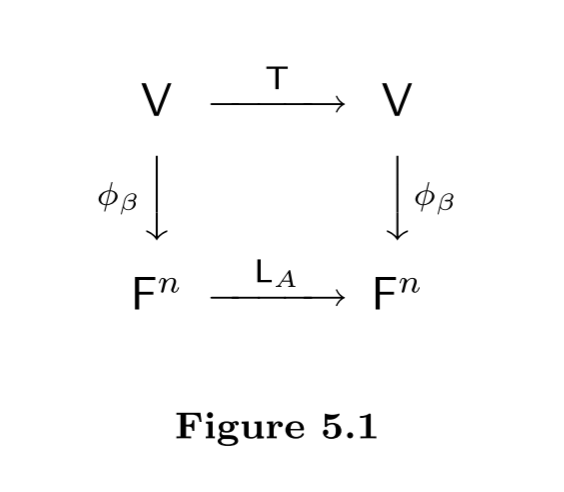
\includegraphics[width=8cm]{images/figure-5-1.png}

Recall that for \(v \in V\), (by \DEF{2.15}) \(\phi_{\beta}(v) = [v]_{\beta}\), the \emph{coordinate vector} of \(v\) \emph{relative to} \(\beta\).

We will show that \(v \in V\) is an eigenvector of \(\T\) corresponding to \(\lambda\) if and only if \(\phi_{\beta}(v)\) is an eigenvector of \(A\) corresponding to \(\lambda\).

Suppose that \(v\) is an eigenvector of \(\T\) corresponding to \(\lambda\).
Then \(v \ne \OV\) and \(\T(v) = \lambda v\) \MAROON{(1)}.
Hence
\begin{align*}
    A \phi_{\beta}(v) & = \LMTRAN_A \phi_{\beta} (v) & \text{by def of left multiplication} \\
        & = \phi_{\beta} \T(v) & \text{by Figure 5.1, the functions ``commute''} \\
        & = \phi_{\beta}(\T(v)) & \text{by def of function composition} \\
        & = \phi_{\beta}(\lambda v) & \text{by \MAROON{(1)}} \\
        & = \lambda \phi_{\beta}(v). & \text{\(\phi_{\beta}\) is linear, in particular}
\end{align*}
And since \(\phi_{\beta}\) is an isomorphism, \(\phi_{\beta}(v) \ne 0 \in F^n\);
hence \(\phi_{\beta}(v)\) is an eigenvector of \(A\) corresponding to \(\lambda\).

Now if \(\phi_{\beta}(v)\) is an eigenvector of \(A\) corresponding to \(\lambda\), then since the argument above is trivially ``reversible'', \(v\) is an eigenvector of \(\T\)
corresponding to \(\lambda\).
(See \EXEC{5.1.14}.)

An equivalent formulation of the result discussed in the preceding paragraph is that for an eigenvalue \(\lambda\) of \(A\) (and hence of \(\T\)),
a vector \(y \in F^n\) is an eigenvector of \(A\) corresponding to \(\lambda\) if and only if \(\phi_{\beta}^{-1}(y)\) is an eigenvector of \(\T\) corresponding to \(\lambda\).

Thus we have \emph{reduced} the problem of finding the eigenvectors \emph{of a linear operator} on a finite-dimensional vector space to the problem of finding the
eigenvectors \emph{of a matrix}.
The next example illustrates this procedure.
\end{remark}

\begin{note}
這邊只是在說,要找一個線性變換的\ eigenvector,可以找這個線性變換「的矩陣代表」的\ eigenvector,該\ vector 其實就是線性變換的某個\ eigenvector 的「座標向量」;
找到該座標向量後把它「轉回」(i.e. 用\ \(\phi_{\beta}^{-1}\) 轉)線性變換的向量即可。
\end{note}

\begin{example} \label{example 5.1.7}
Let \(\T(f(x)) = f(x) + (x + 1)f'(x)\) be the linear operator on \(\POLYRR\) defined in \EXAMPLE{5.1.5},
and let \(\beta\) be the standard ordered basis for \(\POLYRR\).
Recall that \(\T\) has eigenvalues \(1, 2\), and \(3\) and that
\[
    A = [\T]_{\beta} = \begin{pmatrix} 1 & 1 & 0 \\ 0 & 2 & 2 \\ 0 & 0 & 3 \end{pmatrix}.
\]
We consider each eigenvalue separately.

Let \(\lambda_{1}=1\), and define
\
\[
    B_{1}=A-\lambda_{1} I=\left(\begin{array}{lll}
        0 & 1 & 0 \\
        0 & 1 & 2 \\
        0 & 0 & 2
    \end{array}\right).
\]
Then
\[
    x=\left(\begin{array}{l} x_{1} \\ x_{2} \\ x_{3} \end{array}\right) \in \SET{R}^{3}
\]
is an eigenvector corresponding to \(\lambda_{1}=1\) if and only if \(x \ne 0\) and \(x \in \NULL \left( \LMTRAN_{B_{1}} \right)\);
that is, \(x\) is a nonzero solution to the system
\[
    \sysdelim..\systeme{
        x_{2}=0,
        x_{2}+2 x_{3}=0,
        2 x_{3}=0
    }.
\]
Notice that this system has three unknowns, \(x_1, x_2\), and \(x_3\), but one of these, \(x_1\), does not actually appear in the system.
Since the values of \(x_1\) do not affect the system, we assign \(x_1\) a parametric value, say \(x_1 = a\), and solve the system for \(x_2\) and \(x_3\).
Clearly, \(x_2 = x_3 = 0\), and so the eigenvectors \MAROON{of \(A\)} corresponding to \(\lambda_1 = 1\) are of the form
\[
    a \begin{pmatrix} 1 \\ 0 \\ 0 \end{pmatrix} = a e_1
\]
for \(a \ne 0\).
Consequently, the eigenvectors \MAROON{of \(\T\)} corresponding to \(\lambda_1 = 1\) are of the form
\[
    \phi_{\beta}^{-1}\left(a e_{1}\right)=a \phi_{\beta}^{-1}\left(e_{1}\right)=a \cdot 1=a \in \mathcal{P}_2(\SET{R}^2)
\]
for any \(a \ne 0\).
Hence the nonzero constant polynomials are the eigenvectors of \(\T\) corresponding to \(\lambda_1 = 1\).

Next let \(\lambda_2 = 2\), and define
\[
    B_{2}=A-\lambda_{2} I=\left(\begin{array}{lll}
        -1 & 1 & 0 \\
        0 & 0 & 2 \\
        0 & 0 & 1
    \end{array}\right).
\]
It is easily verified that
\[
    \NULL(\LMTRAN_{B_2}) = \left\{ a \begin{pmatrix} 1 \\ 1 \\ 0 \end{pmatrix} : a \in \SET{R} \right\}.
\]
and hence the eigenvectors of \(\T\) corresponding to \(\lambda_2 = 2\) are of the form
\[
    \phi_{\beta}^{-1} \left( a \begin{pmatrix} 1 \\ 1 \\ 0 \end{pmatrix} \right) = a \phi_{\beta}^{-1} (e_1 + e_2) = a (1 + x) = a + x
\]
for \(a \ne 0\).

Finally, consider \(\lambda_{3} = 3\) and
\[
    B_{3}=A-\lambda_{3} I=\left(\begin{array}{rrr}
        -2 & 1 & 0 \\
        0 & -1 & 2 \\
        0 & 0 & 0
    \end{array}\right)
\]
Since
\[
    \NULL\left(\LMTRAN_{B_{3}}\right) = \left\{ a\left(\begin{array}{l} 1 \\ 2 \\ 1 \end{array}\right): a \in \SET{R} \right\},
\]
the eigenvectors of \(\T\) corresponding to \(\lambda_{3}=3\) are of the form
\[
    \phi_{\beta}^{-1}\left(a\left(\begin{array}{l} 1 \\ 2 \\ 1 \end{array}\right)\right)
    = a \phi_{\beta}^{-1}\left(e_{1}+2 e_{2}+e_{3}\right)
    = a \left(1+2 x+x^{2}\right) = a + 2ax + ax^2
\]
for \(a \ne 0\).

For each eigenvalue, select the corresponding eigenvector with \(a = 1 \ne 0\) in the preceding descriptions to obtain \(\gamma = \{ 1, 1 + x, 1 + 2x + x^2 \}\), which is an ordered
basis for \(\POLYRR\) consisting of eigenvectors of \(\T\).
Thus \(\T\) is diagonalizable, and
\[
    [\T]_{\gamma} = \begin{pmatrix} 1 & 0 & 0 \\ 0 & 2 & 0 \\ 0 & 0 & 3 \end{pmatrix}.
\]
\end{example}

We close this section with a \textbf{geometric description} of how a linear operator \(\T\) acts on an eigenvector in the context of a vector space \(V\) over \(\SET{R}\).
(Also see this \href{https://www.youtube.com/watch?v=PFDu9oVAE-g&ab_channel=3Blue1Brown}{video}.)
Let \(v\) be an eigenvector of \(\T\) and \(\lambda\) be the corresponding eigenvalue.
We can think of \(W = \spann(\{ v \})\), the one-dimensional subspace of \(V\) spanned by \(v\), as a line in \(V\) that passes through \(\OV\) and \(v\).
For any \(w \in W, w = cv\) for some scalar \(c\),
and hence
\[
    \T(w) = \T(cv) = c\T(v) = c (\lambda v) = \lambda (c v) = \lambda w;
\]
so \(\T\) acts on the vectors in \(W\) by \textbf{multiplying} each such vector by \(\lambda\).

There are several possible ways for \(\T\) to act on the vectors in \(W\), depending on the value of \(\lambda\).
We consider several cases. (See Figure 5.2.)

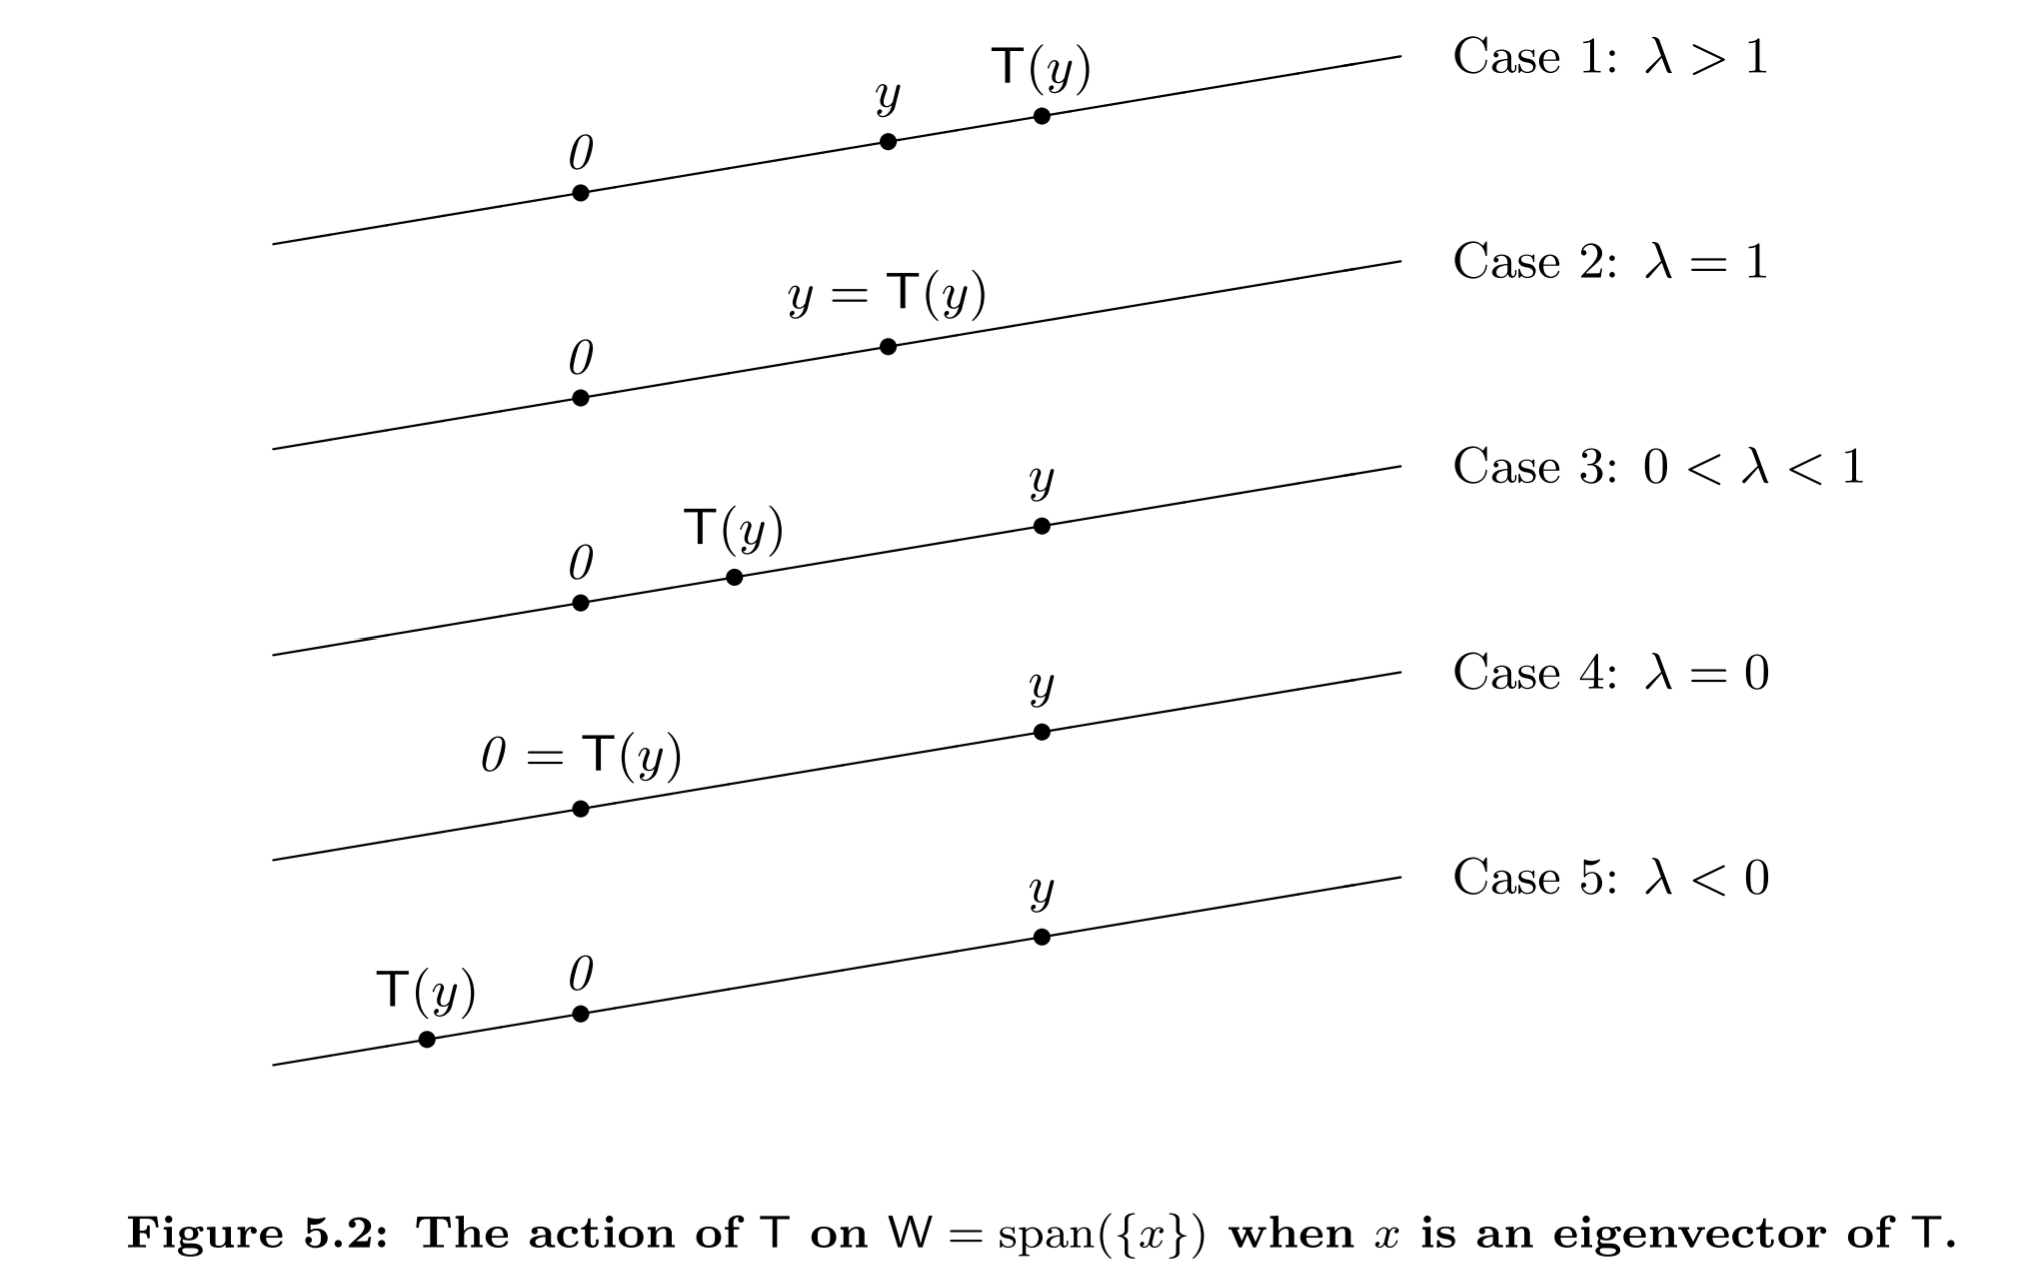
\includegraphics[width=17cm]{images/figure-5-2.png}

\begin{enumerate}
\item[CASE 1.] If \(\lambda > 1\), then \(\T\) moves vectors in \(W\) \emph{farther} from \(\OV\) by a factor of \(\lambda\).
\item[CASE 2.] If \(\lambda = 1\), then \(\T\) acts as the \emph{identity operator} on \(W\).
\item[CASE 3.] If \(\OF < \lambda < 1\), then \(\T\) moves vectors in \(W\) \emph{closer} to \(\OV\) by a factor of \(\lambda\).
\item[CASE 4.] If \(\lambda = \OF\), then \(\T\) acts as the \emph{zero transformation} on \(W\).
\item[CASE 5.] If \(\lambda < \OF\), then \(\T\) \emph{reverses the orientation} of \(W\); that is, \(\T\) moves vectors in \(W\) from one side of \(\OV\) to the other.
\end{enumerate}

To illustrate these ideas, we consider the linear operators in \EXAMPLE{2.1.3}, \EXAMPLE{2.1.4}, and \EXAMPLE{2.1.2}.

For the operator \(\T\) on \(\SET{R}^2\) defined by \(\T(a_1, a_2) = (a_1, -a_2)\), the \emph{reflection} about the \(x\)-axis, \(e_1\) and \(e_2\) are eigenvectors of \(\T\) with corresponding eigenvalues \(1\) and \(-1\), respectively.
Since \(e_1\) and \(e_2\) span the \(x\)-axis and the \(y\)-axis, respectively, \(\T\) \emph{acts as the identity} on the \(x\)-axis and \emph{reverses the orientation}
of the \(y\)-axis.

For the operator \(\T\) on \(\SET{R}^2\) defined by \(\T(a_1, a_2) = (a_1, 0)\), the \emph{projection} on the \(x\)-axis, \(e_1\) and \(e_2\) are eigenvectors of \(\T\) with corresponding eigenvalues \(1\) and \(0\), respectively.
Thus, \(\T\) acts as the identity on the \(x\)-axis and as the \emph{zero operator} on the \(y\)-axis.

Finally, we generalize \EXAMPLE{2.1.2} of this section by considering the operator that \emph{rotates} the plane through the angle, which is defined by
\[
    \T_{\theta}(a_1, a_2) = (a_1 \cos \theta - a_2 \sin \theta, a_1 \sin \theta + a_2 \cos \theta).
\]
Suppose that \(0 < \theta < \pi\).
Then for any nonzero vector \(v\), the vectors \(v\) and \(\T_{\theta}(v)\) are \textbf{not collinear}, and hence \(\T_{\theta}\) maps no one-dimensional subspace of \(\SET{R}^2\) into itself.
But this implies that \(\T_{\theta}\) \emph{has no eigenvectors} and therefore no eigenvalues.
To confirm this conclusion, let \(\beta\) be the standard ordered basis for \(\SET{R}^2\), and note that the \CPOLY{} of \(\T_{\theta}\) is
\[
    \det\left(\left[\T_{\theta}\right]_{\beta}-t I_{2}\right)
    = \det \begin{pmatrix}
        \cos \theta-t & -\sin \theta \\
        \sin \theta & \cos \theta-t
    \end{pmatrix}
    = t^{2} - (2 \cos \theta) t + 1
\]
which has no \textbf{real} zeros because, for \(0 < \theta < \pi\), the discriminant \(4 \cos^2 \theta - 4\) is negative.

\begin{remark} \label{remark 5.1.10}
However, the rotation operator in the previous discussion \emph{does have} eigenvalues when the field is \emph{complex number}, and \(\pm \iu\) are the eigenvalue of this transformation.
In addition, the ``geometric explanation'' in the discussion no longer applies, since it does not correctly describe the ``geometry'' of complex number.
\end{remark}

\exercisesection

\begin{exercise} \label{exercise 5.1.1}
Label the following statements as true or false.
\begin{enumerate}
\item  Every linear operator on an \(n\)-dimensional vector space has \(n\) distinct eigenvalues.
\item If a real matrix has one eigenvector, then it has an infinite number of eigenvectors.
\item There exists a square matrix with no eigenvectors.
\item Eigenvalues must be nonzero scalars.
\item Any two eigenvectors are \LID{}.
\item The sum of two eigenvalues of a linear operator \(\T\) is also an eigenvalue of \(\T\).
\item Linear operators on infinite-dimensional vector spaces never have eigenvalues.
\item An \(n \X n\) matrix \(A\) with entries from a field \(F\) is similar to a diagonal matrix if and only if there is a basis for \(F^n\) consisting of eigenvectors of \(A\).
\item Similar matrices always have the same eigenvalues.
\item Similar matrices always have the same eigen\RED{vectors}.
\item The sum of two eigenvectors of an operator \(\T\) is always an eigenvector of \(\T\).
\end{enumerate}
\end{exercise}

\begin{proof} \ 

\begin{enumerate}
\item False. Identity mapping on \(\SET{R}^{\RED{2}}\) has only \(\RED{1}\) eigenvalue \(\lambda = 1\).
\item True. If \(\T(v) = \lambda v\), then given any scalar \(c \ne 0\), \(\T(cv) = c \T(v) = c (\lambda v) = \lambda (c v)\).
\item True. Rotation on \(\SET{R}^2\) is an example.
\item False. Zero transformation has \(0\) as eigenvalue.
\item False. Part (b) is a counterexample.
\item False. Counterexample: \(1\) is an eigenvalue of the identity transformation, but \(1 + 1 = 2\) is not an eigenvalue of the identity transformation.
\item False. \EXAMPLE{5.1.3} is a counterexample.
\item True. This is directly implied by \CORO{5.1.1}.
\item True by \EXEC{5.1.13}: Having same \CPOLY{}s implies having same eigenvalues.
\item False. Counterexample:
    The matrices \(\left(\begin{array}{ll}1 & 1 \\ 0 & 2\end{array}\right)\) and \(\left(\begin{array}{ll}2 & 0 \\ 1 & 1\end{array}\right)\)  are similar since
    \[
        \left(\begin{array}{ll} 0 & 1 \\ 1 & 0 \end{array}\right)
        \left(\begin{array}{ll} 1 & 1 \\ 0 & 2 \end{array}\right)
        \left(\begin{array}{ll} 0 & 1 \\ 1 & 0 \end{array}\right)
        = \left(\begin{array}{ll} 2 & 0 \\ 1 & 1 \end{array}\right).
    \]
    But the eigenvector \((1,0)\) of the first matrix is not a eigenvector of the second matrix.

\item False. By part(b), if \(v\) is an eigenvector, then \(-1 \cdot v = -v\) is also an eigenvector, but \(v + -v = \OV\), which by definition is not an eigenvector.
\end{enumerate}
\end{proof}

\begin{exercise} \label{exercise 5.1.2}
For each of the following linear operators \(\T\) on a vector space \(V\), compute the determinant of \(\T\) and the \CPOLY{} of \(\T\).
\begin{enumerate}
\item \(V = \SET{R}^2, \T\begin{pmatrix}a \\ b\end{pmatrix}=\begin{pmatrix}2 a-b \\ 5 a+3 b\end{pmatrix}\)
\item \(V = \SET{R}^{3}, \T\begin{pmatrix}a \\ b \\ c\end{pmatrix}=\begin{pmatrix}a-3 b+2 c \\ -2 a+b+c \\ 4 a-c\end{pmatrix}\)
\item \(V = \mathcal{P}_{3}(\SET{R}), \T\left(a+b x+c x^{2}+d x^{3}\right)=(a-c)+(-a+b+d) x+(a+b-d) x^{2}-c x^{3}\)
\item \(V = M_{2 \X 2}(\SET{R}), \T(A) = 2 A^\top - A\)
\end{enumerate}
\end{exercise}

\begin{proof} \ 

\begin{enumerate}
\item Let \(\beta\) be standard ordered basis for \(\SET{R}^2\).
Then
\begin{align*}
    \det(\T) & = \det([\T]_{\beta}) & \text{by \DEF{5.4}} \\
             & = \det \begin{pmatrix} 2 & -1 \\ 5 & 3  \end{pmatrix} = 11.
\end{align*}
And the \CPOLY{} of \(\T\), by \DEF{5.4}, is
\begin{align*}
    \det([\T]_{\beta} - tI_2) & = \det \begin{pmatrix}
        2-t & -1 \\ 5 & 3-t
    \end{pmatrix} \\
        & = (2 - t)(3 - t) + 5 = t^2 - 5t + 11.
\end{align*}

\item Let \(\beta\) be standard ordered basis for \(\SET{R}^3\).
Then
\begin{align*}
    \det(\T) & = \det([\T]_{\beta}) & \text{by \DEF{5.4}} \\
             & = \det \begin{pmatrix} 1 & -3 & 2 \\ -2 & 1 & 1 \\ 4 & 0 & -1 \end{pmatrix} = -15.
\end{align*}
And the \CPOLY{} of \(\T\), by \DEF{5.4}, is
\begin{align*}
    \det([\T]_{beta} - tI_3) & = \begin{pmatrix} 1-t & -3 & 2 \\ -2 & 1-t & 1 \\ 4 & 0 & -1-t \end{pmatrix} \\
        & = -t^3 + t^2 + 15t - 15 & \text{by calculation}
\end{align*}
\item
Let \(\beta = \{ 1, x, x^2, x^3 \}\) be standard ordered basis for \(\POLYRRR\).
Then
\begin{align*}
    \T(1) & = 1 - x + x^2 + 0x^3, \\
    \T(x) & = 0 + x + x^2 + 0x^3, \\
    \T(x^2) & = -1 + 0x + 0x^2 - x^3, \\
    \T(x^3) & = 0 + 0x - x^2 + 0x^3,
\end{align*}
Hence by \DEF{5.4},
\[
    \det(\T) = \det([\T]_{\beta}) = \begin{pmatrix}
        1 & 0 & -1 & 0 \\
        -1 & 1 & 0 & 1 \\
        1 & 1 & 0 & -1 \\
        0 & 0 & -1 & 0
    \end{pmatrix} = -2.
\]
And the \CPOLY{} is
\[
    \det([\T]_{\beta} - tI_4) = \begin{pmatrix}
        1 - t & 0 & -1 & 0 \\
        -1 & 1 - t & 0 & 1 \\
        1 & 1 & 0 - t & -1 \\
        0 & 0 & -1 & 0 - t
    \end{pmatrix}
    = t^4 - 2t^3 + t^2 + t - 2.
\]

\item Let
\[
    \beta = \left\{
        \begin{pmatrix} 1 & 0 \\ 0 & 0 \end{pmatrix},
        \begin{pmatrix} 0 & 1 \\ 0 & 0 \end{pmatrix},
        \begin{pmatrix} 0 & 0 \\ 1 & 0 \end{pmatrix},
        \begin{pmatrix} 0 & 0 \\ 0 & 1 \end{pmatrix}
    \right\}
\]
be the standard ordered basis for \(M_{2 \X 2}(\SET{R})\).
Then
\begin{align*}
    \T \begin{pmatrix} 1 & 0 \\ 0 & 0 \end{pmatrix} & = \begin{pmatrix} 1 & 0 \\ 0 & 0 \end{pmatrix} \\
    \T \begin{pmatrix} 0 & 1 \\ 0 & 0 \end{pmatrix} & = \begin{pmatrix} 0 & -1 \\ 2 & 0 \end{pmatrix} \\
    \T \begin{pmatrix} 0 & 0 \\ 1 & 0 \end{pmatrix} & = \begin{pmatrix} 0 & 2 \\ -1 & 0 \end{pmatrix} \\
    \T \begin{pmatrix} 0 & 0 \\ 0 & 1 \end{pmatrix} & = \begin{pmatrix} 0 & 0 \\ 0 & 1 \end{pmatrix}
\end{align*}
Then clearly, by \DEF{5.4},
\[
    \det(\T) = \det([\T]_{\beta}) = \begin{pmatrix}
        1 & 0 & 0 & 0 \\
        0 & -1 & 2 & 0 \\
        0 & 2 & -1 & 0 \\
        0 & 0 & 0 & 1
    \end{pmatrix} = -3.
\]
And the \CPOLY{} is
\[
    \det([\T]_{\beta} - t I_4) = \begin{pmatrix}
        1-t & 0 & 0 & 0 \\
        0 & -1-t & 2 & 0 \\
        0 & 2 & -1-t & 0 \\
        0 & 0 & 0 & 1-t
    \end{pmatrix} = t^4 - 6t^2 + 8t - 3.
\]
\end{enumerate}
\end{proof}

\begin{exercise} \label{exercise 5.1.3}
For each of the following linear operators \(\T\) on a vector space \(V\) and an ordered basis \(\beta\), compute \([\T]_{\beta}\), and determine whether \(\beta\) is a basis
consisting of eigenvectors of \(\T\).

\begin{enumerate}
\item
\(
    V = \mathrm{R}^{2}, \T\begin{pmatrix}a \\ b\end{pmatrix}=\begin{pmatrix}10 a-6 b \\ 17 a-10 b\end{pmatrix} , \text{ and } \beta=\left\{\begin{pmatrix}1 \\ 2\end{pmatrix},\begin{pmatrix}2 \\ 3\end{pmatrix}\right\}\)

\item
\(
    V=\mathcal{P}_{1}(\SET{R}), \T(a+b x)=(6 a-6 b)+(12 a-11 b) x ,
    \text{ and } \beta=\{3+4 x, 2+3 x\}
\)

\item
\(
    V=\mathrm{R}^{3}, \T\begin{pmatrix}a \\ b \\ c\end{pmatrix}=\begin{pmatrix}3 a+2 b-2 c \\ -4 a-3 b+2 c \\ -c\end{pmatrix},
    \text{ and } \\
    \beta=\left\{
        \begin{pmatrix} 0 \\ 1 \\ 1 \end{pmatrix},
        \begin{pmatrix} 1 \\ -1 \\ 0 \end{pmatrix},
        \begin{pmatrix} 1 \\ 0 \\ 2 \end{pmatrix}
    \right\}
\)

\item
\(
    V=\mathcal{P}_{2}(\SET{R}), \T\left(a+b x+c x^{2}\right)=  (-4 a+2 b-2 c)-(7 a+3 b+7 c) x+(7 a+b+5 c) x^{2},
    \text{ and } \\
    \beta=\left\{ x-x^{2},-1+x^{2},-1-x+x^{2}\right\}
\)

\item
\(
    V=\mathcal{P}_{3}(\SET{R}), \\
    \T\left(a+b x+c x^{2}+d x^{3}\right) = -d+(-c+d) x+(a+b-2 c) x^{2}+(-b+c-2 d) x^{3}, \\
    \text{ and }
    \beta=\left\{1-x+x^{3}, 1+x^{2}, 1, x+x^{2}\right\}
\)

\item
\(
    V=\mathrm{M}_{2 \times 2}(\SET{R}), \T\begin{pmatrix}a & b \\ c & d\end{pmatrix}=\begin{pmatrix}-7 a-4 b+4 c-4 d & b \\ -8 a-4 b+5 c-4 d & d\end{pmatrix}, \\
    \text{ and }
    \beta=\left\{
        \begin{pmatrix} 1 & 0 \\ 1 & 0 \end{pmatrix},
        \begin{pmatrix} -1 & 2 \\ 0 & 0 \end{pmatrix},
        \begin{pmatrix} 1 & 0 \\ 2 & 0 \end{pmatrix},
        \begin{pmatrix} -1 & 0 \\ 0 & 2 \end{pmatrix}
    \right\}
\)
\end{enumerate}
\end{exercise}

\begin{proof}
I only calculate \([\T]_{\beta}\) when \(\beta\) is actually an eigenvector basis.

\begin{enumerate}
\item
\[
    \T \begin{pmatrix} 1 \\ 2 \end{pmatrix} = \begin{pmatrix}
        10 \cdot 1 - 6 \cdot 2 \\
        17 \cdot 1 - 10 \cdot 2
    \end{pmatrix}
    = \begin{pmatrix}
        -2 \\ -3
    \end{pmatrix} \ne \lambda \begin{pmatrix} 1 \\ 2 \end{pmatrix} \text{ for any } \lambda \in \SET{R}.
\]
Hence \(\beta\) is not an eigenvector basis for \(\T\).

\item
\[
    \T(3 + 4x) = (6 \cdot 3 - 6 \cdot 4) + (12 \cdot 3 - 11 \cdot 4)x = -6 + -8x = -2(3 + 4x),
\]
so \(3 + 4x\) is an eigenvector corresponding to \(-2\).
Similarly, \(\T(2 + 3x) = -3(2 + 3x)\), so \(2 + 3x\) is an eigenvector corresponding to \(-3\).
So \(\beta\) is an eigenvector basis, and \([\T]_{\beta} = \begin{pmatrix} -2 & 0 \\ 0 & -3 \end{pmatrix}\).

\item
\begin{align*}
    \T \begin{pmatrix} 0 \\ 1 \\ 1 \end{pmatrix} & = \begin{pmatrix} 0 \\ -1 \\ -1 \end{pmatrix} = -1 \begin{pmatrix} 0 \\ 1 \\ 1 \end{pmatrix} \\
    \T \begin{pmatrix} 1 \\ -1 \\ 0 \end{pmatrix} & = \begin{pmatrix} 1 \\ -1 \\ 0 \end{pmatrix} = 1 \begin{pmatrix} 1 \\ -1 \\ 0 \end{pmatrix} \\
    \T \begin{pmatrix} 1 \\ 0 \\ 2 \end{pmatrix} & = \begin{pmatrix} -1 \\ 0 \\ -2 \end{pmatrix} = -1 \begin{pmatrix} 1 \\ 0 \\ 2 \end{pmatrix}
\end{align*}
So \(\beta\) is an eigenvector basis with eigenvalues \(-1, 1\), and \([\T]_{\beta} = \begin{pmatrix} -1 & 0 & 0 \\ 0 & 1 & 0 \\ 0 & 0 & -1 \end{pmatrix}\).

\item
\begin{align*}
    \T(x - x^2) & = \T(0 + x - x^2) \\
        & =(0 + 2 + 2) - (0 - 3 + 7)x + (0 + 1 - 5)x^2 \\
        & = 4 + 4x - 4x^2
        \ne \lambda (x - x^2) \text{ for any \(\lambda \in \SET{R}\)},
\end{align*}
Hence \(\beta\) is not an eigenvector basis for \(\T\).

\item Skip, this is similar to part(d).

\item
\begin{align*}
    \T \begin{pmatrix} 1 & 0 \\ 1 & 0 \end{pmatrix}
        & = \begin{pmatrix} -7 - 0 + 4 - 0 & 0 \\ -8 - 0 + 5 - 0 & 0 \end{pmatrix}
          = \begin{pmatrix} -3 & 0 \\ -3 & 0 \end{pmatrix} = -3 \begin{pmatrix} 1 & 0 \\ 1 & 0 \end{pmatrix} \\
    \T \begin{pmatrix} -1 & 2 \\ 0 & 0 \end{pmatrix}
        & = \begin{pmatrix} 7 - 8 + 0 - 0 & 2 \\ 8 - 8 + 0 - 0 & 0 \end{pmatrix}
          = \begin{pmatrix} -1 & 2 \\ 0 & 0 \end{pmatrix} = 1 \begin{pmatrix} -1 & 2 \\ 0 & 0 \end{pmatrix} \\
    \T \begin{pmatrix} 1 & 0 \\ 2 & 0 \end{pmatrix}
        & = \begin{pmatrix} -7 - 0 + 8 - 0 & 0 \\ -8 - 0 + 10 - 0 & 0 \end{pmatrix}
          = \begin{pmatrix} 1 & 0 \\ 2 & 0 \end{pmatrix} = 1 \begin{pmatrix} 1 & 0 \\ 2 & 0 \end{pmatrix} \\
    \T \begin{pmatrix} -1 & 0 \\ 0 & 2 \end{pmatrix}
        & = \begin{pmatrix} 7 - 0 + 0 - 8 & 0 \\ 8 - 0 + 0 - 8 & 2 \end{pmatrix}
          = \begin{pmatrix} -1 & 0 \\ 0 & 2 \end{pmatrix} = 1 \begin{pmatrix} -1 & 0 \\ 0 & 2 \end{pmatrix},
\end{align*}
Hence \(\beta\) is an eigenvector basis for \(\T\), with eigenvalues \(-3, 1\),
and \([\T]_{\beta} = \begin{pmatrix} -3 & 0 & 0 & 0 \\ 0 & 1 & 0 & 0 \\ 0 & 0 & 1 & 0 \\ 0 & 0 & 0 & 1 \end{pmatrix}\).
\end{enumerate}
\end{proof}

\begin{exercise} \label{exercise 5.1.4}
For each of the following matrices \(A \in M_{n \X n}(F)\),
\begin{enumerate}
\item[(i)] Determine all the eigenvalues of \(A\).
\item[(ii)] For each eigenvalue \(\lambda\) of A, find the set of eigenvectors corresponding to \(\lambda\).
\item[(iii)] If possible, find a basis for \(F^n\) consisting of eigenvectors of \(A\).
\item[(iv)] If successful in finding such a basis, determine an invertible matrix \(Q\) and a diagonal matrix \(D\) such that \(Q^{-1} A Q = D\).
\end{enumerate}

\begin{enumerate}
\item \(
    A = \begin{pmatrix} 1 & 2 \\ 3 & 2 \end{pmatrix} \text{ for } F = \SET{R}. \)
\item \(
    A = \begin{pmatrix} 0 & -2 & -3 \\ -1 & 1 & -1 \\ 2 & 2 & 5 \end{pmatrix} \text{ for } F = \SET{R}. \)
\item \(
    A = \begin{pmatrix} \iu & 1 \\ 2 & -\iu \end{pmatrix} \text{ for } F = \SET{C}. \)
\item \(
    A = \begin{pmatrix} 2 & 0 & -1 \\ 4 & 1 & -4 \\ 2 & 0 & -1 \end{pmatrix} \text{ for } F = \SET{R}. \)
\end{enumerate}
\end{exercise}

\begin{proof} \ 

\begin{enumerate}
\item The \CPOLY{} of \(A\) is
\begin{align*}
    \det(A - tI_2) & = \det \begin{pmatrix}
        1-t & 2 \\ 3 & 2-t
    \end{pmatrix} \\
        & = (1 - t)(2 - t) - 6 = t^2 - 3t - 4 = (t - 4)(t + 1).
\end{align*}
So the eigenvalues are \(\lambda_1 = 4, \lambda_2 = -1\).
Now we first find the eigenvectors corresponding to \(\lambda_1\).
So let
\[
    B_1 = A - \lambda_1 I_2 = \begin{pmatrix}
        -3 & 2 \\ 3 & 2
    \end{pmatrix}.
\]
Clearly \(\NULL(B_1) = \left\{ t \begin{pmatrix} 1 \\ \frac{3}{2} \end{pmatrix} : t \in \SET{R} \right\}\).
So in particular let \(t = 2\), then \(v_1 = \begin{pmatrix} 2 \\ 3 \end{pmatrix}\) is an eigenvector corresponding to \(\lambda_1\).

Similarly, for \(\lambda_2\), let
\[
    B_2 = A - \lambda_2 I_2 = \begin{pmatrix}
        2 & 2 \\ 3 & 3
    \end{pmatrix}.
\]
Clearly \(\NULL(B_2) = \left\{ t \begin{pmatrix} 1 \\ -1 \end{pmatrix} : t \in \SET{R} \right\}\).
So in particular let \(t = 1\), then \(v_2 = \begin{pmatrix} 1 \\ -1 \end{pmatrix}\) is an eigenvector corresponding to \(\lambda_2\).
And by \CORO{5.1.1},
\[
    Q = \begin{pmatrix} v_1 & v_2 \end{pmatrix}
      = \begin{pmatrix}
            2 & 1 \\
            3 & -1
        \end{pmatrix}
\]
is the invertible matrix such that \(Q^{-1} A Q = D = \begin{pmatrix}
    \lambda_1 & 0 \\ 0 & \lambda_2 \end{pmatrix}\).

\item Skip, similar to part(a).

\item The \CPOLY{} of \(A\) is
\begin{align*}
    \det(A - tI_2) & = \det \begin{pmatrix}
        \iu - t & 1 \\ 2 & -\iu - t
    \end{pmatrix} \\
        & = (\iu - t)(-\iu - t) - 2 = -\iu^2 + t\iu - t\iu + t^2 - 2 = t^2 - 1 = (t - 1)(t + 1)
\end{align*}
So the eigenvalues are \(\lambda_1 = 1, \lambda_2 = -1\).
Now we first the eigenvectors corresponding to \(\lambda_1\).
So let
\[
    B_1 = A - \lambda_1 I_2 = \begin{pmatrix}
        \iu - 1 & 1 \\ 2 & -\iu - 1
    \end{pmatrix}.
\]
Applying an elementary operation that adds row \(1\) \textbf{times \RED{\(\iu + 1\)}} to row \(2\), we have
\[
    B' = \lambda_1 I_2 = \begin{pmatrix}
        \iu - 1 & 1 \\ 0 & 0
    \end{pmatrix}.
\]
That implies we have the (equivalent) system
\[
    (\iu - 1) x_1 + x_2 = 0.
\]
Let \(x_1\) be the parametric variable \(t\), then \(x_2 = -(\iu - 1)t\).
So
\[
    \NULL(B_1) = \left\{ t \begin{pmatrix} 1 \\ -(\iu - 1) \end{pmatrix} : t \in \SET{C} \right\}.
\]
So in particular let \(t = 1\), then \(v_1 = \begin{pmatrix} 1 \\ -\iu + 1 \end{pmatrix}\) is an eigenvector corresponding to \(\lambda_1\).

Similarly, for \(\lambda_2\), let
\[
    B_2 = A - \lambda_2 I_2 = \begin{pmatrix}
        \iu + 1 & 1 \\ 2 & -\iu + 1
    \end{pmatrix}.
\]
Again the equivalent system, by adding row \(1\) \textbf{times \(\iu - 1\)} to row \(2\), is
\[
    B' = \lambda_1 I_2 = \begin{pmatrix}
        \iu + 1 & 1 \\ 0 & 0
    \end{pmatrix}.
\]
That implies we have the (equivalent) system
\[
    (\iu + 1) x_1 + x_2 = 0.
\]
Let \(x_1\) be the parametric variable \(t\), then \(x_2 = -(\iu + 1)t\).
So
\[
    \NULL(B_2) = \left\{ t \begin{pmatrix} 1 \\ -(\iu + 1) \end{pmatrix} : t \in \SET{C} \right\}.
\]
So in particular let \(t = 1\), then \(v_2 = \begin{pmatrix} 1 \\ -\iu - 1 \end{pmatrix}\) is an eigenvector corresponding to \(\lambda_2\).

And by \CORO{5.1.1},
\[
    Q = \begin{pmatrix} v_1 & v_2 \end{pmatrix}
      = \begin{pmatrix}
            1        & 1 \\
            -\iu + 1 & -\iu - 1
        \end{pmatrix}
\]
is the invertible matrix such that \(Q^{-1} A Q = D = \begin{pmatrix}
    \lambda_1 & 0 \\ 0 & \lambda_2 \end{pmatrix}\).
    
\item The \CPOLY{} of \(A\) is
\begin{align*}
    \det(A - tI_3) & = \det \begin{pmatrix}
        2 - t & 0 & -1 \\ 4 & 1-t & -4 \\ 2 & 0 & -1 - t
    \end{pmatrix} \\
        & = (1 - t) \cdot [(2 - t)(-1 - t) + 2] & \text{by expanding second column} \\
        & = (1 - t) (t^2 - t + 0) = (1 - t)(t)(t - 1) \\
        & = -t(1 - t)^2
\end{align*}
So the eigenvalues are \(\lambda_1 = 0, \lambda_2 = 1\).
Now we first find the eigenvectors corresponding to \(\lambda_1\).
So let
\[
    B_1 = A - \lambda_1 I_3 = \begin{pmatrix}
        2 & 0 & -1 \\ 4 & 1 & -4 \\ 2 & 0 & -1
    \end{pmatrix}.
\]
By solving the system, \(\NULL(B_1) = \left\{ t \begin{pmatrix} \frac1{2} \\ 2 \\ 1 \end{pmatrix} : t \in \SET{R} \right\}\).
So in particular let \(t = 2\), then \(v_1 = \begin{pmatrix} 1 \\ 4 \\2 \end{pmatrix}\) is an eigenvector corresponding to \(\lambda_1\).

Similarly, for \(\lambda_2\), let
\[
    B_2 = A - \lambda_2 I_3 = \begin{pmatrix}
        1 & 0 & -1 \\ 4 & 0 & -4 \\ 2 & 0 & -2
    \end{pmatrix}.
\]
By solving the system \(\NULL(B_2) = \left\{ t_1 \begin{pmatrix} 1 \\ 0 \\ 1 \end{pmatrix} + t_2 \begin{pmatrix} 0 \\ 1 \\ 0 \end{pmatrix} : t_1, t_2 \in \SET{R} \right\}\).

Note that we have \emph{eigenspace} of dimension \(2\) for \(\lambda_2\) (see \DEF{5.7}), so we need to select two \LID{} eigenvectors from the space.
So in particular let \(t_1 = 1, t_2 = 0\), then \(v_2 = 1 \begin{pmatrix} 1 \\ 0 \\ 1 \end{pmatrix} + 0 \begin{pmatrix} 0 \\ 1 \\ 0 \end{pmatrix} = \begin{pmatrix} 1 \\ 0 \\ 1 \end{pmatrix}\) is an eigenvector corresponding to \(\lambda_2\).
And let \(t_1 = 0, t_2 = 1\), then \(v_3 = 0 \begin{pmatrix} 1 \\ 0 \\ 1 \end{pmatrix} + 1 \begin{pmatrix} 0 \\ 1 \\ 0 \end{pmatrix} = \begin{pmatrix} 0 \\ 1 \\ 0 \end{pmatrix}\) is \emph{another} eigenvector corresponding to \(\lambda_2\).
And by \CORO{5.1.1},
\[
    Q = \begin{pmatrix} v_1 & v_2 & v_3 \end{pmatrix}
      = \begin{pmatrix}
            1 & 1 & 0 \\
            4 & 0 & 1 \\
            2 & 1 & 0
        \end{pmatrix}
\]
is the invertible matrix such that \(Q^{-1} A Q = D = \begin{pmatrix}
    \lambda_1 & 0 & 0 \\ 0 & \lambda_2 & 0 \\ 0 & 0 & \lambda_3 \end{pmatrix}\).
\end{enumerate}
\end{proof}

\begin{exercise} \label{exercise 5.1.5}
For each linear operator \(\T\) on \(V\), find the eigenvalues of \(\T\) and an ordered basis \(\beta\) for \(V\) such that \([\T]_{\beta}\) is a diagonal matrix.
\begin{enumerate}
\item \(V = \SET{R}^2\) and \(\T(a, b) = (-2a + 3b, -10a + 9b)\)
\item \(V = \SET{R}^3\) and \(\T(a, b, c) = (7a - 4b + 10c, 4a - 3b + 8c, -2a + b - 2c)\)
\item \(V = \SET{R}^3\) and \(\T(a, b, c) = (-4a + 3b - 6c, 6a - 7b + 12c, 6a - 6b + 11c)\)
\item \(V = \mathcal{P}_1(\SET{R})\) and \(\T(ax + b) = (-6a + 2b)x + (-6a + b)\)
\item \(V = \POLYRR\) and \(\T(f(x)) = xf'(x) + f(2)x + f(3)\)
\item \(V = \POLYRRR\) and \(\T(f(x)) = f(x) + f(2)x\)
\item \(V = \POLYRRR\) and \(\T(f(x)) = xf'(x) + f''(x) - f(2)\)
\item \(V = M_{2 \X 2}(\SET{R})\) and \(\T \begin{pmatrix} a & b \\ c & d \end{pmatrix} = \begin{pmatrix} d & b \\ c & a \end{pmatrix}\)
\item \(V = M_{2 \X 2}(\SET{R})\) and \(\T \begin{pmatrix} a & b \\ c & d \end{pmatrix} = \begin{pmatrix} c & d \\ a & b \end{pmatrix}\)
\item \(V = M_{2 \X 2}(\SET{R})\) and \(\T(A) = A^\top + 2 \cdot \TRACE(A) \cdot I_2\).
\end{enumerate}
\end{exercise}

\begin{proof}
Just pick some items.

\begin{enumerate}
\item[(e)] Let \(\beta'\) be the standard ordered basis for \(\POLYRR\).
Then
\begin{align*}
    \T(1) & = x \cdot 0 + 1 \cdot x + 1 = 1 + x \\
    \T(x) & = x \cdot 1 + 2 \cdot x + 3 = 3 + 3x \\
    \T(x^2) & = x \cdot 2x + 4x + 9 = 9 + 4x + 2x^2 \\
    \implies & [\T]_{\beta'} = \begin{pmatrix}
        1 & 3 & 9 \\
        1 & 3 & 4 \\
        0 & 0 & 2
    \end{pmatrix}
\end{align*}
So the \CPOLY{} is
\begin{align*}
    \det([\T]_{\beta'} - tI_3) & = \begin{pmatrix}
        1-t & 3   & 9 \\
        1   & 3-t & 4 \\
        0   & 0   & 2-t
    \end{pmatrix} \\
    & = (2 - t)\left[ (1 - t)(3 - t) - 3 \right] & \text{by expanding last row} \\
    & = (2 - t)\left[ 3 - 3t - t + t^2 -3 \right] \\
    & = (2 - t)(-4t + t^2) \\
    & = (2 - t)(t)(t - 4)
\end{align*}
So the eigenvalues are \(\lambda_1 = 0, \lambda_2 = 2, \lambda_3 = 4\).
And by calculation, (or by WolframAlpha,) \(v_1 = (-3, 1, 0)\) is an eigenvector of \([\T]_{\beta'}\) with corresponding eigenvalue \(\lambda_1\),
\(v_2 = (-3, -13, 4)\) is an eigenvector of \([\T]_{\beta'}\) with corresponding eigenvalue \(\lambda_2\),
\(v_3 = (1, 1, 0)\) is an eigenvector of \([\T]_{\beta'}\) with corresponding eigenvalue \(\lambda_3\).

And by applying \(\phi_{\beta'}^{-1}\),
\(\phi_{\beta'}^{-1}(v_1) = -3 + x\) is an eigenvector of \(\T\) with corresponding eigenvalue  \(\lambda_1\),
\(\phi_{\beta'}^{-1}(v_2) = -3 -13x + 4x^2\) is an eigenvector of \(\T\) with corresponding eigenvalue \(\lambda_2\),
and \(\phi_{\beta'}^{-1}(v_3) = 1 + x\) is an eigenvector of \(\T\) with corresponding eigenvalue \(\lambda_3\),
And by \THM{5.1}, \(\beta = \{ -3 + x, -3 - 13x + 4x^2, 1 + x \}\) is a eigenvector basis for \(\POLYRR\) such that \([\T]_{\beta}\) is a diagonal matrix.

\item[(h)] Let \(\beta'\) be the standard ordered basis for \(M_{2 \X 2}(\SET{R})\).
Then
\begin{align*}
    \T \begin{pmatrix} 1 & 0 \\ 0 & 0 \end{pmatrix} & = \begin{pmatrix} 0 & 0 \\ 0 & 1 \end{pmatrix} \\
    \T \begin{pmatrix} 0 & 1 \\ 0 & 0 \end{pmatrix} & = \begin{pmatrix} 0 & 1 \\ 0 & 0 \end{pmatrix} \\
    \T \begin{pmatrix} 0 & 0 \\ 1 & 0 \end{pmatrix} & = \begin{pmatrix} 0 & 0 \\ 1 & 0 \end{pmatrix} \\
    \T \begin{pmatrix} 0 & 0 \\ 0 & 1 \end{pmatrix} & = \begin{pmatrix} 1 & 0 \\ 0 & 0 \end{pmatrix}
\end{align*}
So
\[
    [\T]_{\beta'} = \begin{pmatrix}
        0 & 0 & 0 & 1 \\
        0 & 1 & 0 & 0 \\
        0 & 0 & 1 & 0 \\
        1 & 0 & 0 & 0
    \end{pmatrix}
\]
And the \CPOLY{} is
\begin{align*}
    \det([\T]_{\beta'} - t I_4)
    & = \det \begin{pmatrix}
        -t & 0 & 0 & 1 \\
        0 & 1-t & 0 & 0 \\
        0 & 0 & 1-t & 0 \\
        1 & 0 & 0 & 0-t
    \end{pmatrix} \\
    & = (1+t)^2(1-t)^2 & \text{by calculation}
\end{align*}
So the eigenvalues are \(\lambda_1 = 1, \lambda_2 = -1\).
For \(\lambda_1 = 1\), let
\[
    B_1 = [\T]_{\beta'} - \lambda_1 I_4
    = \det \begin{pmatrix}
        -1 & 0 & 0 & 1 \\
        0 & 0 & 0 & 0 \\
        0 & 0 & 0 & 0 \\
        1 & 0 & 0 & 1
    \end{pmatrix}; \text{ the equivalent matrix is }
    \begin{pmatrix}
        1 & 0 & 0 & -1 \\
        0 & 0 & 0 & 0 \\
        0 & 0 & 0 & 0 \\
        0 & 0 & 0 & 0
    \end{pmatrix}
\]
which has the null space
\[
    \left\{ t_1 \begin{pmatrix} 1 \\ 0 \\ 0 \\ 1 \end{pmatrix} + t_2 \begin{pmatrix} 0 \\ 1 \\ 0 \\ 0 \end{pmatrix} + t_3 \begin{pmatrix} 0 \\ 0 \\ 1 \\ 0 \end{pmatrix} : t_1, t_2, t_3 \in \SET{R} \right\}
\]
Again this implies the eigenspace of \(\lambda_1\) has dimension \(3\), so we need to pick \(3\) \LID{} vectors in the space.

So if we let \(t_1 = 1, t_2 = 0, t_3 = 0\), we get eigenvector \(v_1 = \begin{pmatrix} 1 & 0 & 0 & 1 \end{pmatrix}^\top\) of \([\T]_{\beta'}\) with corresponding eigenvalue \(\lambda_1\);
if we let \(t_1 = 0, t_2 = 1, t_3 = 0\), we get eigenvector \(v_2 = \begin{pmatrix} 0 & 1 & 0 & 0 \end{pmatrix}^\top\) of \([\T]_{\beta'}\) with corresponding eigenvalue \(\lambda_1\);
if we let \(t_1 = 0, t_2 = 0, t_3 = 1\), we get eigenvector \(v_3 = \begin{pmatrix} 0 & 0 & 1 & 0 \end{pmatrix}^\top\) of \([\T]_{\beta'}\) with corresponding eigenvalue \(\lambda_1\);

For \(\lambda_2 = -1\), let
\[
    B_1 = [\T]_{\beta'} - \lambda_2 I_4
    = \det \begin{pmatrix}
        1 & 0 & 0 & 1 \\
        0 & 2 & 0 & 0 \\
        0 & 0 & 2 & 0 \\
        1 & 0 & 0 & 1
    \end{pmatrix}; \text{ the equivalent matrix is }
    \begin{pmatrix}
        1 & 0 & 0 & 1 \\
        0 & 1 & 0 & 0 \\
        0 & 0 & 1 & 0 \\
        0 & 0 & 0 & 0
    \end{pmatrix}
\]
which has the null space
\[
    \left\{ t \begin{pmatrix} -1 \\ 0 \\ 0 \\ 1 \end{pmatrix} : t \in \SET{R} \right\}
\]
So in particular let \(t = 1\), then \(v_4 = \begin{pmatrix} -1 & 0 & 0 & 1 \end{pmatrix}^\top\) is an eigenvector of \([\T]_{\beta'}\) with corresponding eigenvalue \(\lambda_2\).

And by applying \(\phi_{\beta'}^{-1}\),
\begin{center}
    \(\phi_{\beta'}^{-1}(v_1) = \begin{pmatrix} 1 & 0 \\ 0 & 1 \end{pmatrix}\) is an eigenvector of \(\T\) with corresponding eigenvalue \(\lambda_1\), \\
    \(\phi_{\beta'}^{-1}(v_2) = \begin{pmatrix} 0 & 1 \\ 0 & 0 \end{pmatrix}\) is an eigenvector of \(\T\) with corresponding eigenvalue \(\lambda_1\), \\
    \(\phi_{\beta'}^{-1}(v_3) = \begin{pmatrix} 0 & 0 \\ 1 & 0 \end{pmatrix}\) is an eigenvector of \(\T\) with corresponding eigenvalue \(\lambda_1\), \\
    \(\phi_{\beta'}^{-1}(v_4) = \begin{pmatrix} -1 & 0 \\ 0 & 1 \end{pmatrix}\) is an eigenvector of \(\T\) with corresponding eigenvalue \(\lambda_2\).
\end{center}
And by \THM{5.1},
\[
    \beta = \left\{
        \begin{pmatrix} 1 & 0 \\ 0 & 1 \end{pmatrix},
        \begin{pmatrix} 0 & 1 \\ 0 & 0 \end{pmatrix},
        \begin{pmatrix} 0 & 0 \\ 1 & 0 \end{pmatrix},
        \begin{pmatrix} -1 & 0 \\ 0 & 1 \end{pmatrix}
    \right\}
\]
is an eigenvector basis for \(M_{2 \X 2}(\SET{R})\) such that \([\T]_{\beta}\) is a diagonal matrix.

\item[(i)]
Let \(\beta\) be the standard ordered basis for \(M_{2 \X 2}(\SET{R})\).
Then
\begin{align*}
    \T \begin{pmatrix} 1 & 0 \\ 0 & 0 \end{pmatrix} & = \begin{pmatrix} 0 & 0 \\ 1 & 0 \end{pmatrix} \\
    \T \begin{pmatrix} 0 & 1 \\ 0 & 0 \end{pmatrix} & = \begin{pmatrix} 0 & 0 \\ 0 & 1 \end{pmatrix} \\
    \T \begin{pmatrix} 0 & 0 \\ 1 & 0 \end{pmatrix} & = \begin{pmatrix} 1 & 0 \\ 0 & 0 \end{pmatrix} \\
    \T \begin{pmatrix} 0 & 0 \\ 0 & 1 \end{pmatrix} & = \begin{pmatrix} 0 & 1 \\ 0 & 0 \end{pmatrix}
\end{align*}
So
\[
    [\T]_{\beta'} = \begin{pmatrix}
        0 & 0 & 1 & 0 \\
        0 & 0 & 0 & 1 \\
        1 & 0 & 0 & 0 \\
        0 & 1 & 0 & 0
    \end{pmatrix}
\]
And the \CPOLY{} is
\begin{align*}
    \det([\T]_{\beta'} - t I_4)
    & = \det \begin{pmatrix}
        -t & 0 & 1 & 0 \\
        0 & -t & 0 & 1 \\
        1 & 0 & -t & 0 \\
        0 & 1 & 0 & -t
    \end{pmatrix} \\
    & = (t - 1)^2(t + 1)^2 & \text{by calculation}
\end{align*}
So \(\lambda_1 = 1, \lambda_2\) are the eigenvectors of \([\T]_{\beta'}\).

By the similar process in the previous item,
for \(\lambda_1\), some corresponding two \LID{} eigenvectors are \(v_1 = (0, 1, 0, 1), v_2 = (1, 0, 1, 0)\);
for \(\lambda_2\), some corresponding two \LID{} eigenvectors are \(v_3 = (-1, 0, 1, 0), v_4 = (0, -1, 0, 1)\);
And
\[
    \beta = \{ \phi_{\beta'}^{-1}(v_1), \phi_{\beta'}^{-1}(v_2), \phi_{\beta'}^{-1}(v_3), \phi_{\beta'}^{-1}(v_4) \}
    = \left\{
        \begin{pmatrix} 0 & 1 \\ 0 & 1 \end{pmatrix},
        \begin{pmatrix} 1 & 0 \\ 1 & 0 \end{pmatrix},
        \begin{pmatrix} -1 & 0 \\ 1 & 0 \end{pmatrix},
        \begin{pmatrix} 0 & -1 \\ 0 & 1 \end{pmatrix}
    \right\}
\]
is an eigenvector basis for \(M_{2 \X 2}(\SET{R})\) such that \([\T]_{\beta}\) is a diagonal matrix.

\item[(j)]
Similarly as the previous item,
\begin{align*}
    \T \begin{pmatrix} 1 & 0 \\ 0 & 0 \end{pmatrix}
        & = \begin{pmatrix} 1 & 0 \\ 0 & 0 \end{pmatrix} + 2 \cdot 1 \cdot I_2
        = \begin{pmatrix} 3 & 0 \\ 0 & 1 \end{pmatrix} \\
    \T \begin{pmatrix} 0 & 1 \\ 0 & 0 \end{pmatrix}
        & = \begin{pmatrix} 0 & 0 \\ 1 & 0 \end{pmatrix} + 2 \cdot 0 \cdot I_2
        = \begin{pmatrix} 0 & 0 \\ 1 & 0 \end{pmatrix} \\
    \T \begin{pmatrix} 0 & 0 \\ 1 & 0 \end{pmatrix}
        & = \begin{pmatrix} 0 & 1 \\ 0 & 0 \end{pmatrix} + 2 \cdot 0 \cdot I_2
        = \begin{pmatrix} 0 & 1 \\ 0 & 0 \end{pmatrix} \\
    \T \begin{pmatrix} 0 & 0 \\ 0 & 1 \end{pmatrix}
        & = \begin{pmatrix} 0 & 0 \\ 0 & 1 \end{pmatrix} + 2 \cdot 1 \cdot I_2
        = \begin{pmatrix} 1 & 0 \\ 0 & 3 \end{pmatrix}
\end{align*}
So
\[
    [\T]_{\beta'} = \begin{pmatrix}
        3 & 0 & 0 & 1 \\
        0 & 0 & 1 & 0 \\
        0 & 1 & 0 & 0 \\
        1 & 0 & 0 & 3
    \end{pmatrix}
\]
And the \CPOLY{} is
\begin{align*}
    \det([\T]_{\beta'} - t I_4)
    & = \det \begin{pmatrix}
        3-t & 0   & 0   & 1 \\
        0   & 0-t & 1   & 0 \\
        0   & 1   & 0-t & 0 \\
        1   & 0   & 0 & 3 -t
    \end{pmatrix} \\
    & = (t - 4)(t - 2)(t - 1)(t + 1) & \text{by calculation}
\end{align*}
So \(\lambda_1 = -1, \lambda_2 = 1, \lambda_3 = 2, \lambda_4 = 4\) are the eigenvectors of \([\T]_{\beta'}\).

By the similar process in the previous item,
for \(\lambda_1\), a corresponding eigenvector is \(v_1 = (0, -1, 1, 0)\);
for \(\lambda_2\), a corresponding eigenvector is \(v_2 = (0, 1, 1, 0)\);
for \(\lambda_3\), a corresponding eigenvector is \(v_3 = (-1, 0, 0, 1)\);
for \(\lambda_4\), a corresponding eigenvector is \(v_4 = (1, 0, 0, 1)\);
And
\[
    \beta = \{ \phi_{\beta'}^{-1}(v_1), \phi_{\beta'}^{-1}(v_2), \phi_{\beta'}^{-1}(v_3), \phi_{\beta'}^{-1}(v_4) \}
    = \left\{
        \begin{pmatrix} 0 & -1 \\ 1 & 0 \end{pmatrix},
        \begin{pmatrix} 0 & 1 \\ 1 & 0 \end{pmatrix},
        \begin{pmatrix} -1 & 0 \\ 0 & 1 \end{pmatrix},
        \begin{pmatrix} 1 & 0 \\ 0 & 1 \end{pmatrix}
    \right\}
\]
is an eigenvector basis for \(M_{2 \X 2}(\SET{R})\) such that \([\T]_{\beta}\) is a diagonal matrix.
\end{enumerate}
\end{proof}

\begin{exercise} \label{exercise 5.1.6}
Prove \THM{5.4}.
\end{exercise}

\begin{proof}
See \THM{5.4}.
\end{proof}

\begin{exercise} \label{exercise 5.1.7}
Let \(\T\) be a linear operator on a finite-dimensional vector space \(V\), and let \(\beta\) be an ordered basis for \(V\).
Prove that \(\lambda\) is an eigenvalue of \(\T\) if
and only if \(\lambda\) is an eigenvalue of \([\T]_{\beta}\).
\end{exercise}

\begin{proof}
This is described in \RMK{5.1.7} (Precisely, that remark uses \EXEC{5.1.13}.)
\end{proof}

\begin{exercise} \label{exercise 5.1.8}
Let \(\T\) be a linear operator on a finite-dimensional vector space \(V\).
Refer to the definition of the determinant of \(\T\) (\DEF{5.4}) to prove the following results.
\begin{enumerate}
\item Prove that this definition is independent of the choice of an ordered basis for \(V\).
That is, prove that if \(\beta\) and \(\gamma\) are two ordered bases for \(V\), then \(\det([\T]_{\beta}) = \det([\T]_{\gamma})\).
\item Prove that \(\T\) is invertible if and only if \(\det(\T) \ne 0\).
\item Prove that if \(\T\) is invertible, then \(\det(\T^{-1}) = [\det(\T)]^{-1}\).
\item Prove that if \(\U\) is also a linear operator on \(V\), then \(\det(\T\U) = \det(\T) \cdot \det(\U)\).
\item Prove that \(\det(\T - \lambda \ITRANV) = \det([\T]_{\beta} - \lambda I)\) for any scalar \(\lambda\) and any ordered basis \(\beta\) for \(V\).
\end{enumerate}
\end{exercise}

\begin{proof} \ 

\begin{enumerate}
\item By \THM{2.23}, \([\T]_{\beta}\) and \([\T]_{\gamma}\) are similar and \([\T]_{\beta} = Q^{-1} [\T]_{\gamma} Q\) for some invertible \(Q\).
And
\begin{align*}
    \det([\T]_{\beta}) & = \det(Q^{-1} [\T]_{\gamma} \det(Q)) \\
        & = \det(Q^{-1}) \det([\T]_{\gamma}) \det(Q) & \text{by \THM{4.7}} \\
        & = \det(Q^{-1}) \det(Q) \det([\T]_{\gamma}) & \text{of course} \\
        & = 1 \cdot \det([\T]_{\gamma}) =  \det([\T]_{\gamma}) & \text{by \CORO{4.7.1}}
\end{align*}

\item Let \(\beta\) be arbitrary basis for \(V\).
Then \(\T\) is invertible, iff (by \THM{2.18}) \([\T]_{\beta}\) is invertible, iff (by \CORO{4.7.1}) \(\det([\T]_{\beta}) \ne 0\), iff (by \DEF{5.4}) \(\det(\T) \ne 0\).

\item Let \(\beta\) be arbitrary basis for \(V\).
Then we have
\begin{align*}
    \det(\T^{-1}) & = \det([\T^{-1}]_{\beta}) & \text{by \DEF{5.4}} \\
                  & = \det\left( ([\T]_{\beta})^{-1} \right) & \text{by \THM{2.18}} \\
                  & = [\det([\T]_{\beta})]^{-1} & \text{by \CORO{4.7.1}} \\
                  & = [\det(\T)]^{-1} & \text{by \DEF{5.4}}
\end{align*}

\item
\begin{align*}
    \det(\T\U) & = \det([\T\U]_{\beta}) & \text{by \DEF{5.4}} \\
               & = \det([\T]_{\beta} [\U]_{\beta}) & \text{by \THM{2.11}} \\
               & = \det([\T]_{\beta}) \cdot \det([\U]_{\beta}) & \text{by \THM{4.7}} \\
               & = \det(\T) \det(\U) & \text{by \DEF{5.4}}
\end{align*}

\item
Given any scalar \(\lambda\) and ordered basis \(\beta\) for \(V\),
\begin{align*}
    \det(\T - \lambda \ITRANV) & = \det([\T - \lambda \ITRANV]_{\beta}) & \text{by \DEF{5.4}} \\
        & = \det([\T]_{\beta} - [\lambda \ITRANV]_{\beta}) & \text{by \THM{2.8}(a)} \\
        & = \det([\T]_{\beta} - \lambda[\ITRANV]_{\beta}) & \text{by \THM{2.8}(b)} \\
        & = \det([\T]_{\beta} - \lambda I_n) & \text{of course}
\end{align*}
\end{enumerate}
\end{proof}

\begin{exercise} \label{exercise 5.1.9} \ 

\begin{enumerate}
\item Prove that a linear operator \(\T\) on a finite-dimensional vector space is invertible if and only if zero is \textbf{not} an eigenvalue of \(\T\).

\item Let \(\T\) be an invertible linear operator.
Prove that a scalar \(\lambda\) is an eigenvalue of \(\T\) if and only if \(\lambda^{-1}\) is an eigenvalue of \(\T^{-1}\).
\item State and prove results analogous to (a) and (b) for matrices.
\end{enumerate}
\end{exercise}

\begin{proof} \ 

\begin{enumerate}
\item \(\Longrightarrow\): Suppose \(\T\) is invertible,
then in particular \(\T\) is one-to-one, so \(\T\) can never send nonzero vector to zero vector,
that is,
\[
    \T(v) \ne 0 = 0 \cdot v \text{ for all \emph{nonzero} \(v \in V\)}
\]
hence \(0\) cannot be an eigenvalue of \(\T\).

\(\Longleftarrow\): Suppose \(0\) is not an eigenvalue of \(\T\), then for all nonzero vector \(v \in V\),
\[
    \T(v) \ne 0 \cdot v = 0.
\]
which implies \(\NULL(\T) = \{ \OV \}\), i.e., \(\T\) is one-to-one, i.e. (by \THM{2.5}) \(\T\) is onto hence invertible.

\item We have
\begin{align*}
    \forall v \in V \land v \ne \OV, 
         & \T(v) = \lambda v \\
    \iff & v = \T^{-1}(\lambda v) & \text{by def of inverse} \\
    \iff & \frac{1}{\lambda} (\lambda v) = \T^{-1}(\lambda v)
\end{align*}
Hence \(\lambda\) is an eigenvalue of \(\T\), if and only if \(\frac{1}{\lambda}\) is an eigenvalue of \(\T^{-1}\).

\item We claim \(A\) is invertible if and only if \(0\) is not an eigenvalue of \(A\):

\(A\) is invertible, if and only if (by \THM{2.18} and \THM{2.15}(a)) \(\LMTRAN_A\) is invertible, if and only if (by part(a)) \(0\) is not an eigenvalue of \(\LMTRAN_A\), if and only if (by \RMK{5.1.7}) \(0\) is not an eigenvalue of \([\LMTRAN_A]_{\beta}\) where \(\beta\) is the standard ordered basis, if and only if (by \THM{2.15}(a) again) \(0\) is not an eigenvalue of \(A\).

And we have
\begin{align*}
    \forall \text{ nonzero } v \in F^n, 
         & Av = \lambda v \\
    \iff & A^{-1}(Av) = A^{-1}(\lambda v) & \text{\(\Rightarrow\) of course, \(\Leftarrow\) by one-to-one of \(\LMTRAN_{A^{-1}}\)} \\
    \iff & v = A^{-1}(\lambda v) \\
    \iff & \frac{1}{\lambda} (\lambda v) = A^{-1}(\lambda v)
\end{align*}
Hence \(\lambda\) is an eigenvalue of \(A\), if and only if \(\frac{1}{\lambda}\) is an eigenvalue of \(A^{-1}\).
\end{enumerate}
\end{proof}

\begin{exercise} \label{exercise 5.1.10}
Prove that the eigenvalues of an \emph{upper triangular} matrix \(M\) are the diagonal entries of \(M\).
\end{exercise}

\begin{proof}
Let \(M\) be an upper triangular matrix.
Then the matrix in the \CPOLY{} of \(M\), that is, \(M - tI_n\), is also an upper triangular matrix:
\[
    \begin{pmatrix}
        M_{11} - t & M_{12}     & ... & M_{1n} \\
        0          & M_{22} - t & ... & M_{2n} \\
        \vdots     & \vdots     & \ddots & M_{(n-1)n} \\
        0          & 0          & ... & M_{nn} - t
    \end{pmatrix}
\]
Hence by \EXEC{4.2.23}, \(\det(M - tI_n)\) is equal to the product of the diagonal entries of \(M - tI_n\);
that is, the \CPOLY{} of \(M\) is equal to
\[
    \det(M - tI_n) = (M_{11} - t)(M_{22} - t)...(M_{nn} - t).
\]
Hence the eigenvalues of \(M\) is \(M_{11}, M_{22}, ..., M_{nn}\), (which may be duplicated).
\end{proof}

\begin{exercise} \label{exercise 5.1.11}
Let \(V\) be a finite-dimensional vector space, and let \(A\) be \textbf{any} scalar.
\begin{enumerate}
\item For any ordered basis \(\beta\) for \(V\), prove that \([\lambda \ITRANV{}]_{\beta} = \lambda I_n\).
\item Compute the \CPOLY{} of \(\lambda \ITRANV{}\).
\item Show that \(\lambda \ITRANV{}\) is diagonalizable and has \emph{only one} eigenvalue.
\end{enumerate}
\end{exercise}

\begin{proof} \ 

\begin{enumerate}
\item It's a weird question.
Anyway, we have
\begin{align*}
    [\lambda I_v]_{\beta} & = \lambda [I_v]_{\beta} & \text{by \THM{2.8}(b)} \\
        & = \lambda I_n & \text{of course}
\end{align*}

\item Since \([\lambda \ITRANV]_{\beta} = \lambda I_n\) (by part(a)), which is diagonal, and so is \(tI_n\), hence \([\lambda \ITRANV]_{\beta} - tI_n\) is also diagonal;
by \EXEC{4.2.23}, the \CPOLY{} \(\det([\lambda \ITRANV]_{\beta} - tI_n)\) of \(\lambda \ITRANV\) is the product of the diagonals of the matrix
\begin{align*}
    [\lambda \ITRANV]_{\beta} - tI_n = \begin{pmatrix}
        \lambda - t & 0           & ...    & 0 \\
        0           & \lambda - t & ...    & 0 \\
        \vdots      & 0           & \ddots & \vdots \\
        0           & 0           & 0      & \lambda - t
    \end{pmatrix}
\end{align*}
and is equal to \((\lambda - t)^n\).

\item By part(a), we have shown \(\lambda \ITRANV\) is diagonalizable, and by part(b), the only one eigenvalue is \(\lambda\).
\end{enumerate}
\end{proof}

\begin{exercise} \label{exercise 5.1.12}
A \textbf{scalar matrix} is a square matrix of the form \(\lambda I\) for some scalar \(\lambda\);
that is, a scalar matrix is a diagonal matrix in which all the diagonal entries \emph{are equal}.
\begin{enumerate}
\item Prove that if a square matrix \(A\) is \emph{similar} to a scalar matrix \(\lambda I\), then \(A = \lambda I\).
\item Show that a diagonalizable matrix having only one eigenvalue is a scalar matrix.
\item Prove that \(A = \begin{pmatrix} 1 & 1 \\ 0 & 1 \end{pmatrix}\) is not diagonalizable.
\end{enumerate}
\end{exercise}

\begin{proof} \ 

\begin{enumerate}
\item If \(A\) is similar to \(\lambda I_n\), then \(A = Q^{-1} (\lambda I_n) Q\) for some invertible \(Q\).
But that means
\begin{align*}
    A & = Q^{-1} (\lambda I_n) Q \\
      & = \lambda Q^{-1} I_n Q & \text{by \THM{2.8}(b)} \\
      & = \lambda Q^{-1} Q & \text{by \THM{2.12}(c)} \\
      & = \lambda I
\end{align*}

\item If \(A\) is diagonalizable and has only one eigenvalue \(\lambda\), then by \CORO{5.1.1}, \(D = Q^{-1} A Q\) where
\[
    D = \begin{pmatrix}
        \lambda & 0       & ...    & 0 \\
        0       & \lambda & ...    & 0 \\
        \vdots  & 0       & \ddots & \vdots \\
        0       & 0       & 0      & \lambda
    \end{pmatrix} = \lambda I
\]
So that means \(A\) is similar to \(\lambda I_n\).
By part(a), \(A = \lambda I\), so \(A\) is a scalar matrix.

\item
For the sake of contradiction, suppose \(A\) is diagonalizable.
Then trivially by calculation, \(A\) has only \emph{one} eigenvalue \(\lambda = 1\).
So by part(b), \(A\) is a scalar matrix, which is of course false.
So \(A\) is non diagonalizable.
\end{enumerate}
\end{proof}

\begin{exercise} \label{exercise 5.1.13} \ 

\begin{enumerate}
\item Prove that similar matrices have the same \CPOLY{}.
\item Show that the definition of the \CPOLY{} of a linear operator on a finite-dimensional vector space \(V\) is \textbf{independent} of
the choice of basis for \(V\).
\end{enumerate}
\end{exercise}

\begin{proof} \ 

\begin{enumerate}
\item
Suppose \(A, B\) are similar.
Then by \THM{2.23} \(A = Q^{-1} B Q\) for some invertible \(Q\).
And we have
\begin{align*}
    \det(A - \lambda I_n) & = \det(Q^{-1} B Q - \lambda I_n) \\
        & = \det(Q^{-1} B Q - \lambda (Q^{-1} Q) I) & \text{just tricky} \\
        & = \det(Q^{-1} B Q - Q^{-1} (\lambda Q I)) & \text{by \THM{2.12}(b)} \\
        & = \det \left( Q^{-1} (BQ - \lambda Q I) \right) & \text{by \THM{2.12}(a)} \\
        & = \det \left( Q^{-1} (BQ - \lambda I Q ) \right) & \text{by \THM{2.12}(c)} \\
        & = \det \left( Q^{-1} (B - \lambda I ) Q \right) & \text{by \THM{2.12}(a)} \\
        & = \det ( Q^{-1} ) \det (B - \lambda I ) \det (Q) & \text{by \THM{4.7}} \\
        & = \det ( Q^{-1} ) \det (Q) \det (B - \lambda I) & \text{of course} \\
        & = 1 \cdot \det(B - \lambda I) = \det(B - \lambda I) & \text{by \CORO{4.7.1}}
\end{align*}

\item
Since given any basis \(\beta, \beta'\) for \(V\), again by \THM{2.23}, \([\T]_{\beta}\) and \([\T]_{\beta'}\) are similar, by part(a),
\[
    \det \left( [\T]_{\beta} - t I_n \right) = \det \left( [\T]_{\beta'} - t I_n \right),
\]
hence the definition of \CPOLY{} in \DEF{5.4} is well-defined, since the definition is independent of the choice of basis for \(V\).
\end{enumerate}
\end{proof}

\begin{exercise} \label{exercise 5.1.14}
Let \(\T\) be a linear operator on a finite-dimensional vector space \(V\) over a field \(F\), let \(\beta\) be an ordered basis for \(V\), and let \(A = [\T]_{\beta}\).
In reference to Figure 5.1, prove the following.
\begin{enumerate}
\item If \(v \in V\) and \(\phi_{\beta}(v)\) is an eigenvector of \(A\) with corresponding eigenvalue the eigenvalue \(\lambda\), then \(v\) is an eigenvector of \(\T\) with corresponding eigenvalue \(A\).
\item If \(\lambda\) is an eigenvalue of \(A\) (and hence of \(\T\)), then a vector \(y \in F^n\) is an eigenvector of \(A\) with corresponding eigenvalue \(\lambda\) if and only if \(\phi_{\beta}^{-1}(y)\) is an eigenvector of \(\T\) with corresponding eigenvalue \(\lambda\).
\end{enumerate}
\end{exercise}

\begin{proof}
This is just \RMK{5.1.9}.
\end{proof}

\begin{exercise} \label{exercise 5.1.15}
For any square matrix \(A\), prove that \(A\) and \(A^\top\) have the same \CPOLY{} (and hence the same eigenvalues).
\end{exercise}

\begin{proof}
We have
\begin{align*}
    & \text{\CPOLY{} of \(A\)} \\
    & = \det(A - tI_n) & \text{by \DEF{5.3}} \\
    & = \det((A - tI_n)^\top) & \text{by \THM{4.8}} \\
    & = \det(A^\top - tI_n^\top) & \text{by \ATHM{1.2}(1)} \\
    & = \det(A^\top - tI_n) & \text{of course} \\
    & = \text{\CPOLY{} of \(A^\top\)} & \text{by \DEF{5.3}}
\end{align*}
\end{proof}

\begin{exercise} \label{exercise 5.1.16} \ 

\begin{enumerate}
\item Let \(\T\) be a linear operator on a vector space \(V\), and let \(x\) be an eigenvector of \(\T\) with corresponding eigenvalue the eigenvalue \(\lambda\).
For any positive integer \(m\), prove that \(x\) is an eigenvector of \(\T^m\) with corresponding eigenvalue the eigenvalue \(\lambda^m\).
\item State and prove the analogous result for matrices.
\end{enumerate}
\end{exercise}

\begin{proof} \ 
\begin{enumerate}
\item By induction, for \(m = 2\),
\begin{align*}
    \T^2(x) & = \T(\T(x)) & \text{by def of composition} \\
            & = \T(\lambda x) & \text{by supposition} \\
            & = \lambda \T(x) & \text{since \(\T\) is linear} \\
            & = \lambda (\lambda x) & \text{by supposition} \\
            & = \lambda^2 x.
\end{align*}
Hence \(x\) is an eigenvector of \(\T^2\) with corresponding eigenvalue the eigenvalue \(\lambda^2\).

For \(m = k + 1\),
\begin{align*}
    \T^{k + 1}(x) & = \T(\T^k(x)) & \text{by def of composition} \\
            & = \T(\lambda^k x) & \text{by inductive hypothesis} \\
            & = \lambda^k \T(x) & \text{since \(\T\) is linear} \\
            & = \lambda^k (\lambda x) & \text{by supposition} \\
            & = \lambda^{k + 1} x.
\end{align*}
Hence \(x\) is an eigenvector of \(\T^{k + 1}\) with corresponding eigenvalue the eigenvalue \(\lambda^{k + 1}\).
This closes the induction.

\item Statement:
If \(A \in M_{n \X n}(F)\), and \(x\) is an eigenvector of \(A\) with corresponding eigenvalue \(\lambda\),
then \(x\) is an eigenvector of \(A^m\) with corresponding eigenvalue the eigenvalue \(\lambda^m\).

By induction, for \(m = 2\),
\begin{align*}
    A^2(x) & = A(A(x)) & \text{by def of matrix multiplication} \\
            & = A(\lambda x) & \text{by supposition} \\
            & = \lambda A(x) & \text{by \THM{2.12}(b)} \\
            & = \lambda (\lambda x) & \text{by supposition} \\
            & = \lambda^2 x.
\end{align*}
Hence \(x\) is an eigenvector of \(A^2\) with corresponding eigenvalue the eigenvalue \(\lambda^2\).

For \(m = k + 1\),
\begin{align*}
    A^{k + 1}(x) & = A(A^k(x)) & \text{by def of matrix multiplication} \\
            & = A(\lambda^k x) & \text{by inductive hypothesis} \\
            & = \lambda^k A(x) & \text{by \THM{2.12}(b)} \\
            & = \lambda^k (\lambda x) & \text{by supposition} \\
            & = \lambda^{k + 1} x.
\end{align*}
Hence \(x\) is an eigenvector of \(A^{k + 1}\) with corresponding eigenvalue the eigenvalue \(\lambda^{k + 1}\).
This closes the induction.
\end{enumerate}
\end{proof}

\begin{exercise} \label{exercise 5.1.17}
Let \(\T\) be a linear operator on a finite-dimensional vector space \(V\), and let \(c\) be any scalar.
\begin{enumerate}
\item Determine the relationship between the eigenvalues and eigenvectors of \(\T\) (if any) and the eigenvalues and eigenvectors of \(\U = \T - c \ITRANV{}\).
Justify your answers.
\item Prove that \(\T\) is diagonalizable if and only if \(\U\) is diagonalizable.
\end{enumerate}
\end{exercise}

\begin{proof} \ 

\begin{enumerate}
\item Suppose \(v\) is an eigenvector of \(\T\) with corresponding eigenvalue \(\lambda\).
Then
\begin{align*}
    \U(v) & = (\T - c \ITRANV)(v) & \text{by def} \\
          & = \T(v) - c\ITRANV(v) & \text{by def of function \(+\)} \\
          & = \lambda v - c v \\
          & = (\lambda - c)v.
\end{align*}
Hence \(\lambda - c\) is an eigenvalue of \(\U\) with corresponding eigenvector \(v\).

\item
Let \(\beta\) be the standard ordered basis for \(V\).
We have
\begin{align*}
         & \T \text{ is diagonalizable} \\
    \iff & \exists \beta, [\T]_{\beta} \text{ is a diagonal matrix} & \text{by \DEF{5.1}} \\
    \iff & [\T]_{\beta} - c I \text{ is a diagonal matrix} & \text{since \(c I\) is also diagonal} \\
    \iff & [\T]_{\beta} - [c \ITRANV]_{\beta} \text{ is a diagonal matrix} & \text{of course} \\
    \iff & [\T - c \ITRANV]_{\beta} \text{ is a diagonal matrix} & \text{by \THM{2.8}(a)} \\
    \iff & [\U]_{\beta} \text{ is a diagonal matrix} & \text{by def} \\
    \iff & \U \text{ is diagonalizable}. & \text{by \DEF{5.1}}
\end{align*}
\end{enumerate}
\end{proof}

\begin{exercise} \label{exercise 5.1.18}
Let \(\T\) be the linear operator on \(M_{n \X n}(\SET{R})\) defined by \(\T(A) = A^\top\).
\begin{enumerate}
\item Show that \(\pm 1\) are the only eigenvalues of \(\T\).
\item Describe the eigenvectors corresponding to each eigenvalue of \(\T\).
\item Find an ordered basis \(\beta\) for \(M_{2 \X 2}(\SET{R})\) such that \([\T]_{\beta}\) is a diagonal matrix.
\item Find an ordered basis \(\beta\) for \(M_{n \X n}(\SET{R})\) such that \([\T]_{\beta}\) is a diagonal
matrix for \(n > 2\).
\end{enumerate}
\end{exercise}

\begin{proof} \ 

\begin{enumerate}
\item 
Suppose that \(\lambda\) is an arbitrary eigenvalue of \(\T\) with corresponding eigen``vector' \(A\), so \(\T(A) = \lambda A\).
But we also have \(\T(A) = A^\top\), so
\[
    A^\top = \lambda A. \quad \quad \MAROON{(1)}.
\]
Since \(A\) is an eigenvector, \(\lambda\) is nonzero scalar, the product, \(\lambda A\), is also an eigenvector corresponding to the same eigenvalue \(\lambda\).
Hence we have
\[
    \T(\lambda A) = \lambda (\lambda A) = \lambda^2 A.
\]
That is, by \MAROON{(1)}, we have
\[
    \T(A^\top) = \lambda^2 A,
\]
or by def of \(\T\),
\[
    A = (A^\top)^\top = \lambda^2 A,
\]
which just implies \(\lambda\) can be only \(\pm 1\).

Finally, \(\pm 1\) is really the eigenvalues of \(\T\), since for \(\lambda = 1\), the symmetric matrices are the corresponding eigenvectors, and for \(\lambda = -1\), the skew-symmetric  matrices (see definition in \EXEC{1.3.28}) are the corresponding eigenvectors.

\item
Continue from part(a), we claim the the eigenvectors corresponding to \(\lambda = 1\) are \emph{exactly} symmetric matrices, since if \(M\) is an eigenvector corresponding \(\lambda = 1\), then \(M^\top = \T(M) = \lambda \cdot M = 1 \cdot M = M\), which implies \(M\) is symmetric.

Similarly, we claim the the eigenvectors corresponding to \(\lambda = -1\) are \emph{exactly} skew-symmetric matrices, since if \(M\) is an eigenvector corresponding \(\lambda = -1\), then \(M^\top = \T(M) = \lambda \cdot M = -1 \cdot M = -M\), which implies \(M\) is skew-symmetric.

\item Again from \EXEC{1.3.28}, the subspace of \(2 \X 2\) symmetric matrices and the subspace of \(2 \X 2\) skew-symmetric matrices are the \textbf{direct sum} of the set of \(2 \X 2\) matrices.
And we take the bases \(\beta\) and \(\beta'\) for them, respectively, for example:
\[
    \beta = \left\{
        \begin{pmatrix} 1 & 0 \\ 0 & 0 \end{pmatrix},
        \begin{pmatrix} 0 & 0 \\ 0 & 1 \end{pmatrix},
        \begin{pmatrix} 0 & 1 \\ 1 & 0 \end{pmatrix}
    \right\},
    \beta' = \left\{
        \begin{pmatrix} 0 & 1 \\ -1 & 0 \end{pmatrix}
    \right\},
\]
Then by \ATHM{1.27}(3.1), \(\beta \cup \beta'\) is a basis for \(M_{2 \X 2}(\SET{R})\), and by part(b), \(\beta \cup \beta'\) is a basis consisting of eigenvectors, hence \([\T]_{\beta \cup \beta'}\) is a diagonal matrix.

\item
(Also see \EXAMPLE{1.6.20} and \EXEC{1.6.17}.)
By \EXAMPLE{1.6.20}, we have
\[
    \beta = \{ A_{ij} : 1 \le i \le j \le n \},
\]
where \(A_{ij}\) is the \(n \X n\) matrix having \(1\) in the \(i\)th row and \(j\)th column, \(1\) in the \(j\)th row and \(i\)th column, and \(0\) elsewhere, is a basis for \(n \X n\) symmetric matrices.
And by \EXEC{1.6.17}, we have
\[
    \beta' = \{ E_{ij} - E_{ji} : 1 \le i \RED{ < } j \le n \}
\]
is a basis for \(n \X n\) skew-symmetric matrices.
So similar to part(c), \(\beta \cup \beta'\) is a basis for \(M_{n \X n}(\SET{R})\) such that \([\T]_{\beta \cup \beta'}\) is a diagonal matrix.

(In fact \(\beta\) can also be written as \(\beta = \{ E_{ij} + E_{ji}, 1 \le i \RED{ < } j \le n \}\), to make it more ``symmetric'' with \(\beta'\).)
\end{enumerate}
\end{proof}

\begin{exercise} \label{exercise 5.1.19}
Let \(A, B \in M_{n \X n}(\SET{C})\).
\begin{enumerate}
\item Prove that if \(B\) is invertible, then there exists a scalar \(c \in \SET{C}\) such that \(A + cB\) is \emph{not} invertible.
Hint: Examine \(\det(A + cB)\).
\item Find nonzero \(2 \X 2\) matrices \(A\) and \(B\) such that both \(A\) and \(A + cB\) are invertible for all \(c \in \SET{C}\).
\end{enumerate}
\end{exercise}

\begin{proof} \ 

\begin{enumerate}
\item Suppose \(B\) is invertible.
Then (by \CORO{4.7.1}) \(\det(B) \ne 0\).
And
\begin{align*}
    \det(A + cB) & = \det(AB^{-1}B + cIB) & \text{tricky but true} \\
        & = \det((AB^{-1} + cI)B) & \text{by \THM{2.12}(a)} \\
        & = \det(AB^{-1} + cI) \cdot \det(B) & \text{by \THM{4.7}}
\end{align*}
So \(\det(A + cB) = 0\) if and only if \(\det(AB^{-1} + cI) = 0\).
But \(\det(AB^{-1} + cI)\) is a polynomial of \(c\) where \(c \in \SET{C}\).
By \emph{the fundamental theorem of algebra}, there exists \(c_0\) such that \(\det(AB^{-1} - c_0I) = 0\) and therefore \(\det(A + c_0 B) = 0\).
Therefore, (by \CORO{4.7.1} again), \((A + c_0B)\) is \emph{not} invertible.

\item
Take
\[
    A = \begin{pmatrix} 1 & 1 \\ 0 & 1 \end{pmatrix}
    \quad \text{and} \quad
    B = \begin{pmatrix} 0 & 0 \\ 1 & 1 \end{pmatrix}.
\]
(Note that \(B\) is \emph{not} invertible, so this is not the case of part(a).)
Then for any \(c \in \SET{C}\),
\[
    A + cB = \begin{pmatrix} 1 & 1 \\ c & 1 + c \end{pmatrix}
\]
So \(\det(A + cB) = 1(1 + c) - 1(c) = 1 \ne 0\).
Hence (by \CORO{4.7.1}) \(A + cB\) is invertible for any \(c \in \SET{C}\).
\end{enumerate}
\end{proof}

\begin{exercise} \label{exercise 5.1.20}
Let \(A\) be an \(n \X n\) matrix with \CPOLY{}
\[
    f(t) = \RED{a_n} t^n + a_{n - 1}t^{n - 1} + ... + a_1 t + a_0.
\]
(Please also see the note below.)
Prove that \(f(0) = a_0 = \det(A)\).
Deduce that \(A\) is invertible if and only if \(a_0 \ne 0\).
\end{exercise}

\begin{note}
Note that I have change the form of \(f(t)\) such that the coefficient of \(t^n\) is \RED{not} assumed to be \((-1)^n\).
It's weird that \EXEC{5.1.20} asserts the \CPOLY{} \(f(t)\) has \emph{that} form such that the coefficient of \(t^n\) is \((-1)^n\).
The fact is guaranteed by \THM{5.3}, but the proof is delayed until \EXEC{5.1.24}.
\end{note}

\begin{proof}
By \DEF{5.3}, the \CPOLY{} of \(A\) is \(\det(A - tI)\), so with the supposition, we have
\[
    \det(A - tI) = a_n t^n + a_{n - 1}t^{n - 1} + ... + a_1 t + a_0.
\]
If we let \(t = 0\), then we have
\[
    \det(A) = \det(A - 0 \cdot I)= a_n \cdot 0^n + a_{n - 1} \cdot 0^{n - 1} + ... + a_1 \cdot 0 + a_0 = a_0.
\]
Hence \(A\) is invertible, if and only if (by \CORO{4.7.1}) \(\det(A) \ne 0\), if and only if, by what we have shown, \(a_0 \ne 0\).
\end{proof}

\begin{exercise} \label{exercise 5.1.21}
Let \(A\) and \(f(t)\) be as in \EXEC{5.1.20}.
\begin{enumerate}
\item Prove that \(f(t) = (A_{11} - t)(A_{22} - t) \cdots (A_{nn} - t) + q(t)\),
where \(q(t)\) is a polynomial of degree at most \(n - 2\).
Hint: Apply mathematical induction to \(n\).
\item Show that \(\TRACE(A) = (-1)^{n - 1} a_{n - 1}\).
\end{enumerate}
\end{exercise}

\begin{proof} \ 

\begin{enumerate}
\item We prove by induction on \(n\) with the base case \(n = 2\).
For \(n = 2\), let \(A\) be arbitrary \(2 \X 2\) matrix.
Then
\begin{align*}
    f(t) & = \det \begin{pmatrix}
        A_{11} - t & A_{12} \\
        A_{21}     & A_{22} - t
    \end{pmatrix} & \text{by \DEF{5.3}} \\
    & = (A_{11} - t)(A_{22} - t) - A_{12} A_{21}, & \text{by \DEF{4.1}}
\end{align*}
where \(-A_{12} A_{21}\) is a polynomial with degree \(0 = 2 - 2 = (n - 2)\).

Now suppose the statement holds for \(n - 1\) where \(n > 2\), that is,
for any \((n - 1) \X (n - 1)\) matrix \(A\), \(f(t) = (A_{11} - t)(A_{22} - t) ... (A_{(n - 1)(n - 1)} - t) + q(t)\) where \(q(t)\) is a polynomial of degree at most \((n - 1) - 2 = n - 3\).
We have to show that for any \(n \X n\) matrix \(A\), \(f(t) = (A_{11} - t)(A_{22} - t) ... (A_{nn} - t) + q(t)\) where \(q(t)\) is a polynomial of degree at most \(n - 2\).
Then given \(n \X n\) matrix \(A\),
\begin{align*}
    f(t) & = \det \begin{pmatrix}
        A_{11} - t & A_{12}     & ...        & A_{1n} \\
        A_{21}     & A_{22} - t & ...        & A_{2n} \\
        \vdots     & \vdots     & \ddots     & \vdots \\
        A_{n1}     & A_{n2}     & ...        & A_{nn} - t
    \end{pmatrix} \quad \quad \quad \text{by \DEF{5.3}} \\
    & = (A_{11} - t) \det \begin{pmatrix}
        A_{22} - t & A_{23}     & ...    & A_{2n} \\
        A_{32} - t & A_{33} - t & ...    & A_{2n} \\
        \vdots     & \vdots     & \ddots & \vdots \\
        A_{n2}     & A_{n3}     & ...    & A_{nn} - t
    \end{pmatrix}
    + \sum_{j = 1}^n (-1)^{1 + j} A_{1j} \det(B_j),
\end{align*}
where the last equation is by expanding the first row of \(A - tI\), and \(B_j\) is obtained by deleting the first row and \(j\)th column of \(A - tI\) for \(1 \le j \le n\).
Since the matrix
\[
    \begin{pmatrix}
        A_{22} - t & A_{23}     & ...    & A_{2n} \\
        A_{32} - t & A_{33} - t & ...    & A_{2n} \\
        \vdots     & \vdots     & \ddots & \vdots \\
        A_{n2}     & A_{n3}     & ...    & A_{nn} - t
    \end{pmatrix}
\]
has the form \(\tilde{A}_{11} - t I_{n - 1}\) where \(\tilde{A}_{11}\) has size \((n - 1) \X (n - 1)\),
by inductive hypothesis, the determinant of it is \((A_{22} - t)(A_{33} - t) ... (A_{nn} - t) + \RED{q_1(t)}\) where \(\RED{q_1(t)}\) is a polynomial of degree at most \((n - 1) - 2 = n - 3\).
And for \(B_j\), since it is obtained from deleting the first row and \(j\)th column of \(A - tI\), in particular, the \(11\)-entry of \(A - tI\), that is, \(A_{11} - t\), is deleted, and the \(jj\)-entry of \(A - tI\), that is, \(A_{jj} - t\), is deleted.
Then of course \(\det(B_j)\) is a polynomial of degree at most \(n - 2\).
Hence
\begin{align*}
    f(t) & = (A_{11} - t) \cdot \left[ (A_{22} - t)(A_{33} - t) ... (A_{nn} - t) + \RED{q_1(t)} \right] + \sum_{j = 1}^n (-1)^{1 + j} A_{1j} \det(B_j) \\
        & = (A_{11} - t)(A_{22} - t)(A_{33} - t) ... (A_{nn} - t) + (A_{11} - t)\RED{q_1(t)} + \sum_{j = 1}^n (-1)^{1 + j} A_{1j} \det(B_j) \\
        & = (A_{11} - t)(A_{22} - t)(A_{33} - t) ... (A_{nn} - t) + q(t),
\end{align*}
where \(q(t) = (A_{11} - t)\RED{q_1(t)} + \sum_{j = 1}^n (-1)^{1 + j} A_{1j} \det(B_{j})\) is a sum of polynomial having degree of degree at most \(n - 2\), hence has degree at most \(n - 2\).
So the statement is true for \(n\).
This closes the induction.

\item By part(a), we have
\[
    a_n t^n + a_{n - 1}t^{n - 1} + ... + a_1 t + a_0 = (A_{11} - t)(A_{22} - t) \cdots (A_{nn} - t) + q(t)
\]
Since \(a_{n - 1}\) is the coefficient of \(t^{n - 1}\), and \(q(t)\) has degree at most \(n - 2\), that means the coefficient of \(t^{n - 1}\), \(a_{n - 1}\), only comes from \((\RED{A_{11}} \MAROON{- t})(\RED{A_{22}} \MAROON{- t}) \cdots (\RED{A_{nn}} \MAROON{- t})\).
By observing the structure of this expression, (or by theory of combination and permutation,) the term of degree \(n - 1\) must be
\begin{align*}
    & \RED{A_{11}} \cdot \MAROON{(-t)} \cdot \MAROON{(-t)} \cdot ... \cdot \MAROON{(-t)} \\
    & + \MAROON{(-t)} \cdot \RED{A_{22}} \cdot \MAROON{(-t)} \cdot ... \cdot \MAROON{(-t)} \\
    & + ... \\
    & + \MAROON{(-t)} \cdot ... \cdot \MAROON{(-t)} \RED{A_{nn}}
\end{align*}
which is equal to
\begin{align*}
    & (A_{11} + A_{22} + ... + A_{nn})(-t)^{n - 1} \\
    & = \TRACE(A) \cdot (-t)^{n - 1} \\
    & = (-1)^{n - 1} \TRACE(A) \cdot t^{n - 1}.
\end{align*}
Hence \(a_{n - 1} = (-1)^{n - 1} \TRACE(A)\).
\end{enumerate}
\end{proof}

\begin{exercise} \label{exercise 5.1.22} \ 

\begin{enumerate}
\item Let \(\T\) be a linear operator on a vector space \(V\) over the field \(F\), and let \(g(t)\) be a polynomial with coefficients from \(F\).
Prove that if \(x\) is an eigenvector of \(\T\) with corresponding eigenvalue \(\lambda\), then \(g(\T)(x) = g(\lambda)x\).
That is, \(x\) is an eigenvector of \(g(\T)\) with corresponding eigenvalue \(g(\lambda)\).
\item State and prove a comparable result for matrices.
\item Verify (b) for the matrix \(A\) in \EXEC{5.1.4}(a) with polynomial \(g(t) = 2t^2 - t + 1\), eigenvector \(x = \begin{pmatrix} 2 \\ 3 \end{pmatrix}\), and corresponding eigenvalue \(\lambda = 4\).
\end{enumerate}
\end{exercise}

\begin{note}
The notation \(g(\T)\) is defined in the Appendix E of the book;
this notation is used throughout \CH{5}, \CH{6} and \CH{7}:
If \(g(t)\) is degree \(n\) and
\[
    g(t) = a_0 t^0 + a_1 t^1 + a_2 t^2 + ... + a_n t^n,
\]
then we can just treat \(g(\T)\), where as
\[
    g(\T) = a_0 \ITRAN{} + a_1 \T + a_2 \T^2 + ... + a_n \T^n.
\]
Similarly, if \(A\) is a matrix, then we can treat \(g(A)\) as
\[
    g(A) = a_0 I + a_1 A + a_2 A^2 + ... + a_n A^n.
\]
\end{note}

\begin{proof} \ 

\begin{enumerate}
\item 
Let \(g(t)\) be as in the note.
Suppose \(x\) is an eigenvalue of \(\T\) with corresponding eigenvalue \(\lambda\).
Then \(\T(x) = \lambda x\).
And
\begin{align*}
    g(\T)(x) & = (a_0 \ITRAN{} + a_1 \T + a_2 \T^2 + ... + a_n \T^n)(x) & \text{by the note} \\
             & = a_0 \ITRAN{} (x) + a_1 \T (x) + a_2 \T^2 (x) + ... + a_n \T^n (x) & \text{by the def of function \(+, \cdot\)} \\
             & = a_0 x + a_1 \lambda x + a_2 \lambda^2 x + ... + a_n \lambda^n x & \text{by \EXEC{5.1.16}(a)} \\
             & = (a_0 + a_1 \lambda + a_2 \lambda^2 + ... + a_n \lambda^n) x & \text{of course} \\
             & = g(\lambda) x
\end{align*}

\item
Suppose \(x\) is an eigenvalue of \(A\) with corresponding eigenvalue \(\lambda\).
Then \(A = \lambda x\).
And
\begin{align*}
    g(A)(x) & = (a_0 I + a_1 A + a_2 A^2 + ... + a_n A^n)(x) & \text{by the note} \\
             & = a_0 I x + a_1 A x + a_2 A^2 x + ... + a_n A^n x & \text{by \THM{2.12}(a)(b)} \\
             & = a_0 x + a_1 \lambda x + a_2 \lambda^2 x + ... + a_n \lambda^n x & \text{by \EXEC{5.1.16}(b)} \\
             & = (a_0 + a_1 \lambda + a_2 \lambda^2 + ... + a_n \lambda^n) x & \text{of course} \\
             & = g(\lambda) x
\end{align*}

\item
\(A = \begin{pmatrix} 1 & 2 \\ 3 & 2 \end{pmatrix}\), \(F = \SET{R}\).
Then
\begin{align*}
    g(A) & = 2A^2 - A + I = \begin{pmatrix} 14 & 10 \\ 15 & 19 \end{pmatrix} & \text{by calculation}
\end{align*}
And \(g(\lambda) = g(4) = 2 \cdot 4^2 - 4 + 1 = 29\).
So
\begin{align*}
    g(A)(x) = \begin{pmatrix} 14 & 10 \\ 15 & 19 \end{pmatrix}
    \begin{pmatrix} 2 \\ 3 \end{pmatrix}
    = \begin{pmatrix} 58 \\ 87 \end{pmatrix}
    = 29 \begin{pmatrix} 2 \\ 3 \end{pmatrix}
    = g(\lambda) x.
\end{align*}
\end{enumerate}
\end{proof}

\begin{exercise} \label{exercise 5.1.23}
Use \EXEC{5.1.22} to prove that if \(f(t)\) is the \CPOLY{} of a diagonalizable linear operator \(\T\), then \(f(\T) = \T_0\), the zero operator.
(In \SEC{5.4} we prove that this result does not depend on the diagonalizability of \(\T\).)
\end{exercise}

\begin{note}
Since \(\T\) is diagonalizable, that implies the corresponding vector space \(V\) must be finite-dimensional, hence the basis of \(V\) is finite.
And this is Cayley–Hamilton theorem(see \THM{5.22}).
\end{note}

\begin{proof}
Suppose \(\T\) is diagonalizable, and \(f(t)\) is the \CPOLY{} of \(\T\).
Then (by \DEF{5.1}) there exists a basis \(\beta = \{ v_1, v_2, ..., v_n \}\) consisting of eigenvectors of \(\T\).
Then any \(v_i \in \beta\) corresponds to a eigenvalue \(\lambda_i\), and
\begin{align*}
    f(\T)(v_i) & = f(\lambda_i) v_i & \text{by \EXEC{5.1.22}(c)} \\
               & = 0 \cdot v_i & \text{since \(\lambda_i\) is a zero of \(f(t)\)} \\
               & = \OV.
\end{align*}
Then by \THM{2.6}, \(f(\T)\) must be equal zero transformation since it sends every vector in the basis \(\beta\) to zero vector.
\end{proof}

\begin{exercise} \label{exercise 5.1.24}
Use \EXEC{5.1.21}(a) to prove \THM{5.3}.
\end{exercise}

\begin{proof} \ 

\begin{enumerate}
\item 
From \EXEC{5.1.21}(a), the \CPOLY{} \(f(t)\) of any \(n \X n\) matrix has degree at most \(n\), since
\[
    f(t) = (A_{11} - t)(A_{22} - t) \cdots (A_{nn} - t) + q(t) \quad \quad \MAROON{(1)}
\]
is equal to sum of polynomial \((A_{11} - t)(A_{22} - t) \cdots (A_{nn} - t)\) of degree \(n\) and \(q(t)\) of degree at most \(n - 2\).
And the coefficient of the term of degree \(n\) is, by observation from \MAROON{(1)}, \((-1)^{n}\).

\item
Since the eigenvalues of \(A\) are the zeroes of \(f(t)\) which has degree \(n\), hence (by fundamental theorem of algebra) \(f(t)\) has at most distinct \(n\) zeroes, hence \(A\) has at most \(n\) distinct eigenvalues.
\end{enumerate}
\end{proof}

\begin{exercise} \label{exercise 5.1.25}
Determine the number of distinct \CPOLY{}s of matrices in \(M_{2 \X 2}(Z_2)\).
\end{exercise}

\begin{proof}
We have
\[
    Z_2 = \{ 0 , 1\}
\]
where
\[
    \begin{array}{r}
        0+0=0 \quad 1+1=0 \quad 0+1=1+0=1 \\
        0 \cdot 0=0 \quad 1 \cdot 1=1 \quad 0 \cdot 1=1 \cdot 0=0
    \end{array}
\]
So for any matrix
\[
    M = \begin{pmatrix} a & b \\ c & d \end{pmatrix}
\]
in \(M_{2 \X 2}(Z_2)\), the \CPOLY{} is
\begin{align*}
    \det(M - tI) & = \det \begin{pmatrix} a - t & b \\ c & d - t \end{pmatrix} \\
        & = t^2 + (-a + -d) t + (ad - bc) & \text{by calculation}
\end{align*}
From the operations defined above, both \((-a + -d)\) and \((ad - bc)\) can only be \(0\) or \(1\), so \(\det(M - tI)\) has only four possibilities:
\begin{align*}
    t^2 + t + 1, \quad \quad t^2 + 1, \quad \quad t^2 + t, \quad \quad t^2.
\end{align*}
\end{proof}

\section{Diagonalizability} \label{sec 5.2}
\exercisesection

\begin{exercise} \label{exercise 5.2.1}
Label the following statements as true or false.
\begin{enumerate}
\item Any linear operator on an \(n\)-dimensional vector space that has fewer than \(n\) distinct eigenvalues is not diagonalizable.
\item Two distinct eigenvectors corresponding to the same eigenvalue are always linearly dependent.
\item If \(\lambda\) is an eigenvalue of a linear operator \(\T\), then each vector in \(E_{\lambda}\) is an eigenvector of \(\T\).
\item If \(\lambda_1\) and \(\lambda_2\) are distinct eigenvalues of a linear operator \(\T\), then \(E_{\lambda_1} \cap E_{\lambda_2} = \{ \OV \}\).
\item Let \(A \in M_{n \X n}(F)\) and \(\beta = \{ v_1, v_2, ..., v_n \}\) be an ordered basis for \(F^n\) consisting of eigenvectors of \(A\).
If \(Q\) is the \(n \X n\) matrix whose \(j\)th column is \(v_j (1 \le j \le n)\), then \(Q^{-1} A Q\) is a diagonal matrix.
\item A linear operator \(\T\) on a finite-dimensional vector space is diagonalizable if and only if the algebraic multiplicity of each eigenvalue \(\lambda\) equals the dimension of \(E_{\lambda}\).
\item Every diagonalizable linear operator on a nonzero vector space has at least one eigenvalue.
\item If a vector space is the direct sum of subspaces \(W_1, W_2, ..., W_k\), then \(W_i \cap W_j = \{ \OV \}\) for \(i \ne j\).

\item If
\[
    V = \sum_{i = 1}^k W_i \quad \text{ and } \quad W_i \cap W_j = \{ \OV \} \text{ for } i \ne j,
\]
then \(V = W_1 \oplus W_2 \oplus ... \oplus W_k\).
\end{enumerate}
\end{exercise}

\begin{proof} \ 

\begin{enumerate}
\item False by \RMK{5.2.1}.
\item False. Again the identity map is a counterexample such that \(e_1, e_2\) correspond to the same eigenvalue \(\lambda = 1\) but are \LID{}.
\item False. Zero vector by definition is in \(E_{\lambda}\), but is not an eigenvector by definition.

\item True.
Suppose \(x \in E_{\lambda_1} \cap E_{\lambda_2}\).
Then by definition \(\T(x) = \lambda_1 x = \lambda_2 x\), which implies \((\lambda_1 - \lambda_2) x = \OV\).
But that implies \(x = \OV\), since \(\lambda_1 \ne \lambda_2\).
Hence \(E_{\lambda_1} \cap E_{\lambda_2} = \{ \OV \}\).

\item True by \CORO{5.1.1}(b).
\item True by \THM{5.8}(a).
\item True.
By \THM{5.6}, if \(\T\) is diagonalizable, then the \CPOLY{} splits, which implies the zeroes of the \CPOLY{} must exists.

\item True.
Given \(i, j\) such that \(i \ne j\), suppose \(x \in W_i \cap W_j\), we have to show \(x = \OV\).
Then in particular, \(x \in W_i\) and \(x \in W_j\).
And of course \(\RED{\frac{1}{2}x} \in W_i\) and \(\BLUE{\frac{1}{2}x} \in W_j\) since \(W_i, W_j\) are subspaces.
Similarly, \(\MAROON{\frac{1}{3}x} \in W_i\) and \(\GREEN{\frac{2}{3}x} \in W_j\).
Then we have
\begin{align*}
    x & = \RED{\frac{1}{2}x} + \BLUE{\frac{1}{2}x} \text{ where } \RED{\frac{1}{2}x} \in W_i \text{ and } \BLUE{\frac{1}{2}x} \in W_j \\
    x & = \MAROON{\frac{1}{3}x} + \GREEN{\frac{2}{3}x} \text{ where } \MAROON{\frac{1}{3}x} \in W_i \text{ and } \GREEN{\frac{1}{3}x} \in W_j
\end{align*}
But by the direct sum's equivalent condition, \THM{5.9}(c), the representation of \(x\) using \(W_i\)'s vectors \emph{is unique}.
That implies \(\RED{\frac{1}{2}x} = \MAROON{\frac{1}{3}x}\) and \(\BLUE{\frac{1}{2}x} = \GREEN{\frac{2}{3}x}\), which trivially implies \(x = \OV\).

\item False.
Consider a counterexample such that \(V = \SET{R}^3\) and
\begin{align*}
    W_1 & = \{ (x, y, 0) : x, y \in \SET{R} \} \\
    W_2 & = \{ (0, 0, z) : z \in \SET{R} \} \\
    W_3 & = \{ (0, y, y) : y \in \SET{R} \}
\end{align*}
Clearly, \(W_1 \cap W_2 = W_1 \cap W_3 = W_2 \cap W_3 = \{ \OV \}\).
But
\begin{align*}
    (0, 0, 0) & = (0, y, 0) + (0, 0, y) + (0, -y, -y) \\
    & \quad \quad \text{ where } (0, y, 0) \in W_1, (0, 0, y) \in W_2, (0, -y, -y) \in W_3, \text{ for \emph{all} } y \in \SET{R}.
\end{align*}
Hence \((0, 0, 0) \in \SET{R}^3\) has cannot be uniquely written as \(v_1 + v_2 + v_3\) where \(v_i \in W_i\).
So the condition of \THM{5.9}(c) is false, hence equivalently by \THM{5.9}(a), \(V \ne W_1 \oplus W_2 \oplus W_3\).
\end{enumerate}
\end{proof}

\begin{note}
從\ \EXEC{5.2.1}(h) 可知,任一集合與剩下集合的\ sum 的交集為零空間,可推得任兩兩交集為零空間,不能推得。

但從\ \EXEC{5.2.1}(i) 可知\ the converse is false:任兩兩交集為零空間,不能推得任一集合與剩下集合的\ sum 的交集為零空間。
\end{note}

\begin{exercise} \label{exercise 5.2.2}
For each of the following matrices \(A \in M_{n \X n}(\SET{R})\), test \(A\) for diagonalizability, and if \(A\) is diagonalizable, find an invertible matrix \(Q\) and a diagonal matrix \(D\) such that \(Q^{-1}AQ = D\).

(a) \(\left(\begin{array}{ll}1 & 2 \\ 0 & 1\end{array}\right)\)
\quad \quad \quad
(b) \(\left(\begin{array}{ll}1 & 3 \\ 3 & 1\end{array}\right)\)
\quad \quad \quad
(c) \(\left(\begin{array}{ll}1 & 4 \\ 3 & 2\end{array}\right)\)

(d) \(\left(\begin{array}{lll}7 & -4 & 0 \\ 8 & -5 & 0 \\ 6 & -6 & 3\end{array}\right)\)
\quad
(e) \(\left(\begin{array}{rrr}0 & 0 & 1 \\ 1 & 0 & -1 \\ 0 & 1 & 1\end{array}\right)\)
\quad
(f) \(\left(\begin{array}{lll}1 & 1 & 0 \\ 0 & 1 & 2 \\ 0 & 0 & 3\end{array}\right)\)

(g) \(\left(\begin{array}{rrr}3 & 1 & 1 \\ 2 & 4 & 2 \\ -1 & -1 & 1\end{array}\right)\)
\end{exercise}

\begin{proof}
Use the 2 conditions in the subsection \ref{sec 5.2.1}.
\begin{enumerate}
\item The \CPOLY{} is
\[
    \det \begin{pmatrix} 1 - t & 2 \\ 0 & 1 - t \end{pmatrix} = (1 - t)^2,
\]
so the \CPOLY{} splits, and the only eigenvalue is \(\lambda = 1\), and it has algebraic multiplicity \(2\).
Now
\[
    E_{\lambda} = \NULL \begin{pmatrix} 1 - 1 & 2 \\ 0 & 1 - 1 \end{pmatrix} = \NULL \begin{pmatrix} 0 & 2 \\ 0 & 0 \end{pmatrix},
\]
and the matrix trivially has rank \(\RED{1}\), so \(\dim(E_{\lambda}) = \dim(\SET{R}^2) - \RED{1} = 1\), which is \emph{not} equal to the algebraic multiplicity, so by \THM{5.8}(a), \(\T\) is not diagonalizable.

\item The \CPOLY{} is
\[
    \det \begin{pmatrix} 1 - t & 3 \\ 3 & 1 - t \end{pmatrix} = (1 - t)^2 - 9 = t^2 - 2t + 8 = (t + 2)(t - 4),
\]
so the \CPOLY{} splits, and the eigenvalues are \(\lambda_1 = -2\), and \(\lambda_2 = 4\).
But now we have \emph{two} distinct eigenvalues, and \(2 = \dim(\SET{R}^2)\), so by \CORO{5.5.1}, \(A\) is diagonalizable.
Now we find the basis for each eigenspace.
For \(\lambda_1 = -2\),
\[
    E_{\lambda} = \NULL \begin{pmatrix} 1 - (-2) & 3 \\ 3 & 1 - (-2) \end{pmatrix} = \NULL \begin{pmatrix} 3 & 3 \\ 3 & 3 \end{pmatrix},
\]
which has equivalent matrix \(\begin{pmatrix} 1 & 1 \\ 0 & 0 \end{pmatrix}\), which trivially has the null space, that is, \(E_{\lambda_1}\),
\[
    E_{\lambda_1} = \left\{ t \begin{pmatrix} -1 \\ 1 \end{pmatrix} : t \in \SET{R} \right\},
\]
so \(\left\{ \begin{pmatrix} -1 \\ 1 \end{pmatrix} \right\}\) is a basis for \(E_{\lambda_1}\).

Similarly, for \(\lambda_2 = 4\),
\[
    E_{\lambda_2} = \NULL \begin{pmatrix} 1 - 4 & 3 \\ 3 & 1 - 4 \end{pmatrix} = \NULL \begin{pmatrix} -3 & 3 \\ 3 & -3 \end{pmatrix} = \left\{ t \begin{pmatrix} 1 \\ 1 \end{pmatrix} : t \in \SET{R} \right\}
\]
so \(\left\{ \begin{pmatrix} 1 \\ 1 \end{pmatrix} \right\}\) is a basis for \(E_{\lambda_2}\).
Then
\[
    Q = \begin{pmatrix} -1 & 1 \\ 1 & 1 \end{pmatrix}.
\]
By \CORO{5.1.1}(b), \(D = Q^{-1} A Q\) is a diagonal matrix such that
\[
    D = \begin{pmatrix} \lambda_1 & 0 \\ 0 & \lambda_2 \end{pmatrix} = \begin{pmatrix} -2 & 0 \\ 0 & 4 \end{pmatrix}.
\]

\item \(A\) is diagonalizable by calculation, and the process is similar to part(b), skip.

\item \(A\) is also diagonalizable by calculation, similart to part(b), skip.

\item The \CPOLY{} is
\[
    \det \begin{pmatrix} -t & 0 & 1 \\ 1 & -t & -1 \\ 0 & 1 & 1 - t \end{pmatrix} = (-t)\left[ (-t)(1 - t) + 1 \right] - 1(-1) = -t^3 + t^2 - t + 1 = (t^2 + 1)(-t + 1),
\]
which does \emph{not} split over \(\SET{R}\), so by (contrapositive of) \THM{5.6}, \(A\) is not diagonalizable.

\item The \CPOLY{} is
\[
    \det \begin{pmatrix} 1-t & 1 & 0 \\ 0 & 1-t & 2 \\ 0 & 0 & 3-t \end{pmatrix} = (1-t)^2(3-t)
\]
so the eigenvalues are \(\lambda_1 = 1\) with algebraic multiplicity \(2\), and \(\lambda_2 = 3\) with algebraic multiplicity \(1\).

For \(\lambda_1 = 1\),
\[
    E_{\lambda_1} = \NULL \begin{pmatrix} 1-1 & 1 & 0 \\ 0 & 1-1 & 2 \\ 0 & 0 & 3-1 \end{pmatrix} = \NULL \begin{pmatrix} 0 & 1 & 0 \\ 0 & 0 & 2 \\ 0 & 0 & 2 \end{pmatrix}.
\]
Since the rank of the matrix is \(\RED{2}\), the nullity is \(\dim(\SET{R}^3) - \RED{2} = 1\), so \(\dim(E_{\lambda_1}) = 1\) which is not equal to the algebraic multiplicity of \(\lambda_1\).
So by \THM{5.8}(a), \(A\) is not diagonalizable.

\item By calculation, \(A\) is diagonalizable, similar to part(b), skip.
\end{enumerate}
\end{proof}

\begin{exercise} \label{exercise 5.2.3}
For each of the following linear operators \(\T\) on a vector space \(V\), test \(\T\) for diagonalizability, and if \(\T\) is diagonalizable, find a basis \(\beta\) for \(V\) such that \([\T]_{\beta}\) is a diagonal matrix.

\begin{enumerate}
\item \(V = \POLYRRR\) and \(\T\) is defined by \(\T(f(x)) = f'(x) + f''(x)\).
\item \(V = \POLYRR\) and \(\T\) is defined by \(\T(ax^2 + bx + c) = cx^2 + bx + a\).
\item \(V = \SET{R}^3\) and \(\T\) is defined by
\[
    \T \begin{pmatrix} a_1 \\ a_2 \\ a_3 \end{pmatrix}
    = \begin{pmatrix} -a_2 \\ -a_1 \\ 2a_3 \end{pmatrix}
\]
\item \(V = \POLYRR\) and \(\T\) is defined by \(\T(f(x)) = f(0) + f(1)(x + x^2)\).
\item \(V = \SET{C}^2\) and \(\T\) is defined by \(\T(z, w) = (z + \iu w, \iu z + w)\).
\item \(V = M_{2 \X 2}(\SET{R})\) and \(\T\) is defined by \(\T(A) = A^\top\).
\end{enumerate}
\end{exercise}

\begin{proof}
WLOG, let \(\alpha\) be the corresponding standard ordered basis for \(V\) on each item.
\begin{enumerate}
\item We have
\begin{align*}
    \T(1) = 0, \T(x) = 1 + 0 = 1, \T(x^2) = 2 + 2x, \T(x^3) = 6x + 3x^2
    \implies [\T]_{\alpha}
    = \begin{pmatrix}
        0 & 1 & 2 & 0 \\
        0 & 0 & 2 & 6 \\
        0 & 0 & 0 & 3 \\
        0 & 0 & 0 & 0
    \end{pmatrix}
\end{align*}
so the \CPOLY{} of \(\T\) is
\[
    \det([\T]_{\alpha} - tI) = \det \begin{pmatrix}
        -t & 1 & 2 & 0 \\
        0 & -t & 2 & 6 \\
        0 & 0 & -t & 3 \\
        0 & 0 & 0 & -t
    \end{pmatrix} = t^4,
\]
so the only eigenvalue is \(\lambda = 0\), with algebraic multiplicity \(4\).
And
\[
    \NULL(E_{\lambda}) = \NULL \begin{pmatrix}
        0-0 & 1 & 2 & 0 \\
        0 & 0-0 & 2 & 6 \\
        0 & 0 & 0-0 & 3 \\
        0 & 0 & 0 & 0-0
    \end{pmatrix}
    = \NULL \begin{pmatrix}
        0 & 1 & 2 & 0 \\
        0 & 0 & 2 & 6 \\
        0 & 0 & 0 & 3 \\
        0 & 0 & 0 & 0
    \end{pmatrix}
    = \left\{ t \begin{pmatrix} 1 \\ 0 \\ 0 \\ 0 \end{pmatrix} : t \in \SET{R} \right\},
\]
which has dimension \(1\), which is not equal to the algebraic multiplicity.
So by \THM{5.8}(a), \([\T]_{\alpha}\), and therefore \(\T\), is not diagonalizable.

\item We have
\begin{align*}
    \T(1) = x^2, \T(x) = x, \T(x^2) = 1
    \implies [\T]_{\alpha} = \begin{pmatrix} 0 & 0 & 1 \\ 0 & 1 & 0 \\ 1 & 0 & 0 \end{pmatrix}
\end{align*}
So the \CPOLY{} of \(\T\) is
\[
    \det \begin{pmatrix} -t & 0 & 1 \\ 0 & 1-t & 0 \\ 1 & 0 & -t \end{pmatrix} = -(t - 1)^2(t + 1). 
\]
So the eigenvalues are \(\lambda_1 = 1\) with algebraic multiplicity \(2\), and \(\lambda_2 = -1\), with algebraic multiplicity \(1\).
We only need to check \(\dim(E_{\lambda_1})\) to check diagonalizability.
For \(\lambda_1 = 1\),
\[
    E_{\lambda_1} = \NULL \begin{pmatrix} -1 & 0 & 1 \\ 0 & 0 & 0 \\ 1 & 0 & -1 \end{pmatrix}
    = \left\{ t_1 \begin{pmatrix} 0 \\ 1 \\ 0 \end{pmatrix} + t_2 \begin{pmatrix} 1 \\ 0 \\ 1 \end{pmatrix} \right\}
\]
so \(E_{\lambda_1}\) has dimension \(2\), which is equal to the algebraic multiplicity of \(\lambda_1\).
Hence \([\T]_{\alpha}\), and therefore \(\T\), is diagonalizable.

For \(\lambda_2 = -1\),
\[
    E_{\lambda_2} = \NULL \begin{pmatrix} 1 & 0 & 1 \\ 0 & 2 & 0 \\ 1 & 0 & 1 \end{pmatrix}
    = \left\{ t \begin{pmatrix} 1 \\ 0 \\ -1 \end{pmatrix} : t \in \SET{R} \right\}
\]
So by \THM{5.8}(b),
\[
    \beta = \left\{
        \begin{pmatrix} 0 \\ 1 \\ 0 \end{pmatrix},
        \begin{pmatrix} 1 \\ 0 \\ 1 \end{pmatrix},
        \begin{pmatrix} 1 \\ 0 \\ -1 \end{pmatrix}
    \right\}
\]
is a basis of eigenvectors such that \([\T]_{\beta}\) is a diagonal matrix.

\item
By calculation,
\[
    [\T]_{\alpha} = \begin{pmatrix}
        0 & 1 & 0 \\
        -1 & 0 & 0 \\
        0 & 0 & 2
    \end{pmatrix}
\]
and the \CPOLY{} of \(\T\) is
\[
    \det \begin{pmatrix}
        -t & 1 & 0 \\
        -1 & -t & 0 \\
        0 & 0 & 2-t
    \end{pmatrix} = (2 - t)(t^2 + 1),
\]
which does \emph{not} split over \(\SET{R}\).
So by (contrapositive of) \THM{5.6}, \([\T]_{\alpha}\), and therefore \(\T\), is not diagonalizable.

\item Skip, but it's diagonalizable.

\item Note that the field is \(\SET{C}\), and the standard ordered basis is still \(\alpha = \{(1, 0), (0, 1)\}\).
By calculation
\begin{align*}
    \T(1, 0) & = (1 + \iu \cdot 0, \iu \cdot 1 + 0) = (1, \iu) = 1 \cdot (1, 0) + \iu \cdot (0, 1) \\
    \T(0, 1) & = (0 + \iu \cdot 1, \iu \cdot 0 + 1) = (\iu, 1) = \iu \cdot (1, 0) + 1 \cdot (0, 1) \\
    \implies & [\T]_{\beta} = \begin{pmatrix} 1 & \iu \\ \iu & 1 \end{pmatrix}
\end{align*}
And the \CPOLY{} of \(\T\) is
\[
    \det \begin{pmatrix} 1 - t & \iu \\ \iu & 1 - t \end{pmatrix}
    = (1 - t)^2 - \iu^2 = 1 - 2t + t^2 + 1 = t^2 - 2t + 2
\]
So we have two distinct eigenvalues \(\cfrac{2 \pm 2 \iu}{2}\), that is,
\[
    \lambda_1 = 1 + \iu \quad \lambda_2 = 1 - \iu
\]
since \(\dim(\SET{C}^2)\) (over \(\SET{C}\)) is \(2\), and we have \(2\) distinct eigenvalues, by \CORO{5.5.1} \(\T\) is diagonalizable.
Now we find a basis such \(\beta\) that \([\T]_{\beta}\) is a diagonal matrix.

For \(\lambda_1 = 1 + \iu\),
\[
    E_{\lambda_1} = \NULL \begin{pmatrix}
        -\iu & \iu \\ \iu & -\iu
    \end{pmatrix} = \NULL \begin{pmatrix}
        \iu & -\iu \\ 0 & 0
    \end{pmatrix} = \left\{
        t \begin{pmatrix}
            1 \\ 1
        \end{pmatrix} : t \in \SET{C}
    \right\}
\]
For \(\lambda_2 = 1 - \iu\),
\[
    E_{\lambda_1} = \NULL \begin{pmatrix}
        \iu & \iu \\ \iu & \iu
    \end{pmatrix} = \NULL \begin{pmatrix}
        \iu & \iu \\ 0 & 0
    \end{pmatrix} = \left\{
        t \begin{pmatrix}
            1 \\ -1
        \end{pmatrix} : t \in \SET{C}
    \right\}
\]
So by \THM{5.8}(b),
\[
    \beta = \left\{
        \begin{pmatrix} 1 \\ 1 \end{pmatrix},
        \begin{pmatrix} 1 \\ -1 \end{pmatrix}
    \right\}
\]
is a basis for \(V\) such that \([\T]_{\beta}\) is a diagonal matrix.
\end{enumerate}

(f) See \EXEC{5.1.18}(c).
\end{proof}

\begin{remark} \label{remark 5.2.9}
Note that in part(e), if the scalar field is still \(\SET{R}\), then \(V\) has dimension \(4\);
in particular, by calculation, \(\T\) is \emph{not} diagonalizable.
\end{remark}

\begin{exercise} \label{exercise 5.2.4}
Prove the matrix version of the \CORO{5.5.1}:
If \(A \in M_{n \X n}(F)\) has \(n\) distinct eigenvalues, then \(A\) is diagonalizable.
\end{exercise}

\begin{proof}
If \(A\) has \(n\) distinct eigenvalues, then (by \RMK{5.1.5}) \(\LMTRAN_A\) has \(n\) distinct eigenvalues;
so by \CORO{5.5.1}, \(\LMTRAN_A\) is diagonalizable, and finally, by \DEF{5.1}, \(A\) is diagonalizable.
\end{proof}

\begin{exercise} \label{exercise 5.2.5}
State and prove the matrix version of \THM{5.6}.
\end{exercise}

\begin{proof}
The statement is:
The \CPOLY{} of any diagonalizable \(A \in M_{n \X n}(F)\) splits over \(F\).

So if \(A\) is diagonalizable, then by \DEF{5.1}, \(\LMTRAN_A\) is diagonalizable, so by \THM{5.6}, the \CPOLY{} of \(\LMTRAN_A\) splits over \(F\).
But by \DEF{5.4}, the \CPOLY{} of \(\LMTRAN_A\) \emph{is} the \CPOLY{} of \([\LMTRAN_A]_{\beta}\) where \(\beta\) is the standard ordered basis.
But \([\LMTRAN_A]_{\beta} = A\) by \THM{2.15}(a).
So the \CPOLY{} of \(A\) splits over \(F\).
\end{proof}

\begin{exercise} \label{exercise 5.2.6} \ 

\begin{enumerate}
\item \emph{Justify} the test for diagonalizability and the method for diagonalization stated in the subsection \ref{sec 5.2.1}.
\item Formulate the results in (a) for matrices.
\end{enumerate}
\end{exercise}

\begin{proof}
The condition 1 for the test in \SEC{5.2.1} is because of \THM{5.6};
if the \CPOLY{} of \(\T\) does \emph{not} split, then by (the contrapositive of) \THM{5.6}, \(\T\) is not diagonalizable.
The condition 2 is because of \THM{5.8}(a);
if there is an eigenvalue \(\lambda\) such that the algebraic multiplicity is not equal to \(\dim(E_{\lambda})\), then by \THM{5.8}(a), \(\T\) is not diagonalizable.

For the matrix version, just replace \(\T\) in the argument above with matrix \(A\).
\end{proof}

\begin{exercise} \label{exercise 5.2.7}
For
\[
    A = \begin{pmatrix} 1 & 4 \\ 2 & 3 \end{pmatrix} \in M_{2 \X 2}(\SET{R}),
\]
find an expression for \(A^n\), where \(n\) is an arbitrary positive integer.
\end{exercise}

\begin{proof}
By calculation, \(A\) is diagonalizable and we have
\[
    Q = \begin{pmatrix}
        1 & -2 \\ 1 & 1
    \end{pmatrix}
    \quad \text{ and } \quad
    Q^{-1} = \frac{1}{3} \begin{pmatrix}
        1 & 2 \\ -1 & 1
    \end{pmatrix}
    \text{ such that } D = Q^{-1} A Q = \begin{pmatrix} 5 & 0 \\ 0 & -1 \end{pmatrix} \text{ is diagonal}.
\]
Using the same technique in \EXAMPLE{5.2.7},
\begin{align*}
    A^n & = Q D^n Q^{-1} = Q \begin{pmatrix}
        5^n & 0 \\ 0 & (-1)^n
    \end{pmatrix} Q^{-1} \\
        & = \frac{1}{3}
            \begin{pmatrix} 1 & -2 \\ 1 & 1 \end{pmatrix}
            \begin{pmatrix} 5^n & 0 \\ 0 & (-1)^n \end{pmatrix}
            \begin{pmatrix} 1 & 2 \\ -1 & 1 \end{pmatrix} \\
        & = \frac{1}{3} \begin{pmatrix}
                5^n + 2(-1)^n & 2 \cdot 5^n - 2(-1)^n \\
                5^n - (-1)^n & 2 \cdot 5^n + (-1)^n
        \end{pmatrix}.
\end{align*}
\end{proof}

\begin{exercise} \label{exercise 5.2.8}
Suppose that \(A \in M_{n \X n}(F)\) has two distinct eigenvalues, \(\lambda_1\) and \(\lambda_2\), and that \(\dim(E_{\lambda_1})
= n - 1\).
Prove that \(A\) is diagonalizable.
\end{exercise}

\begin{proof}
Let \(m_1, m_2\) be the algebraic multiplicity of \(\lambda_1, \lambda_2\), respectively.
First, since \(\dim(E_{\lambda_1}) = n - 1\), by \THM{5.7}, the \(m_1 \ge n - 1\).
But since there exists another distinct eigenvalue \(\lambda_2\), \(m_1\) cannot be greater than \(\RED{n} - 1\), where the ``role'' of \(\RED{n}\) is the \emph{degree} of the \CPOLY{}.
Hence the \(m_1 = n - 1\), so \(m_1 = \dim(E_{\lambda_1})\).

For \(\lambda_2\), again by \THM{5.7}, \(m_2 \ge 1\).
But \(m_2\) must also be \(\le 1\) since if the \(m_2 > 1\), then the total multiplicity \(m_1 + m_2\) of \(\lambda_1\) and \(\lambda_2\) now is greater than \(1 + (n - 1) = n\), more than the \emph{degree} of \CPOLY{}, which is impossible.
So the \(m_2 = 1\).
And by \THM{5.7}, \(1 \le \dim(E_{\lambda_2}) \le m_2 = 1\), hence  \(m_2 = \dim(E_{\lambda_2})\).

Finally, since \(m_1 + m_2 = (n - 1) + 1 = n\), the \CPOLY{} of \(A\) splits.
So all conditions of \THM{5.8}(a) are satisfied, that is, the \CPOLY{} splits, \(m_1 = \dim(E_{\lambda_1})\), \(m_2 = \dim(E_{\lambda_2})\), hence \(A\) is diagonalizable.
\end{proof}

\begin{exercise} \label{exercise 5.2.9}
Let \(\T\) be a linear operator on a \(n\)-dimensional vector space \(V\), and suppose there exists an ordered basis \(\beta\) for \(V\) such that \([\T]_{\beta}\) is an \emph{upper triangular} matrix.
\begin{enumerate}
\item Prove that the \CPOLY{} for \(\T\) splits.
\item State and prove an analogous result for matrices.
The \emph{converse} of (a) is treated in \EXEC{5.2.12}(b).
\end{enumerate}
\end{exercise}

\begin{proof} \ 

\begin{enumerate}
\item Let \(A = [\T]_{\beta}\).
Since \(A = [\T]_{\beta}\) is an upper triangular, and \(tI\) for any \(t \in F\) is also an upper triangular, we have \(A - tI\) as an upper triangular matrix.

Then
\begin{align*}
    \det([\T]_{\beta} - tI)
        & = \det(A - tI) \\
        & = (A - tI)_{11} \cdot (A - tI)_{22} \cdot ... \cdot (A - tI)_{nn} & \text{by \EXEC{4.2.23}} \\
        & = (A_{11} - t)(A_{22} - t) ... (A_{nn} - t) & \text{of course}
\end{align*}
With this form, by \DEF{5.5}, the \CPOLY{} of \([\T]_{\beta}\), and therefore \(\T\), splits over \(F\).

\item \(A\) is upper triangular, \(\implies\) (by \THM{2.15}) \([\LMTRAN_A]_{\beta}\) is upper triangular, where \(\beta\) is the standard ordered basis, \(\implies\) (by part(a)) the \CPOLY{} of \(\LMTRAN_A\) splits, \(\implies\) (by \DEF{5.4}) the \CPOLY{} of \([\LMTRAN_A]_{\beta}\) splits, that is, the \CPOLY{} of \(A\) splits.
\end{enumerate}
\end{proof}

\begin{exercise} \label{exercise 5.2.10}
Let \(\T\) be a linear operator on a finite-dimensional vector space \(V\) with the distinct eigenvalues \(\lambda_1, \lambda_2, ..., \lambda_k\) and corresponding algebraic multiplicities \(m_1, m_2, ..., m_k\).
Suppose that \(\beta\) is a basis for \(V\) such that \([\T]_{\beta}\) is an \emph{upper triangular} matrix.
Prove that the \emph{diagonal entries} of \([\T]_{\beta}\) are \(\lambda_1, \lambda_2, ..., \lambda_k\) and that \textbf{each \(\lambda_i\) occurs \(m_i\) times} \((1 \le i \le k)\).
\end{exercise}

\begin{proof}
Since \(A = [\T]_{\beta}\) is an upper triangular, by \EXEC{5.2.9}(a), then the \CPOLY{} of \(\T\) splits.

But, by similar to the proof in that exercise, since \(A - tI\) is also an upper triangular, by \EXEC{4.2.23}, the \CPOLY{} of \(\T\) is
\[
    \det(A - tI) = (A_{11} - t)(A_{22} - t) ... (A_{nn} - t),
\]
which means each \(\lambda_i\) occurs \(m_i\) times in the diagonal entries of \(A\).
\end{proof}

\begin{exercise} \label{exercise 5.2.11}
Let \(A\) be an \(n \X n\) matrix that is \emph{similar} to an upper triangular matrix and has the distinct eigenvalues \(\lambda_1, \lambda_2, ..., \lambda_k\) with corresponding algebraic multiplicities \(m_1, m_2, ..., m_k\).
Prove the following statements.

\begin{enumerate}
\item \(\TRACE(A) = \sum_{i = 1}^k m_i \lambda_i\).
\item \(\det(A) = (\lambda_1)^{m_1}(\lambda_2)^{m_2} ... (\lambda_k)^{m_k}\).
\end{enumerate}
\end{exercise}

\begin{proof} \ 

\begin{enumerate}
\item Suppose \(A\) is similar to an upper triangular matrix \(B\).
By \EXEC{5.1.13}, \(A\) and \(B\) have the same \CPOLY{} hence the same eigenvalues.
And by \EXEC{5.2.10}, the diagonal entries of \(B\) are \(\lambda_1, \lambda_2, ..., \lambda_k\) where each \(\lambda_i\) occurs \(m_i\) times.
So clearly \(\TRACE(B) = \sum_{i = 1}^k m_i \lambda_i\).
And by \EXEC{2.5.10}, \(\TRACE(B) = \TRACE(A)\), hence \(\TRACE(A) = \sum_{i = 1}^k m_i \lambda_i\).

\item 
Clearly, from part(a), \(\det(B) = (\lambda_1)^{m_1} (\lambda_2)^{m_2} ... (\lambda_k)^{m_k}\).
But by \EXEC{4.3.15}, \(\det(A) = \det(B)\), hence \(\det(A) = (\lambda_1)^{m_1} (\lambda_2)^{m_2} ... (\lambda_k)^{m_k}\).
\end{enumerate}
\end{proof}

\begin{exercise} \label{exercise 5.2.12} \ 

\begin{enumerate}
\item Prove that if \(A \in M_{n \X n}(F)\) and the \CPOLY{} of \(A\) splits, then \(A\) is similar to an upper triangular matrix.
(This proves the \emph{converse} of \EXEC{5.2.9}(b).)
Hint: Use mathematical induction on \(n\).
For the general case, let \(v_1\) be an eigenvector of \(A\), and \emph{extend} \(\{ v_1 \}\) to a basis \(\{ v_1, v_2, ..., v_n \}\) for \(F^n\).
Let \(P\) be the \(n \X n\) matrix whose \(j\)th column is \(v_i\), and consider \(P^{-1} A P\).
\EXEC{5.1.13}(a) and \EXEC{4.3.21} can be helpful.

\item Prove the \emph{converse} of \EXEC{5.2.9}(a).
\end{enumerate}
\end{exercise}

\begin{proof} \ 

\begin{enumerate}
\item We prove by induction with base case \(n = 1\).
But a \(1 \X 1\) matrix is by definition an upper triangular anyway.

So for the inductive hypothesis, suppose any \((n - 1) \X (n - 1)\) matrix whose \CPOLY{} splits is similar to an upper triangular matrix for \(n > 1\);
we have to show the statement is true for any \(n \X n\) matrix.

So let \(A\) be an \(n \X n\) matrix whose \CPOLY{} splits.
Then there exists an eigenvalue of \(\lambda\) of \(A\), and let \(v_1\) be a corresponding eigenvector \MAROON{(1)}.
Now we extend \(v_1\) to an ordered basis \(\{ v_1, v_2, ..., v_n \}\) for \(F^n\).
And let \(P\) be the \emph{invertible}(of course!) matrix
\[
    P = \begin{pmatrix}
            v_1 & v_2 & ... & v_n
    \end{pmatrix}. \quad \quad \MAROON{(p.1)}.
\]
We will show the structure of \(P^{-1} A P\), but first consider the matrix product \(AP\);
by \THM{2.13}(a), the first column of \(AP\) is equal to \(A\) times the first column of \(P\), that is, by, \MAROON{(p.1)}, \(A v_1\).
But by \MAROON{(1)}, \(A v_1 = \lambda v_1\), hence
\begin{center}
    the first column of \(AP\) is equal to \(\lambda v\). \quad \quad \MAROON{(2)}
\end{center}
And by \THM{2.13}(b), the first column of \(P\) is equal to \(P e_1\), hence (again by \MAROON{(p.1)},) \(P e_1 = v_1\), hence (since \(P\) is invertible,) \(e_1 = P^{-1} v_1\). \MAROON{(3)}

Putting these together, we calculate the first column of \(P^{-1} A P\):
\begin{align*}
    & \text{The first column of } P^{-1} A P \\
    & = P^{-1} \X \text{The first column of } (AP) & \text{by \THM{2.13}(a)} \\
    & = P^{-1} (\lambda v_1) & \text{by \MAROON{(2)}} \\
    & = \lambda P^{-1} v_1 & \text{by \THM{2.12}(b)} \\
    & = \lambda e_1 & \text{by \MAROON{(3)}} \\
    & = \begin{pmatrix}
            \lambda \\
            0 \\
            \vdots \\
            0
    \end{pmatrix} \quad \quad \MAROON{(4)}
\end{align*}
So by \MAROON{(4)} we can conclude the structure of \(P^{-1} A P\) is:
\[
    \begin{pmatrix}
        \lambda & u \\
        O_{(n - 1) \X 1} & B
    \end{pmatrix}, \quad \quad \MAROON{(5)}
\]
where \(u\) is a \(1 \X (n - 1)\) matrix, and \(B\) is an \((n - 1) \X (n - 1)\) matrix.
Now since by definition \(P^{-1} A P\) and \(A\) are similar, by \EXEC{5.1.13}(a),
they have the same \CPOLY{}, hence the \CPOLY{} of \(P^{-1} A P\) splits.
And from \EXEC{4.3.21} and \MAROON{(5)}, we have conclude the \CPOLY{} of \(P^{-1} A P\) is equal to the product of the \CPOLY{} of the ``matrix'' \(\lambda\) and the \CPOLY{} of \(B\),
which implies the \CPOLY{} of \(B\) also splits.

Since \(B\) is a \((n - 1) \X (n - 1)\) matrix and the \CPOLY{} splits, by inductive hypothesis, \(B\) is similar to an upper triangular matrix.
That is, there exists an invertible matrix \(Q\) such that \(U = Q^{-1} B Q\) is an upper triangular.
Now, let
\[
    R = \begin{pmatrix}
        1 & O_{1 \X (n - 1)} \\
        O_{(n - 1) \X 1} & Q
    \end{pmatrix}
\]
its of course that \(R\) is invertible, and
\[
    R^{-1} = \begin{pmatrix}
        1 & O_{1 \X (n - 1)} \\
        O_{(n - 1) \X 1} & Q^{-1}
    \end{pmatrix}
\]
Now let \(M = PR\), then \(M\) is the product of invertible matrices, hence is invertible.

Finally, we have
\begin{align*}
    & (M)^{-1} A M \\
    & = (PR)^{-1} A (PR) = (R^{-1} P^{-1}) A (P R) & \text{by \EXEC{2.4.4}} \\
    & = R^{-1} (P^{-1} A P) R & \text{of course} \\
    & = \begin{pmatrix}
        1 & O_{1 \X (n - 1)} \\
        O_{(n - 1) \X 1} & Q^{-1}
    \end{pmatrix}
    \begin{pmatrix}
        \lambda & u \\
        O_{(n - 1) \X 1} & B
    \end{pmatrix} \begin{pmatrix}
        1 & O_{1 \X (n - 1)} \\
        O_{(n - 1) \X 1} & Q
    \end{pmatrix} \\
    & = \begin{pmatrix}
        \lambda & uQ \\
        O_{(n - 1) \X 1} & U
    \end{pmatrix},
\end{align*}
which is an upper triangular.
Hence by definition, \(A\) is similar to an upper triangular matrix, proving the statement for the case \(= n\).
This closes the induction.

\item The converse of \EXEC{5.2.9}(a) is:
Given linear operator \(\T\), if the \CPOLY{} of \(\T\) splits, then there exists an ordered bases \(\beta\) such that \([\T]_{\beta}\) is an upper triangular matrix.
So given \(\T\) such that \CPOLY{} splits, let \(\alpha\) be the \emph{standard} ordered basis, and \(A = [\T]_{\alpha}\).
Then by \DEF{5.4}, the \CPOLY{} of \(A\) also splits, so by part(a), \(A\) is similar to an upper triangular matrix \(U\).
So we can write \(U = Q^{-1} A Q\) for some invertible \(Q\).
Now let \(\beta\) be another ordered basis where the \(j\)th vector in \(\beta\) is the \(j\)th column of \(Q\).
Then by \CORO{2.23.1}, \(Q\) is the change of coordinate matrix that changes \(\beta\)-coordinates to (the \emph{standard}) \(\alpha\)-coordinates, and \(U = [\T]_{\beta}\).
Hence we have found an ordered basis \(\beta\) such that \([\T]_{\beta}\) is an upper triangular matrix, as desired.
\end{enumerate}
\end{proof}

\begin{exercise} \label{exercise 5.2.13}
Let \(\T\) be an \emph{invertible} linear operator on a \emph{finite}-dimensional vector space \(V\).
\begin{enumerate}
\item Recall that for any eigenvalue \(\lambda\) of \(\T\), \(\lambda^{-1}\) is an eigenvalue of \(\T^{-1}\) (\EXEC{5.1.9}).
Prove that the eigenspace of \(\T\) corresponding to \(\lambda\) is \textbf{the same as} the eigenspace of \(\T^{-1}\) corresponding to \(\lambda^{-1}\).
\item Prove that if \(\T\) is diagonalizable, then \(\T^{-1}\) is diagonalizable.
\end{enumerate}
\end{exercise}

\begin{proof}
We define the notation: \(E_{\lambda}\) is the eigenspace of \(\T\) corresponding to \(\lambda\), and \(E'_{\lambda}\) is the eigenspace of \(\T^{-1}\) corresponding to \(\lambda\).

Also note that, since \(\T\) is invertible, by \EXEC{5.1.9}(a) any eigenvalue of \(\T\) is not equal to zero.

\begin{enumerate}
\item \RED{For \(v \in V\), \(v \in E_{\lambda}\)}, if and only if \(\T(v) = \lambda v\), if and only if (by def of inverse) \(\T^{-1} (\lambda v) = v\), if and only if (since \(\T\) is linear) \(\lambda \T^{-1}(v) = v\), if and only if (since \(\lambda \ne 0\)) \(\T^{-1}(v) = \lambda^{-1} v\), \RED{if and only if \(v \in E'_{\lambda^{-1}}\)}.
So \(E_{\lambda} = E'_{\lambda^{-1}}\), as desired.

\item Suppose \(\T\) is invertible and diagonalizable.
Then by \THM{5.1}, there exists an ordered basis \(\beta\) consisting of eigenvectors of \(\T\).
But by part(a), the vectors in \(\beta\) are also eigenvectors of \(\T^{-1}\).
Hence \(\beta\) is an ordered basis consisting of eigenvectors of \(\T^{-1}\), hence by \THM{5.1} again, \(\T^{-1}\) is diagonalizable.
\end{enumerate}
\end{proof}

\begin{exercise} \label{exercise 5.2.14}
Let \(A \in M_{n \X n}(F)\).
Recall from \EXEC{5.1.15} that \(A\) and \(A^\top\) have the same \CPOLY{} and hence share the same eigenvalues with the same algebraic multiplicities.
For any eigenvalue \(\lambda\) of \(A\) and \(A^\top\) let \(E_{\lambda}\) and \(E'_{\lambda}\) denote the corresponding eigenspaces for \(A\) and \(A^{\top}\), respectively.
\begin{enumerate}
\item Show by way of example that for a given common eigenvalue, these two eigenspaces \emph{need not be the same}.

\item Prove that for any eigenvalue \(\lambda\), \(\dim(E_{\lambda}) = \dim(E'_{\lambda})\).

\item Prove that if \(A\) is diagonalizable, then \(A^\top\) is also diagonalizable.
\end{enumerate}
\end{exercise}

\begin{proof} \ 

\begin{enumerate}
\item Let
\[
    A = \begin{pmatrix} 1 & 1 \\ 0 & 1 \end{pmatrix}
    \quad \text{ hence } \quad
    A^\top = \begin{pmatrix} 1 & 0 \\ 1 & 1 \end{pmatrix}.
\]
By calculation, \(\lambda = 1\) is an eigenvalue with algebraic multiplicity \(2\), and
\[
    \begin{pmatrix} 1 & 1 \\ 0 & 1 \end{pmatrix}
    \begin{pmatrix} 1 \\ 0 \end{pmatrix} = \begin{pmatrix} 1 \\ 0 \end{pmatrix}
    = \lambda \begin{pmatrix} 1 \\ 0 \end{pmatrix}
    \quad \text{ but } \quad
    \begin{pmatrix} 1 & 0 \\ 1 & 1 \end{pmatrix}
    \begin{pmatrix} 1 \\ 0 \end{pmatrix} = \begin{pmatrix} 1 \\ 1 \end{pmatrix}
    \ne \lambda \begin{pmatrix} 1 \\ 0 \end{pmatrix}
\]
which implies \(\begin{pmatrix} 1 \\ 0 \end{pmatrix}\) is an eigenvector of \(A\) with corresponding \(\lambda = 1\), but \emph{not} an eigenvector of \(A^\top\) with corresponding \(\lambda = 1\).
Hence \(E_{\lambda} \ne E'_{\lambda}\).

\item
Note that (from \CH{3}), \(\rank(A) = \rank(A^\top)\) for any matrix \(A\) \MAROON{(1)}.
And we have
\begin{align*}
    \dim(E_{\lambda}) & = n - \rank(A - \lambda I) & \text{by definition}
    \\
        & = n - \rank((A - \lambda I)^\top) & \text{by \MAROON{(1)}} \\
        & = n - \rank(A^\top - \lambda I^\top) & \text{by \ATHM{1.2}(1)} \\
        & = n - \rank(A^\top - \lambda I) & \text{of course} \\
        & = \dim(E'_{\lambda}) & \text{by definition}
\end{align*}

\item
If \(A\) is diagonalizable, then by \CORO{5.1.1} \(A\) is similar to a diagonal matrix, that is, \(D = Q^{-1} A Q\) for some diagonal matrix \(D\) and invertible \(Q\).
By \EXEC{2.4.5}, \(Q^\top\) is invertible, and \((Q^{\top})^{-1} = (Q^{-1})^\top\).
By \ATHM{2.24}, we have \(D^\top = (Q^{-1} A Q)^\top = Q^\top A^\top (Q^{-1})^\top = Q^\top A^\top (Q^\top)^{-1}\).

But since \(D\) is diagonal, and in particular symmetric, \(D = D^\top\), so we have \(D = Q^\top A^\top (Q^\top)^{-1}\).
So \(A^\top\) is similar to a diagonal matrix, so again by \CORO{5.1.1}, \(A^\top\) is diagonalizable.
\end{enumerate}
\end{proof}

\TODOREF{Skip Exercise 15 through 17, differential equations.}

\begin{exercise} \label{exercise 5.2.15}
Find the general solution to each system of differential equations.
\begin{enumerate}
\item 
\begin{align*}
    x_1' = x_1 + x_2 \\
    x_2' = 3x_1 - x_2
\end{align*}
\item
\begin{align*}
    x_1' = 8x_1 + 10x_2 \\
    x_2' = -5x_1 - 7x_2
\end{align*}

\item
\begin{align*}
    x_1' = x_1 \quad + x_3 \\
    x_2' = x_1 + x_3 \\
    x_3' = \quad 2 x_3
\end{align*}
\end{enumerate}
\end{exercise}

\begin{proof}
\end{proof}

\begin{exercise} \label{exercise 5.2.16}
Let
\[
    A = \begin{pmatrix}
        a_{11} & a_{12} & ... & a_{1n} \\
        a_{21} & a_{22} & ... & a_{2n} \\
        \vdots & \vdots &     & \vdots \\
        a_{n1} & a_{n2} & ... & a_{nn} \\
    \end{pmatrix}
\]
be the coefficient matrix of the system of differential equations
\begin{align*}
    x_1' & = a_{11} x_1 + a_{12} x_2 + ... + a_{1n} x_n \\
    x_2' & = a_{21} x_1 + a_{22} x_2 + ... + a_{2n} x_n \\
    & \vdots \\
    x_n' & = a_{n1} x_1 + a_{n2} x_2 + ... + a_{nn} x_n
\end{align*}
Suppose that \(A\) is diagonalizable and that the distinct eigenvalues of \(A\) are \(\lambda_1, \lambda_2, ..., \lambda_k\).
Prove that a differentiable function \(x: \SET{R} \to \SET{R}^n\) is a
solution to the system if and only if \(x\) is of the form
\[
    x(t) = e^{\lambda_1 t} z_1 + e^{\lambda_2 t} z_2 + ... + e^{\lambda_k t} z_k,
\]
where \(z_i \in E_{\lambda_i}\) for \(i = 1, 2, ..., k\).
Use this result to prove that the set of solutions to the system is an \(n\)-dimensional \emph{real} vector space.
\end{exercise}

\begin{proof}
\end{proof}

\begin{exercise} \label{exercise 5.2.17}
Let \(C \in M_{m \X n}(\SET{R})\), and let \(Y\) be an \(n \X p\) matrix of differentiable functions.
Prove \((CY)' = CY'\), where \((Y')_{ij} = Y_{ij}'\) for all \(i, j\).
\end{exercise}

\begin{proof}
\end{proof}

Exercises 18 through 20 are concerned with \emph{simultaneous diagonalization}.

\begin{additional definition} \label{adef 5.1} \ 
\begin{enumerate}
\item Two linear operators \(\T\) and \(\U\) on a finite-dimensional vector space \(V\) are called \textbf{simultaneously diagonalizable} if there exists an ordered basis \(\beta\) for \(V\) such that both \([\T]_{\beta}\) and \([\U]_{\beta}\) are diagonal matrices.
\item Similarly, \(A, B \in M_{n \X n}(F)\) are called \textbf{simultaneously diagonalizable} if there exists an invertible matrix \(Q \in M_{n \X n}(F)\) such that both \(Q^{-1} A Q\) and \(Q^{-1} B Q\) are diagonal matrices.
\end{enumerate}
\end{additional definition}

\begin{exercise} \label{exercise 5.2.18} \ 

\begin{enumerate}
\sloppy \item Prove that if \(\T\) and \(\U\) are simultaneously diagonalizable linear operators on a finite-dimensional vector space \(V\), then the matrices \([\T]_{\beta}\) and \([\U]_{\beta}\) are simultaneously diagonalizable \textbf{for any} ordered basis \(\beta\).
\item Prove that if \(A\) and \(B\) are simultaneously diagonalizable matrices, then \(\LMTRAN_A\) and \(\LMTRAN_B\) are simultaneously diagonalizable linear operators.
\end{enumerate}
\end{exercise}

\begin{proof} \ 

\begin{enumerate}
\item If \(\T\) and \(\U\) are simultaneously diagonalizable, then by \ADEF{5.1}(a), there exists a basis \(\alpha\) such that \([\T]_{\alpha}\) and \([\U]_{\alpha}\) are both diagonal matrices.
Now let \(\beta\) be \textbf{any} basis, and let \(Q\) be the change of coordinate matrix that changes \(\alpha\)-coordinates into \(\beta\)-coordinates.
By \THM{2.23}, we have
\[
    [\T]_{\alpha} = Q^{-1} [\T]_{\beta} Q
    \quad \text{ and } \quad
    [\U]_{\alpha} = Q^{-1} [\U]_{\beta} Q
\]
Hence we have found a invertible matrix \(Q\) such that both \(Q^{-1} [\T]_{\beta} Q\) and \(Q^{-1} [\U]_{\beta} Q\) are diagonal matrices.
Hence by \ADEF{5.1}(b), \([\T]_{\beta}\) and \([\U]_{\beta}\) are simultaneously diagonalizable.

\item If \(A\) and \(B\) are simultaneously diagonalizable, then by \ADEF{5.1}(b), there exists a invertible matrix \(Q\) such that \(Q^{-1} A Q\) and \(Q^{-1} B Q\) are both diagonal matrices.
Now let \(\beta\) be the basis such that the \(j\)th vector is the \(j\)th column of \(Q\),
Then both \([\LMTRAN_A]_{\beta}\) and \([\LMTRAN_B]_{\beta}\) are diagonal matrices, since by \CORO{2.23.1}, we have
\[
    [\LMTRAN_A]_{\beta} = Q^{-1} A Q
    \quad \text{ and } \quad
    [\LMTRAN_B]_{\beta} = Q^{-1} B Q.
\]
Hence we have found a basis \(\beta\) such that both \([\LMTRAN_A]_{\beta}\) and \([\LMTRAN_B]_{\beta}\) are diagonal matrices,
so by \ADEF{5.1}(a), \(\LMTRAN_A\) and \(\LMTRAN_B\) are simultaneously diagonalizable.
\end{enumerate}
\end{proof}

\begin{exercise} \label{exercise 5.2.19} \ 

\begin{enumerate}
\item Prove that if \(\T\) and \(\U\) are simultaneously diagonalizable operators, then \(\T\) and \(\U\) \textbf{commute} (i.e., \(\T\U = \U\T\)).
\item Show that if \(A\) and \(B\) are simultaneously diagonalizable matrices, then \(A\) and \(B\) commute.
The \emph{converses} of (a) and (b) are established in \EXEC{5.4.25}
\end{enumerate}
\end{exercise}

\begin{note}
See some cool \href{https://math.stackexchange.com/questions/236212/prove-that-simultaneously-diagonalizable-matrices-commute}{answer}.
\end{note}

\begin{proof}
We first show the fact that diagonal matrices ``commute''.
Let \(D_1, D_2\) be arbitrary diagonal matrices.
It's of course that \(D_1 D_2\) and \(D_2 D_2\) are also diagonal matrices, so we only need to check they have the same diagonal entries.
Then
\begin{align*}
    (D_1 D_2)_{ii} & = \sum_{k = 1}^n (D_1)_{ik} (D_2)_{ki} & \text{by definition} \\
        & = (D_1)_{ii} (D_2)_{ii} & \text{only diagonal entries of \(D_1, D_2\) are nonzero} \\
        & = (D_2)_{ii} (D_1)_{ii} & \text{of course} \\
        & = \sum_{k = 1}^n (D_2)_{ik} (D_1)_{ki} & \text{only diagonal entries of \(D_1, D_2\) are nonzero} \\
        & = (D_2 D_1)_{ii}, & \text{by definition}
\end{align*}
as desired.

\begin{enumerate}
\item Suppose \(\T\) and \(\U\) are simultaneously diagonalizable, so by \ADEF{2.1}(a) there exists an ordered basis \(\beta\) such that both \([\T]_{\beta}\) and \([\U]_{\beta}\) are diagonal matrices.
Then we have
\begin{align*}
    [\T\U]_{\beta} & = [\T]_{\beta} [\U]_{\beta} & \text{by \THM{2.11}} \\
        & = [\U]_{\beta} [\T]_{\beta} & \text{since diagonal matrices commute} \\
        & = [\U\T]_{\beta}, & \text{by \THM{2.11}}
\end{align*}
which implies (by the second part of \RMK{2.2.2}) \(\T\U = \U\T\), as desired.

\item Suppose \(A\) and \(B\) are simultaneously diagonalizable, so by \ADEF{2.1}(b) there exists a invertible matrix \(Q\) such that both \(Q^{-1} A Q\) and \(Q^{-1} B Q\) are diagonal matrices.
Then we have
\begin{align*}
    AB & = (QQ^{-1}) A (QQ^{-1}) B (QQ^{-1}) & \text{tricky, but true} \\
       & = Q \left[ (Q^{-1} A Q) (Q^{-1} B Q) \right] Q^{-1} & \text{of course by associativity} \\
       & = Q \left[ (Q^{-1} B Q) (Q^{-1} A Q) \right] Q^{-1} & \text{since diagonal matrices commute} \\
       & = (QQ^{-1}) B (QQ^{-1}) A (QQ^{-1}) & \text{of course by associativity} \\
       & = BA, & \text{of course}
\end{align*}
as desired.
\end{enumerate}
\end{proof}

\begin{exercise} \label{exercise 5.2.20}
Let \(\T\) be a diagonalizable linear operator on a finite-dimensional vector space, and let \(m\) be any positive integer.
Prove that \(\T\) and \(\T^m\) are simultaneously diagonalizable.
\end{exercise}

\begin{proof}
Suppose \(\T\) is diagonalizable, so (by \DEF{5.1}) there exists an ordered basis \(\beta\) such that \([\T]_{\beta}\) is a diagonal matrix.
Then (inductively) by \THM{2.11},
\begin{align*}
    [\T^m]_{\beta} & = [\T]_{\beta} [\T^{m - 1}]_{\beta} \\
        & \vdots \\
        & = ([\T]_{\beta})^m,
\end{align*}
which is the power of \(m\) diagonal matrices, hence is also diagonal.
So both \([\T]_{\beta}\) and \([\T^m]_{\beta}\) are diagonal matrices, so by \ADEF{5.1}(a), \(\T\) and \(\T^m\) are simultaneously diagonalizable.
\end{proof}

Exercises 21 through 24 are concerned with direct sums.

\begin{exercise} \label{exercise 5.2.21}
Let \(W_1, W_2, ..., W_k\) be subspaces of a \emph{finite}-dimensional vector space \(V\) such that
\[
    \sum_{i = 1}^k W_i = V.
\]
Prove that \(V\) is the direct sum of \(W_1, W_2, ..., W_k\) if and only if
\[
    \dim(V) = \sum_{i = 1}^k \dim(W_i).
\]
\end{exercise}

\begin{proof}
\(V\) is the direct sum of \(W_1, W_2, ..., W_k\),
if and only if (by \THM{5.9}(e)) there exists ordered basis \(\gamma_1, \gamma_2, ..., \gamma_k\) for each \(W_i\) such that \(\gamma = \gamma_1 \cup \gamma_2 \cup ... \cup \gamma_k\) is an ordered basis for \(V\) \MAROON{(1)}.

And we claim that the vectors in \(\gamma_i\) do not have duplicates, otherwise if \(\gamma_i\) and \(\gamma_j\) have duplicates, it immediately follows that \(W_i \cap W_j \ne \{ \OV \}\), which contradicts \EXEC{5.2.1}(h), hence \(\#\gamma = \#\gamma_1 + \#\gamma_2 + ... + \#\gamma_k\).

So continuing, \MAROON{(1)} is true, if and only if \(\#\gamma = \#\gamma_1 + \#\gamma_2 + ... + \#\gamma_k\),
if and only if (by definition of dimension) \(\dim(V) = \dim(W_1) + \dim(W_2) + ... + \dim(W_k)\), as desired.
\end{proof}

\begin{exercise} \label{exercise 5.2.22}
Let \(V\) be a \emph{finite}-dimensional vector space with a basis \(\beta\), and let \(\beta_1, \beta_2, ..., \beta_k\) be a \href{https://www.wikiwand.com/en/Partition_of_a_set}{\emph{partition}} of \(\beta\)
(i.e., \(\beta_1, \beta_2, ..., \beta_k\) are subsets of \(\beta\) such that \(\beta = \beta_1 \cup \beta_2 \cup ... \cup \beta_k\) and \(\beta_i \cap \beta_j = \emptyset\) if \(i \ne j\)).
Prove that \(V = \spann(\beta_1) \oplus \spann(\beta_2) \oplus ... \oplus \spann(\beta_k)\).
\end{exercise}

\begin{proof}
First, we of course have \(V = \spann(\beta_1) + \spann(\beta_2) + ... + \spann(\beta_k)\).
So the precondition of \EXEC{5.2.21} is satisfied.
Now, since \(\beta_i\) are a partition of \(\beta\), we of course have \(\#\beta = \#\beta_1 + \#\beta_2 + ... + \#\beta_k\), and by definition of dimension, \(V = \dim(\spann(\beta_1)) + \dim(\spann(\beta_2)) + ... + \dim(\spann(\beta_k))\).
Hence by \EXEC{5.2.21}, \(V\) is the direct sum of \(\dim(\spann(\beta_1)), \dim(\spann(\beta_2)), ..., \dim(\spann(\beta_k))\), as desired.
\end{proof}

\begin{exercise} \label{exercise 5.2.23}
Let \(\T\) be a linear operator on a \emph{finite}-dimensional vector space \(V\), and suppose that the distinct eigenvalues of \(\T\) are \(\lambda_1, \lambda_2, ..., \lambda_k\).
Prove that
\[
    \spann(\{ x \in V: x \text{ is an eigenvector of } \T \}) = E_{\lambda_1} \oplus E_{\lambda_2} \oplus ... \oplus E_{\lambda_k}.
\]
\end{exercise}

\begin{note}
We do \emph{not} say that \(\T\) is diagonalizable.
\end{note}

\begin{proof}
It's of course that (by the definition of LHS)
\[
    \spann(\{ x \in V: x \text{ is an eigenvector of } \T \}) = E_{\lambda_1} + E_{\lambda_2} + ... + E_{\lambda_k},
\]
so it suffices to show \(E_{\lambda_j} \cap \sum_{i \ne j} E_{\lambda_i} = \{ \OV \}\) for any \(j\). \BLUE{(1)}.

For the sake of contradiction, suppose not;
that is, there exists \emph{nonzero} \(v\) such that \(v \in E_{\lambda_j} \cap \sum_{i \ne j} E_{\lambda_i}\);
and WLOG, we just relabel the index such that
\(v \in E_{\lambda_1} \cap \sum_{i = 2}^k E_{\lambda_i}\).
So by definition, we have \(v = c_1 v_1\) for some eigenvector \(v_1 \in E_{\lambda_1}\) and \emph{nonzero} scalar \(c_1\), and \(v = c_2 v_2 + ... + c_k v_k\) for each \(v_i \in E_{\lambda_i}\) and \emph{nonzero} scalar \(c_i\), for \(2 \le i \le k\).
So
\[
    v = c_1 v_1 = c_2 v_2 + ... + c_k v_k, \quad \quad \MAROON{(1)}
\]
And
\begin{align*}
             & \MAROON{(1)} \\
    \implies & \T(c_1 v_1) = \T(c_2 v_2 + ... + c_k v_k) & \text{by applying \(\T\)} \\
    \implies & c_1\T(v_1) = c_2\T(v_2) + ... + c_k\T(v_k) & \text{since \(\T\) is linear} \\
    \implies & c_1 (\lambda_1 v_1) = \lambda_1 (c_1 v_1) = c_2 \lambda_2 v_2 + ... + c_k \lambda_k v_k & \text{by assumption}
\end{align*}
By replacing \(c_1 v_1\) of the LHS in the last equation above with the expression in \MAROON{(1)}, we have
\[
    \lambda_1 (\RED{c_2 v_2 + ... + c_k v_k}) = c_2 \lambda_2 v_2 + ... + c_k \lambda_k v_k,
\]
which implies
\[
    \OV = c_2 (\lambda_2 - \lambda_1) v_2 + c_3 (\lambda_3 - \lambda_1) v_3 + ... + c_k (\lambda_k - \lambda_1) v_k.
\]
But since (by \THM{5.5}) \(v_2, ..., v_k\) are \LID{}, \(c_2(\lambda_2 - \lambda_1), c_3(\lambda_3 - \lambda_1), ..., c_k(\lambda_k - \lambda_1)\) must all be zero.
But it's impossible, since \(c_i\) are nonzero, and all \(\lambda_i\) are distinct.
So we get a contradiction.
Hence \BLUE{(1)} is true, as desired.
\end{proof}

\begin{exercise} \label{exercise 5.2.24}
Let \(W_1, W_2, K_1, K_2, ..., K_p, M_1, M_2, ..., M_q\) be subspaces of a vector space \(V\) such that

\BLUE{(1)} \(W_1 = K_1 \oplus K_2 \oplus ... \oplus K_p\) and

\BLUE{(2)} \(W_2 = M_1 \oplus M_2 \oplus ... \oplus M_q\).

Prove that if \BLUE{(3)} \(W_1 \cap W_2 = \{ \OV \}\), then
\[
    W_1 + W_2 = W_1 \oplus W_2 = K_1 \oplus K_2 \oplus ... \oplus K_p \oplus M_1 \oplus M_2 \oplus ... \oplus M_q.
\]
\end{exercise}

\begin{note}
\end{note}

\begin{proof}
We prove the first equality \(W_1 + W_2 = W_1 \oplus W_2\).
Then of course \(\BLUE{W_1 + W_2} = \RED{W_1} + \RED{W_2}\);
and by the assumption \BLUE{(3)}, \(\RED{W_1} \cap \RED{W_2} = \{ \OV \}\)
Hence by \DEF{5.9} we have \(\BLUE{W_1 + W_2} = \RED{W_1} \oplus \RED{W_2}\).

Now we prove the second equality \(W_1 + W_2 = K_1 \oplus K_2 \oplus ... \oplus K_p \oplus M_1 \oplus M_2 \oplus ... \oplus M_q\).
It's of course that \(W_1 + W_2 = K_1 + K_2 + ... + K_p + M_1 + M_2 + ... + M_q\):

\(v \in W_1 + W_2\),
iff, by \DEF{5.8}, \(v = k + m\) where \(k \in W_1\) and \(m \in W_2\),
iff, by the assumption \BLUE{(1)(2)} and \DEF{5.8} again, \(v = k + m\) where \(k = v_1 + v_2 + ... + v_p\) and \(m_2 = w_1 + w_2 + ... + w_q\) where \(v_i \in K_i\) and \(w_j \in M_j\),
iff (of course) \(v = v_1 + ... + v_p + w_1 + ... + w_q\) where \(v_i \in K_i\) and \(w_j \in M_j\),
iff, by \DEF{5.8} again, \(v \in K_1 + ... + K_p + M_1 + ... + M_q\).

So by (the second part of) \THM{5.9}(b), it suffices to show that:
\begin{center}
    if \(v_1 + v_2 + ... + v_p + w_1 + w_2 + ... + w_q = \OV\) where \(v_i \in K_i\) and \(w_j \in M_j\), then \(v_1 = v_2 = ... = v_p = w_1 = w_2 = ... = w_q = \OV\). \quad \quad \MAROON{(1)}
\end{center}
(Hence by the equivalent \THM{5.9}(a), we have \(W_1 + W_2 = K_1 \oplus K_2 \oplus ... \oplus K_p \oplus M_1 \oplus M_2 \oplus ... \oplus M_q\).)

So suppose the hypothesis of \MAROON{(1)} is true, and let
\[
    a = v_1 + v_2 + ... + v_p, b = w_1 + w_2 + ... + w_q. \quad \quad \MAROON{(2)}
\]
Then of course \(a + b = \OV\).
And in particular, since \(v_i \in K_i\) and \(w_j \in M_j\), (by \DEF{5.8}) \(a \in K_1 + K_2 + ... + K_p\) and \(b \in M_1 + M_2 + ... + M_q\),
which implies by the assumption \BLUE{(1)(2)}, \(a \in W_1\) and \(b \in W_2\).
So \(a + b = \OV\) where \(a \in W_1\) and \(b \in W_2\).

Then since \(W_1 + W_2 = W_1 \oplus W_2\), by \THM{5.9}(b) (in the case of \(W_1 \oplus W_2\)), \(a = b = \OV\).
Then by \MAROON{(2)}, \(v_1 + v_2 + ... + v_p = \OV\) and \(w_1 + w_2 + ... + w_q = \OV\).
Again, similarly, by \THM{5.9}(b) (in the case of \(K_1 \oplus K_2 \oplus ... \oplus K_p\) and \(M_1 \oplus M_2 \oplus ... \oplus M_q\), respectively), \(v_1 = v_2 = ... = v_p = \OV\), and \(w_1 = w_2 = ... = w_q = \OV\).
Hence we have shown that \(v_1 = v_2 = ... = v_p = w_1 = w_2 = ... = w_q = \OV\), as desired.
\end{proof}

\section{Matrix Limits and Markov Chains} \label{sec 5.3}

\TODOREF{Enhance this bloody hell section when finishing \SEC{7.2}, since the core theorems here depend on that section.}

In this section, we apply what we have learned thus far in \CH{5} to study the \emph{limit} of a sequence of \emph{powers} \(A, A^2, ..., A^n, ...\),
where \(A\) is a square matrix \RED{with \emph{complex} entries}.
(That is, many derived theorems require that the given matrix is over the complex number.)
Such sequences and their limits have practical applications in the natural and social sciences.

\begin{additional definition} \label{adef 5.2}
We \emph{assume familiarity with limits of sequences of real numbers}.
(Refer to some real analysis book.)
The limit of a sequence of \emph{complex} numbers \(\{ z_m : m = 1, 2, ... \}\) can be \emph{defined} in terms of the limits of the sequences of the \emph{real} and \emph{imaginary parts}:
If \(z_m = r_m + \iu s_n\), where \(r_m\) and \(s_m\) are real numbers, and \(\iu\) is the imaginary number such that \(\iu^2 = -1\), then
\[
    \lim_{m \toINF} z_m = \lim_{m \toINF} r_m + \iu \lim_{m \toINF} s_m, 
\]
provided that \(\lim_{m \toINF} r_m\) and \(\lim_{m \toINF} s_m\) exist.
\end{additional definition}

\begin{definition} \label{def 5.10}
Let \(L, A_1, A_2, ...\) be \(n \X p\) matrices having \emph{complex} entries.
The sequence \(A_1, A_2, ...\) is said to \textbf{converge} to the \(n \X p\) matrix \(L\), called the \textbf{limit} of the sequence, if
\[
    \lim_{m \toINF} (A_m)_{ij} = L_{ij}
\]
for all \(1 \le i \le n\) and \(1 \le j \le p\).
To denote that \(L\) is the limit of the sequence, we write
\[
    \lim_{m \toINF} (A_m) = L.
\]
\end{definition}

\begin{note}
這個定義就是把矩陣的極限的存在,reduce 到個別\ entry 的極限的存在,也就是複數\ sequence 的極限的存在;
而根據\ \ADEF{5.2},複數\ sequence 的極限的存在又\ reduce 到(兩個)實數\ sequence 的極限的存在。
然後作者假設讀者知道實數\ sequence 極限存在的定義。
\end{note}

\begin{note}
It seems that calculating limit of sequence of complex numbers require other techniques;
refer to some Complex Analysis course.
\end{note}

\begin{example} \label{example 5.3.1}
If
\[
    A_m = \begin{pmatrix}
        1 - \frac{1}{m} & \left( - \frac{3}{4} \right)^m & \frac{3m^2}{m^2 + 1} + \iu \left( \frac{2m + 1}{m - 1} \right) \\
        \RED{\left( \frac{\iu}{2} \right)^m} & 2 & \left( 1 + \frac{1}{m} \right)^m
    \end{pmatrix}
\]
then by the definition of the limit of sequence of complex numbers, sequence of real numbers, (and Calculus)
\[
    \lim_{m \toINF} A_m = \begin{pmatrix}
        1 & 0 & 3 + 2\iu \\
        0 & 2 & e
    \end{pmatrix},
\]
where \(e\) is the base of the natural algorithm.
\end{example}

\begin{note}
For the red highlight part, see some \href{https://math.stackexchange.com/questions/898296/the-limit-of-complex-sequence}{reference}.
We have
\begin{align*}
    \frac{\abs{\iu}}{\abs{2}} & = \frac{1}{2} & \text{using \DEF{d.3}} \\
        & < 1,
\end{align*}
hence \(\lim_{m \toINF} \left( \cfrac{\abs{\iu}}{\abs{2}} \right)^m = 0\) \MAROON{(1)} \quad by the calculation of sequence of \emph{real} numbers.
And we have
\begin{align*}
    \lim_{m \toINF} \left| \left( \frac{\iu}{2} \right)^m \right|
        & = \lim_{m \toINF} \left( \frac{\abs{\iu}}{\abs{2}} \right)^m & \text{using the solution in the reference} \\
        & = 0 & \text{by \MAROON{(1)}}
\end{align*}
So the absolute value of of the value we want is \(0\), which implies the value we want is also \(0\).
\end{note}

\begin{remark} \label{remark 5.3.1}
A simple, but important, property of matrix limits is contained in the next theorem.
Note the \emph{analogy} with the familiar property of limits of sequences of \emph{real} numbers that asserts that if \(\lim_{m \toINF} a_m\) exists, then
\[
    \lim_{m \toINF} c a_m = c \lim_{m \toINF} a_m.
\]
The next theorem is similar to this fact.
\end{remark}

\begin{theorem} \label{thm 5.11}
Let \(A_1, A_2, ...\) be a sequence of \(n \X p\) matrices with complex entries such the that it converges to the matrix \(L\).
Then for any \(P \in M_{r \X n}(\SET{C})\) and \(Q \in M_{p \X s}(\SET{C})\),
\[
    \lim_{m \toINF} PA_m = P \lim_{m \toINF} A_m = PL \quad \text{ and } \lim_{m \toINF} A_m Q = \left[\lim_{m \toINF} A_m\right] Q = LQ.
\]
\end{theorem}

\begin{proof}
For any \(i (1 \le i \le r)\) and \(j (1 \le j \le p)\),
\begin{align*}
    \lim_{m \toINF} (PA_m)_{ij} & = \lim_{m \toINF} \sum_{k = 1}^n P_{ik} (A_m)_{kj} & \text{by def of matrix multiplication} \\
        & = \sum_{k = 1}^n \lim_{m \toINF} P_{ik} (A_m)_{kj} & \text{change order of limit and summation,} \\
        & & \text{since summation is finite and limit of each term exists} \\
        & = \sum_{k = 1}^n P_{ik} \lim_{m \toINF} (A_m)_{kj} & \text{move ``constant'' out of limit} \\
        & = \sum_{k = 1}^n P_{ik} \cdot L_{kj} & \text{by supposition} \\
        & = (PL)_{ij}. & \text{by def of matrix multiplication}
\end{align*}
Hence \(\lim_{m \toINF} PA_m = PL\).
The proof that \(\lim_{m \toINF} A_m Q = LQ\) is similar.
\end{proof}

\begin{corollary} \label{corollary 5.11.1}
Let \(A \in M_{n \X n}(\SET{C})\) be such that \(\lim_{m \toINF} A^m = L\).
(\(A^m\) is just the \(m\)th power of \(A\).)
Then for any \emph{invertible} matrix \(Q \in M_{n \X n}(\SET{C})\),
\[
    \lim_{m \toINF} (Q A Q^{-1})^m = Q \left[ \lim_{m \toINF} A^m \right] Q^{-1} = Q L Q^{-1}.
\]
\end{corollary}

\begin{proof}
Since
\[
    (Q A Q^{-1})^m = (Q A Q^{-1})(Q A Q^{-1})...(Q A Q^{-1}) = Q A^m Q^{-1},
\]
we have
\begin{align*}
    \lim_{m \toINF} (Q A Q^{-1})^m & = \lim_{m \toINF} Q A^m Q^{-1} & \text{by what we have shown} \\
        & = Q \left[ \lim_{m \toINF} A^m Q^{-1} \right] & \text{by applying \THM{5.11}} \\
        & = Q \left[\lim_{m \toINF} A^m \right] Q^{-1} & \text{by applying \THM{5.11} again} \\
        & = Q L Q.
\end{align*}
\end{proof}

\begin{remark} \label{remark 5.3.2}
In the discussion that follows, we frequently encounter the set
\[
    S = \{ \lambda \in \SET{C}: \abs{\lambda} < 1 or \lambda = 1 \}.
\]
\emph{Geometrically}, this set consists of the complex number \(1\) and the \emph{interior} of the \emph{unit disk}
(the disk of radius \(1\) centered at the origin).
This set is of interest because if \(\lambda\) is a complex number, then \textbf{\(\lim_{m \toINF} \lambda^m\) exists if and only \(\lambda \in S\)}.
This fact, which is obviously true if \(\lambda\) is real, can be shown to be true for complex numbers also.

The following theorem gives \emph{necessary and sufficient conditions} for the existence of the type of limit under consideration.
\end{remark}

\begin{note}
若只看「圓盤」跟實數軸的交集,那個交集內的實數其實也是那些取\ power 後極限存在的實數。
也就是\ \((-1, 1]\) 區間。
\end{note}

\begin{theorem} \label{thm 5.12}
Let \(A\) be a square matrix with complex entries.
Then \(lim_{m \toINF} A^m\) exists if and only if \textbf{both} of the following conditions bold.
\begin{enumerate}
\item Every \emph{eigenvalue} of \(A\) is contained in \(S\) (see \RMK{5.3.2}).
\item If \(1\) is an eigenvalue of \(A\), then the \emph{dimension} of the eigenspace corresponding to \(1\) equals the \emph{algebraic multiplicity} of \(1\) as an eigenvalue of \(A\).
\end{enumerate}
\end{theorem}

\begin{proof}
\RED{Warning: the proof of part(b) needs some other facts in later chapters}.

For part(b), there are two proofs of theorem, but one proof of this theorem, which relies on the theory of \emph{Jordan canonical forms} (\SEC{7.2}), can be found in \EXEC{7.2.19}.
A second proof, which makes use of Schur's theorem (\THM{6.14}), can be found in the article by the author :)

The \textbf{necessity} of condition (a) is easily justified.
For suppose that \(\lambda\) is an eigenvalue of \(A\) such that \(\lambda \RED{\notin} S\).
Let \(v\) be an eigenvector of \(A\) corresponding to \(\lambda\).
Regarding \(v\) as an \(n \X 1\) \emph{matrix}, we see that
\begin{align*}
    \lim_{m \toINF} (A^m v) & = \left( \lim_{m \toINF} A^m \right) v & \text{by \THM{5.11}} \\
        & = Lv,
\end{align*}
where \(L = \lim_{m \toINF} A^m\).
But we also have \(\lim_{m \toINF} (A^mv) = \lim_{m \toINF} \lambda^m v)\) by \EXEC{5.1.16}(b),
but the right side diverges because \(\lim \lambda^m\) does not exist. (Since \(\lambda \notin S\)!)
So \(\lim_{m \toINF} (A^mv)\) does not exist, and we get a contradiction.
So \(\lambda\) must be in \(S\).

Hence if \(\lim_{m \toINF} A^m\) exists, then condition (a) of \THM{5.12} must hold.
\end{proof}

\begin{remark} \label{remark 5.3.3}
Currently, we still cannot prove the \textbf{necessity} of condition (b),
that is, if \(\lim_{m \toINF} A^m\), exists, then condition (a) of \THM{5.12} must hold.

Furthermore, we cannot prove that if condition(a)(b) of \THM{5.12} hold, then \(\lim_{m \toINF} A^m\) exists.

Although we are unable to prove the necessity of condition \((b)\) here, we consider an example such that when (b) fails. then the limit of matrix power does not exist.

Observe that the \CPOLY{} for the matrix
\[
    B = \begin{pmatrix} 1 & 1 \\ 0 & 1 \end{pmatrix}
\]
is \((t - 1)^2\), and hence \(B\) has eigenvalue \(\lambda = 1\) with algebraic multiplicity \(2\).
It can easily be verified that \(\dim(\lambda) = 1\), so that condition (b) of \THM{5.12} is violated.
A simple mathematical induction argument can be used to show that
\[
    B^m = \begin{pmatrix} 1 & m \\ 0 & 1 \end{pmatrix},
\]
and therefore that \(\lim_{m \toINF} B^m\) does not exist.
We see in \CH{7} that if \(A\) is a matrix for which condition (b) \emph{fails}, then \(A\) is \emph{similar to} a matrix whose \emph{upper left \(2 \X 2\) submatrix} is precisely this matrix \(B\).
\end{remark}

In most of the applications involving matrix limits, the matrix is \emph{diagonalizable}, and so (by \THM{5.8}(a),) condition (b) of \THM{5.12} is automatically satisfied.
In this case, \THM{5.12} \emph{reduces to} the following theorem, which can be proved using our previous results.

\begin{theorem} \label{thm 5.13}
Let \(A \in M_{n \X n}(\SET{C})\) satisfy the following two conditions.
\begin{enumerate}
\item[(i)] Every eigenvalue of \(A\) is contained in \(S\) (see \RMK{5.3.2}).
\item \(A\) is diagonalizable.
\end{enumerate}
Then \(\lim_{m \toINF} A^m\) exists.
\end{theorem}

\begin{note}
注意這證明是完全獨立於\ \THM{5.12} 的。
\end{note}

\begin{proof}
Since \(A\) is diagonalizable, there exists an invertible matrix \(Q\) such that \(Q^{-1} A Q = D\) is a diagonal matrix.
(Hence \(A = Q D Q^{-1}\).)
Suppose that
\[
    D = \begin{pmatrix}
        \lambda_1 & 0 & ... & 0 \\
        0 & \lambda_2 & ... & 0 \\
        \vdots & \vdots & & \vdots \\
        0 & 0 & ... & \lambda_n
    \end{pmatrix}.
\]
Because \(\lambda_1, \lambda_2, ... , \lambda_n\) are the eigenvalues of \(A\), condition (i) requires that for each \(i\),
\(\lambda_i \in S\) (see \RMK{5.3.2}), that is, either \(\lambda_i = 1\) or \(\abs{\lambda_i} < 1\).
Thus
\begin{equation*}
    \lim_{m \toINF} \lambda_i^m = \begin{cases}
        1 \quad \text{ if } \lambda_i = 1 \\
        0 \quad \text{ otherwise.}
    \end{cases}
\end{equation*}
But since
\[
    D^m = \begin{pmatrix}
        \lambda_1^m & 0 & ... & 0 \\
        0 & \lambda_2^m & ... & 0 \\
        \vdots & \vdots & & \vdots \\
        0 & 0 & ... & \lambda_n^m
    \end{pmatrix},
\]
the sequence \((D^m)\) converges, and let it converge to \(L\).
Then we have
\begin{align*}
    \lim_{m \toINF} A^m & = \lim_{m \toINF} (Q D Q^{-1})^m & \text{of course} \\
        & = Q L Q^{-1} & \text{by \CORO{5.11.1}}
\end{align*}
\end{proof}

The technique for computing \(\lim_{m \toINF} A^m\) used in the proof of \THM{5.13} can be employed in actual computations, as we now illustrate.
Let
\[
    A = \begin{pmatrix}
        \frac{7}{4} & -\frac{9}{4} & -\frac{15}{4} \\
        \frac{3}{4} & \frac{7}{4}  & \frac{3}{4} \\
        \frac{3}{4} & -\frac{9}{4}  & -\frac{11}{4} \\
    \end{pmatrix}.
\]
Using the methods in \SEC{5.1} and \SEC{5.2}, we obtain
\[
    Q = \begin{pmatrix}
        1 & 3 & -1 \\
        -3 & -2 & 1 \\
        2 & 3 & -1
    \end{pmatrix}
    \quad \text{ and } \quad
    D = \begin{pmatrix}
        1 & 0 & 0 \\
        0 & -\frac{1}{2} & 0 \\
        0 & 0 & \frac{1}{4}
    \end{pmatrix}
\]
such that \(Q^{-1} A Q = D\).
Hence
\begin{align*}
    \lim_{m \toINF} A^m & = \lim_{m \toINF} (Q D Q^{-1})^m = \lim_{m \toINF} Q D^m Q^{-1} = Q (\lim_{m \toINF} D^m) Q^{-1} \\
        & \quad \quad \quad \text{(just the process in the proof of \THM{5.13})} \\
        & = \begin{pmatrix}
                1 & 3 & -1 \\
                -3 & -2 & 1 \\
                2 & 3 & -1
            \end{pmatrix}
            \left[
                \lim_{m \toINF}
                \begin{pmatrix}
                    1 & 0 & 0 \\
                    0 & \left( -\frac{1}{2} \right)^m & 0 \\
                    0 & 0 & \left( \frac{1}{4} \right)^m
                \end{pmatrix}
            \right]
            \begin{pmatrix}
                -1 & 0 & 1 \\
                -1 & 1 & 2 \\
                -5 & 3 & 7
            \end{pmatrix} \\
        & = \begin{pmatrix}
                1 & 3 & -1 \\
                -3 & -2 & 1 \\
                2 & 3 & -1
            \end{pmatrix}
            \begin{pmatrix}
                1 & 0 & 0 \\
                0 & 0 & 0 \\
                0 & 0 & 0
            \end{pmatrix}
            \begin{pmatrix}
                -1 & 0 & 1 \\
                -1 & 1 & 2 \\
                -5 & 3 & 7
            \end{pmatrix} \\
        = \begin{pmatrix}
                -1 & 0 & 1 \\
                3 & 0 & -3 \\
                -2 & 0 & 2
            \end{pmatrix}.
\end{align*}

Next, we consider an application that uses the limit of powers of a matrix.
Suppose that the population of a certain metropolitan area \emph{remains constant} but there is a \emph{continual movement} of people between the city and the suburbs.
Specifically, let the entries of the following matrix \(A\) represent the probabilities that someone living in the city or in the suburbs on January 1 will be living in each region on January 1 \emph{of the next year}.

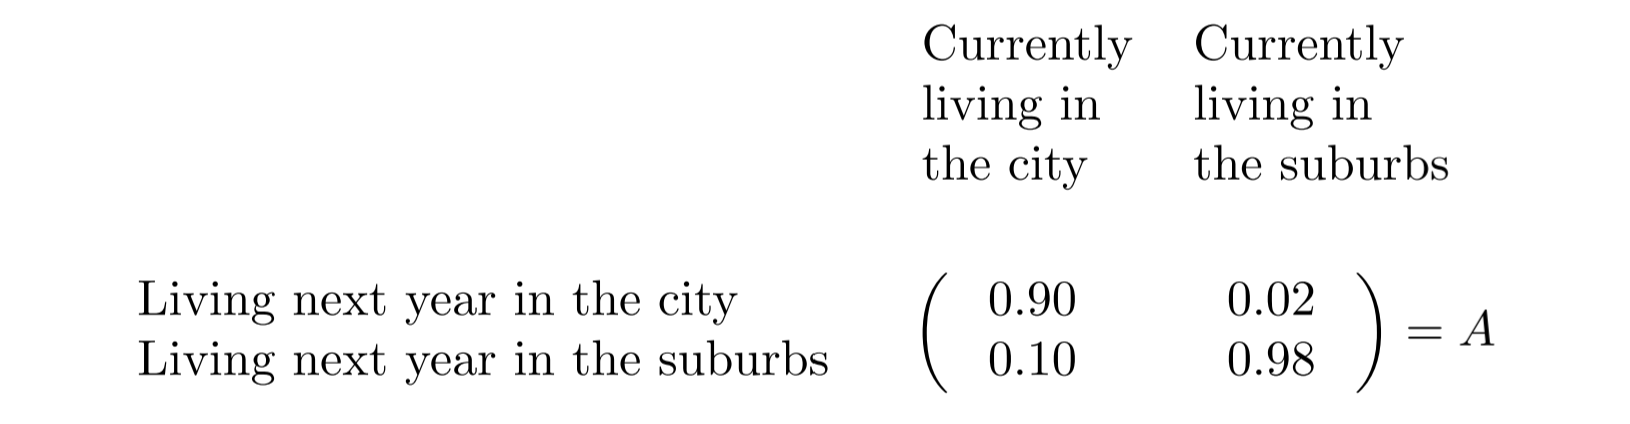
\includegraphics[width=16cm]{images/5-3-city-suburb-movement.png}

For instance, the probability that someone living in the city (on January 1) will be living in the suburbs next year (on January 1) is \(0.10\).
Notice that since the entries of \(A\) are \textbf{probabilities}, they are \textbf{nonnegative}.
Moreover, the \emph{assumption of a constant population} in the metropolitan area requires that \emph{the sum of the entries of each \textbf{column} of \(A\) be \(1\)}.

\begin{additional definition} \label{adef 5.3}
Any square matrix having these two properties (nonnegative entries and columns that sum to \(1\)) is called a \textbf{transition matrix} or a \textbf{stochastic matrix}.
For an arbitrary \(n \X n\) transition matrix \(M\), the rows and columns correspond to \(n\) \textbf{states}, and the entry \(M_{ij}\) represents the probability of moving from state \(j\) to state \(i\) in one \textbf{stage}.
(Note the reversed order of \(ij\)-entry and \(j\)-to-\(i\) movement.)

The \textbf{probability vector} is a vector that has nonnegative entries that sum to \(1\).
Note that each column of a transition matrix is a probability vector.
\end{additional definition}

In our example, there are two states (residing in the city and residing in the suburbs).
So, for example, \(A_{21}\) is the probability of moving from the city to the suburbs in one stage, that is, in one year.
We now determine the probability that a city resident will be living in the suburbs \emph{after \(2\) years}.
There are \emph{two different ways} in which such a move can be made:
remaining in the city for 1 year and then moving to the suburbs, or moving to the suburbs during the first year and remaining there the second year.
(See Figure 5.3.)

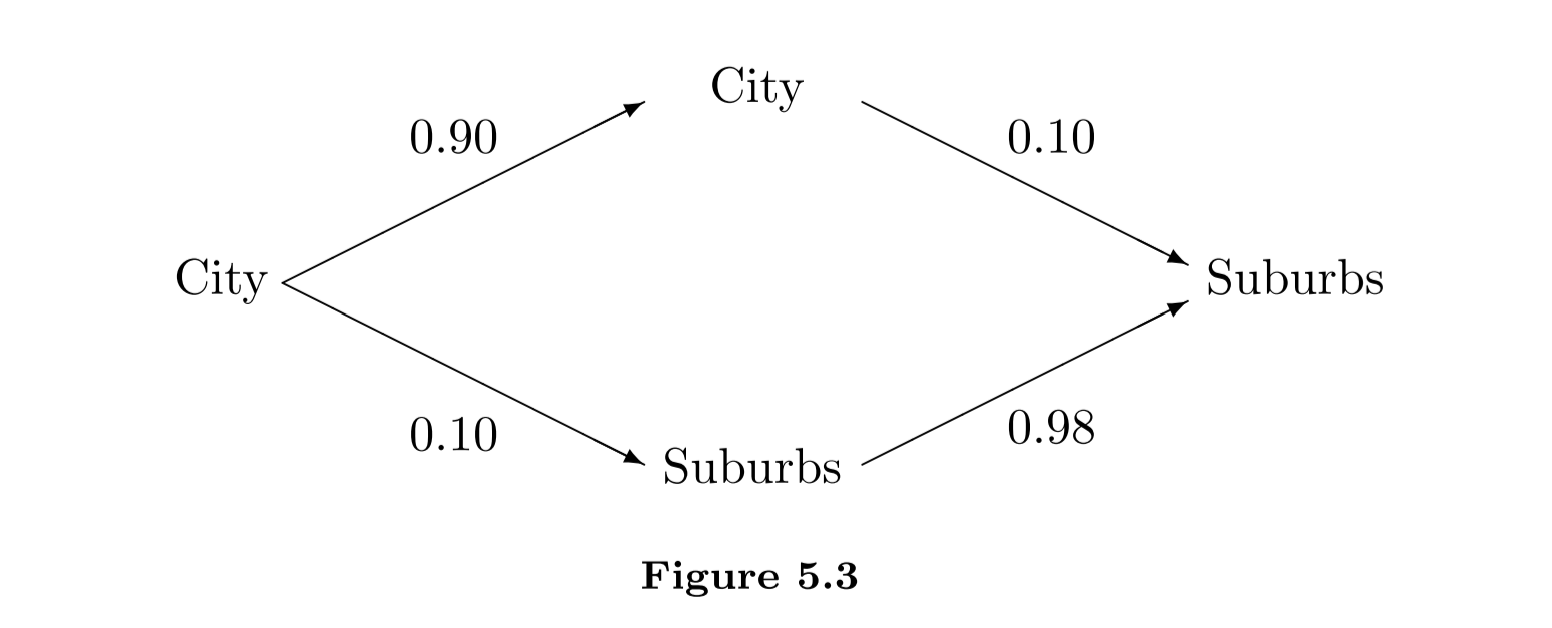
\includegraphics[width=16cm]{images/figure-5-3.png}

The probability that a city dweller remains in the city for the first year is \(0.90\), whereas the probability that the city dweller moves to the suburbs during the first year is \(0.10\).
Hence the probability that a city dweller stays in the city for the first year and then moves to the suburbs during the
second year is the \emph{product} \((0.90)(0.10)\).
Likewise, the probability that a city dweller moves to the suburbs in the first year and remains in the suburbs during the second year is the product \((0.10)(0.98)\).
Thus the probability that a city dweller will be living in the suburbs after 2 years is the \emph{sum of these products}, \((0.90)(0.10) + (0.10)(0.98) = 0.1\).
Observe that this number is \emph{obtained by the same calculation as that which produces \((A^2)_{21}\)},
and hence \((A^2)_{21}\) represents the probability that a city dweller will be living in the suburbs after 2 years.
In general, for any transition matrix \(M\), the entry \((M^m)_{ij}\) represents the probability of moving from state \(j\) to state \(i\) in \(m\) stages.

Suppose additionally that in year 2000, 70\% of the population of the metropolitan area lived in the city and 30\% lived in the suburbs.
We record these data \emph{as a column vector}:

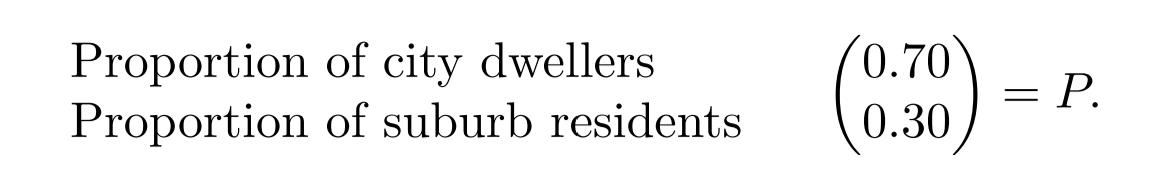
\includegraphics[width=14cm]{images/5-3-city-suburb-prob-vector-1.png}

Notice that the rows of \(P\) correspond to the states of residing in the city and residing in the suburbs, respectively,
and that these \emph{states are listed in the same order as the listing in the transition matrix} \(A\).
Observe also that the column vector \(P\) \emph{contains nonnegative entries that sum to \(1\)};
such a vector is called a \textbf{probability vector}.
In this terminology, \emph{each column of a transition matrix is a probability vector}.
It is often convenient to regard the entries of a transition matrix or a probability vector as \emph{proportions or percentages instead of probabilities}, as we have already done with the probability vector \(P\).

In the vector \(AP = \begin{pmatrix} 0.636 \\ 0.364 \end{pmatrix}\), the first coordinate is the sum \((0.90)(0.70) + (0.02)(0.30)\).
The first term of this sum, \((0.90)(0.70)\), represents the proportion of the 2000 metropolitan population that \emph{remained in the city} during the next year,
and the second term, \((0.02)(0.30)\), represents the proportion of the 2000 metropolitan population that \emph{moved into the city} (from the suburb) during the next year.
Hence the first coordinate of \(AP\) represents the proportion of the metropolitan population that was living in the city in 2001.
Similarly, the second coordinate of \(AP\), represents the proportion of the metropolitan population that was living in the suburbs in 2001.
This argument can be \emph{easily extended} to show that the coordinates of
\[
    A^P = A(AP) = \begin{pmatrix} 0.57968 \\ 0.42032 \end{pmatrix}
\]
represent the proportions of the metropolitan population that were living in each location in 200\RED{2}.
In general, the coordinates of \(A^m P\) represent the \emph{proportion} of the metropolitan population that will be living in the city and suburbs, respectively, after \(m\) stages (\(m\) years after 2000).

From the value of \(AP\) and \(A^2 P\), or just from the value of the entries of \(A\), it seems that the proportion of the population living in cities is getting smaller.
\textbf{Will the city eventually \emph{be depleted} if this trend continues?}
In view of the preceding discussion, it is \emph{natural to define the eventual proportion} of the city dwellers and suburbanites \emph{to be the first and second coordinates, respectively, of} \(\lim_{m \toINF} A^m P\).
We now compute this limit.
It is easily shown that \(A\) is diagonalizable, and so there is an invertible matrix \(Q\) and a diagonal matrix \(D\) such that \(Q^{-1} A Q = D\).
In fact,
\[
    Q = \begin{pmatrix}
        \cfrac{1}{6} & -\cfrac{1}{6} \\ \cfrac{5}{6} & \cfrac{1}{6}
    \end{pmatrix}
    \quad \text{ and }
    D = \begin{pmatrix}
        1 & 0 \\ 0 & 0.88
    \end{pmatrix}.
\]
Therefore (using the process in the proof of \THM{5.13},)
\[
    L = \lim_{m \toINF} A^m = \lim_{m \toINF} Q D^m Q^{-1}) = Q \begin{pmatrix} 1 & 0 \\ 0 & 0 \end{pmatrix} Q^{-1} =
    \begin{pmatrix}
        \cfrac{1}{6} & \cfrac{1}{6} \\ \cfrac{5}{6} & \cfrac{5}{6}
    \end{pmatrix}
\]
Consequently, (by \THM{5.11})
\[
    \lim_{m \toINF} A^m P = LP = \begin{pmatrix}
        \cfrac{1}{6} \\ \cfrac{5}{6}
    \end{pmatrix}
\]
Thus, eventually, \(\frac{1}{6}\) of the population will live in the city and \(\frac{5}{6}\) will live in the suburbs each year.
Note that the vector \(LP\) satisfies \(A (LP) = LP  = 1 \cdot LP\).
Hence \(LP\) is \textbf{both a probability vector} and \textbf{an eigenvector of \(A\)} corresponding \textbf{to the eigenvalue \(1\)}. Since the eigenspace of \(A\) corresponding to the eigenvalue \(1\) is one-dimensional (just by calculation),
there is only one such vector \(L\), that is, the vector that is an eigenvector of \(A\) corresponding to the eigenvalue \(1\) and sums its entries to \(1\) is \emph{unique}.
And \(LP\) is \textbf{independent of the initial choice} of probability vector \(P\).
(See \EXEC{5.3.15}.)
For example, had the 2000 metropolitan population consisted entirely of city dwellers, the
limiting outcome would be the same.

\begin{remark} \label{remark 5.3.4}
In analyzing the city suburb problem, we gave \emph{probabilistic interpretations} of \(A^2\) and \(AP\), showing that \(A^2\) is a transition matrix and \(AP\) is a probability vector.
In fact, the product of any two transition matrices \emph{is} a transition matrix, and the product of any transition matrix and probability vector \emph{is} a probability vector.
A proof of these facts is a simple corollary of the next theorem, which characterizes transition matrices and probability
vectors.
\end{remark}

\begin{theorem} \label{thm 5.14}
Let \(M\) be an \(n \X n\) matrix having \emph{real nonnegative} entries, let \(v\) be a column vector in \(\SET{R}^n\) having nonnegative coordinates, and let \(u \in \SET{R}^n\) be the column vector in which \emph{each coordinate equals \(1\)}.
Then
\begin{enumerate}
\item \(M\) is a transition matrix if and only if \(u^\top M = u^\top\);
\item \(v\) is a probability vector if and only if \(u^\top v = (1)\).
\end{enumerate}
\end{theorem}

\begin{proof}
See \EXEC{5.3.16}.
\end{proof}

\begin{corollary} \label{corollary 5.14.1} \ 

\begin{enumerate}
\item The product of two \(n \X n\) transition matrices is an \(n \X n\) transition matrix.
In particular, any power of a transition matrix is a transition matrix.

\item The product of a transition matrix and a probability vector is a probability vector.
\end{enumerate}
\end{corollary}

\begin{proof}
See \EXEC{5.3.16}.
\end{proof}

\begin{remark} \label{remark 5.3.5}
The city-suburb problem is \emph{an example of a process} in which elements of a set are each \emph{classified as being in one of several fixed states} that \emph{can switch over time}.
In general, such a process is called a \textbf{stochastic process}.
The switching to a particular state is described by a probability, and \emph{in the most general case}, this probability depends on such factors as the state in question, the \emph{time} in question, some or all of the \emph{previous states} in which the object has been (including the current state), and the states that \emph{other objects} are in or have been in.

(For instance, the object could be an American voter, and the state of the object could be his or her preference of political party.
In this example, all four of the factors mentioned above influence the probability that an object is in a particular state at a particular time.)

If, however, the probability that an object in one state \(A\) changes to a different state \(B\) \emph{in a fixed interval of time} depends only on the two states \(A\) and \(B\) (and not on the time, earlier states, or other factors), then the stochastic process is called a \textbf{Markov process}.
If, in addition, the number of possible states is \emph{finite}, then the Markov process is called a \textbf{Markov chain}.
We treated the city suburb example as a two-state Markov chain.
Of course, a Markov process is usually only an idealization of reality because the probabilities involved are almost never constant over time.

Note that some literature defines Markov chain as a Markov process and having \emph{countable} states.
\end{remark}

(Skip another example in page 290 to 292.)

In the preceding two examples, we saw that \(\lim_{m \toINF} A^m P\), where \(A\) is the transition matrix and \(P\) is the initial probability vector of the Markov chain, gives the eventual proportions in each state.
In general, however, \textbf{the limit of powers of a transition matrix need not exist}.
For example, if
\[
    M = \begin{pmatrix} 0 & 1 \\ 1 & 0 \end{pmatrix},
\]
then \(\lim_{m \toINF} M^m\) does not exist because odd powers of \(M\) equal \(M\) and even powers of \(M\) equal \(I\).
The reason that the limit fails to exist is that \textbf{condition (a) of \THM{5.12} does not hold for \(M\)} (\(-1\) is an eigenvalue, but \(-1 \notin S\) where \(S\) is defined in \RMK{5.3.2}).
In fact, it can be shown (see \EXEC{7.2.20}) that \textbf{the only transition matrices} \(A\) such that \(\lim_{m \toINF} A^m\) does not exist are precisely those matrices for which condition (a) of \THM{5.12} fails to hold.

But even if the limit of powers of the transition matrix exists, the computation of the limit may be quite difficult.
(The reader is encouraged to work \EXEC{5.3.6} to appreciate the truth of the last sentence.)
Fortunately, there is a large and important class of transition matrices for which this limit exists and is easily computed -- this is the class of \textbf{regular transition matrices}.

\begin{definition} \label{def 5.11}
A transition matrix is called \textbf{regular} if \emph{some power} of the matrix contains only nonzero (i.e., positive) entries.
\end{definition}

\begin{example} \label{example 5.3.2}
The transition matrix
\[
    \begin{pmatrix} 0.90 & 0.02 \\ 0.10 & 0.98 \end{pmatrix}
\]
of the Markov chain used in the city-suburb problem is clearly regular because each entry is positive.
On the other hand, the transition matrix
\[
    A = \begin{pmatrix}
        1 & 0.4 & 0.1 & 0 \\
        0 & 0.3 & 0.5 & 0 \\
        0 & 0 & 0.2 & 0 \\
        0 & 0.3 & 0.2 & 1
    \end{pmatrix}
\]
is not regular because the first column of \(A^m\) is
\[
    \begin{pmatrix} 1 \\ 0 \\ 0 \\ 0 \end{pmatrix}
\]
for any power \(m\).

Observe that a regular transition matrix \emph{may contain zero entries}.
For example,
\[
    M = \begin{pmatrix} 0.9 & 0.5 & 0 \\ 0 & 0.5 & 0.4 \\ 0.1 & 0 & 0.6 \end{pmatrix}
\]
is regular because every entry of \(M^2\) is positive.
\end{example}

\begin{remark} \label{remark 5.3.6}
The remainder of this section is devoted to proving that, for a \textbf{regular} transition matrix \(A\), the \emph{limit} of the sequence of powers of \(A\) exists and \textbf{has identical columns}.
From this fact, it is easy to compute this limit.
In the course of proving this result, we \emph{obtain some interesting bounds for the magnitudes of eigenvalues of any square matrix}.
These bounds are given in terms of the sum of the absolute values of the rows and columns of the matrix.
The necessary terminology is introduced in the definitions that follow.
\end{remark}

\begin{definition} \label{def 5.12}
Let \(A \in M_{n \X n}(\SET{C})\).
For \(1 \le i, j \le n\), define \(\rho_i(A)\) to be the sum of the \emph{absolute values} of the entries of row \(i\) of \(A\), and define \(\nu(A)\) to be equal to the sum of the absolute values of the entries of column \(j\) of \(A\).
Thus
\[
    \rho_i(A) = \sum_{j = 1}^n \abs{A_{ij}} \quad \text{for} i = 1, 2, ..., n
\]
and
\[
    \nu_j(A) = \sum_{i = 1}^n \abs{A_{ij}} \quad \text{for} j = 1, 2, ..., n.
\]
The \textbf{row sum} of \(A\), denoted \(\rho(A)\), and the \textbf{column sum} of \(A\), denoted \(\nu(A)\), are defined as
\[
    \rho(A) = \max \{ \rho_i(A) : 1 \le i \le n \} \quad \text{ and } \quad \nu(A) = \max \{ \nu_j(A) : 1 \le j \le n \}.
\]
\end{definition}

\begin{example} \label{example 5.3.3}
For the matrix
\[
    A = \begin{pmatrix}
        1 & -\iu & 3-4\iu \\
        -2+\iu & 0 & 6 \\
        3 & 2 & \iu
    \end{pmatrix}
\]
\(\rho_1(A) = 7, \rho_2(A) = 6 + \sqrt{5}, \rho_3(A) = 6, \nu_1(A) = 4 + \sqrt{5}, \nu_2(A) = 3\), and  \(\nu_3(A) = 12\).
Hence \(\rho(A) = 6 + \sqrt{5}\) and \(\nu(A) = 12\).
\end{example}

Our next results show that the \emph{smaller} of \(\rho(A)\) and \(\nu(A)\) is an \textbf{upper bound for the absolute values of eigenvalues of \(A\).} 
In the preceding example, for instance, \(A\) has no eigenvalue with absolute value greater than \(6 + \sqrt{5}\).

To obtain a \emph{geometric view} of the following theorem, we introduce some terminology.
\begin{additional definition}
For an \(n \X n\) matrix \(A\), we define the \(i\)th \textbf{Gershgorin disk} \(C_i\) to be the \emph{disk in the complex plane} with center \(A_{ii}\) and radius \(r_i = \rho_i(A) - \abs{A_{ii}}\);
that is
\[
    C_i = \{ z \in \SET{C} : \abs{z - A_{ii}} \le r_i \}.
\]
\end{additional definition}

For example, consider the matrix
\[
    A = \begin{pmatrix} 1 + 2 \iu & 1 \\ 2 \iu & -3 \end{pmatrix}.
\]
For this matrix, \(C_1\) is the disk with center \(1 + 2\iu\) and radius \(1\), and \(C_2\) is the disk with center \(-3\) and radius \(2\).
(See Figure 5.4)

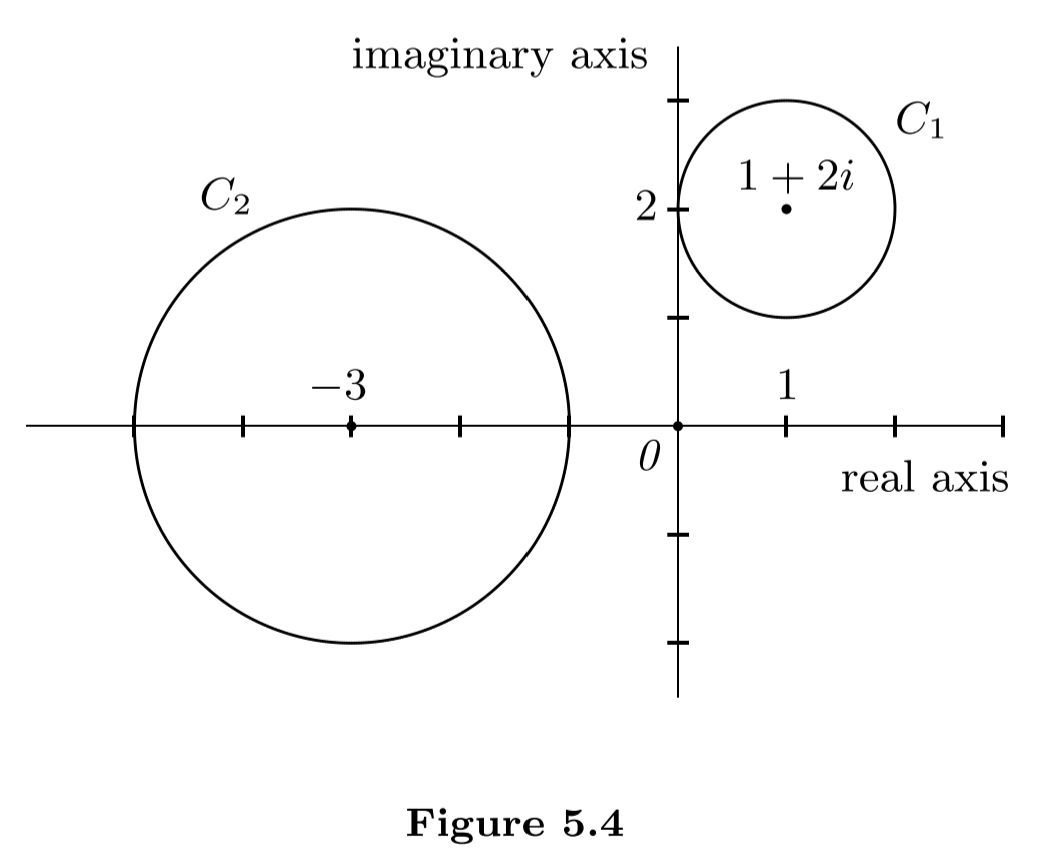
\includegraphics[width=14cm]{images/figure-5-4.png}

Gershgorin's circle theorem, stated below, tells us that all the eigenvalues of \(A\) are located within these two disks.
In particular, we see that \(0\) is \emph{not} an eigenvalue, and hence by \EXEC{5.1.9}(c), \(A\) is invertible.

\begin{theorem} [Gershgorin's Circle Theorem] \label{thm 5.15}
Let \(A \in M_{n \X n}(\SET{C})\).
Then every eigenvalue of \(A\) is contained in a Gersbgorin disk.
\end{theorem}

\begin{proof}
Let \(\lambda\) be an eigenvalue of \(A\) with the corresponding eigenvector
\[
    v = \begin{pmatrix} v_1 \\ v_2 \\ \vdots \\ v_n \end{pmatrix}.
\]
Then \(v\) satisfies the matrix equation \(Av = \lambda v\), which can be written as
\[
    \sum_{j = 1}^n A_{ij} v_j = \lambda v_i \text{for \(1 \le i \le n\)}. \quad \quad \quad \MAROON{(1)}
\]
Suppose that \(v_k\) is a coordinate of \(v\) having the \emph{largest absolute value}; \MAROON{(2)} \quad \quad
note that since \(v\) is an eigenvector, \(v \ne \OV\), hence some coordinate \(v_i\) is nonzero, which implies \(v_k \ne 0\). \MAROON{(3)} \quad \quad
We show that \(\lambda\) \textbf{lies in \(C_k\)}, that is, \(\abs{\lambda - A_{kk}} \le r_k\).
(We will do some trick: multiply \(\abs{v_k}\) in the both sides of this to-be-proved inequality.)
For \(i = k\), it follows from \(\MAROON{(1)}\) that
\begin{align*}
    \abs{v_k}\abs{\lambda - A_{kk}} & = \abs{(v_k)(\lambda - A_{kk})} & \text{by \THM{d.3}(a)} \\
        & = \abs{\lambda v_k - A_{kk} v_k} & \text{of course} \\
        & = \left| \sum_{j = 1}^n A_{kj} v_j - A_{kk} v_k \right| & \text{by \MAROON{(1)}} \\
        & = \left| \sum_{j \ne k} A_{kj} v_j \right| & \text{of course} \\
        & \le \sum_{j \ne k} \abs{ A_{kj} } \abs{ v_j } & \text{by \THM{d.3}(c)} \\
        & \le \sum_{j \ne k} \abs{ A_{kj} } \abs{ v_{\RED{k}} } & \text{by \MAROON{(2)}} \\
        & = \abs{v_k} \sum_{j \ne k} \abs { A_{kj} } & \text{move ``constant'' out of summation} \\
        & = \abs{v_k} r_k. & \text{by def of \(r_k\)}
\end{align*}
Thus we have \(\abs{v_k}\abs{\lambda - A_{kk}} \le \abs{v_k} r_k\).
And since by \MAROON{(3)}, \(\abs{v_k} > 0\), hence (by cancellation law) we have \(\abs{\lambda - A_{kk}} \le r_k\).
\end{proof}

\begin{corollary} \label{corollary 5.15.1}
Let \(\lambda\) be any eigenvalue of \(A \in M_{n \X n}(\SET{C})\).
Then \(\abs{lambda} \le \rho(A)\).
\end{corollary}

\begin{proof}
By Gershgorin's circle theorem, \(\abs{\lambda - A_{kk}} \le r_k\) for some \(k\). \MAROON{(1)} \quad \quad
Hence
\begin{align*}
    \abs{\lambda} & = \abs{(\lambda - A_{kk}) + A_{kk}} & \text{of course} \\
        & \le \abs{\lambda - A_{kk}} + \abs{A_{kk}} & \text{by \THM{d.3}(c)} \\
        & \le r_k + \abs{A_{kk}} & \text{by \MAROON{(1)}} \\
        & = \rho_k(A) & \text{by \DEF{5.12}} \\
        & \le \rho(A). & \text{by definition}
\end{align*}
\end{proof}

\begin{note}
這個\ Corollary 的意義是,eigenvalue 的絕對值會小於等於矩陣的行和。
\end{note}

\begin{corollary} \label{corollary 5.15.2}
Let \(\lambda\) be any eigenvalue of \(A \in M_{n \X n}(\SET{C})\).
Then
\[
    \abs{\lambda} \le \min \{ \rho(A), \nu(A) \}.
\]
\end{corollary}

\begin{proof}
Since \(\abs{\lambda} \le \rho(A)\) by \(1\), it suffices to show that \(\abs{\lambda} \le \nu(A)\).
By \EXEC{5.1.15}, \(\lambda\) is an eigenvalue of \(A^\top\), and so \(\abs{\lambda} \le \rho(A^\top)\) by \CORO{5.15.1}.
But the rows of \(A^\top\) are the columns of \(A\); consequently \(\rho(A^\top) = \nu(A)\).
Therefore \(\abs{\lambda} \nu(A)\).
\end{proof}

The next corollary is immediate from \CORO{5.15.2}
\begin{corollary} \label{corollary 5.15.3}
If \(\lambda\) is an eigenvalue of a \emph{transition} matrix, then \(\abs{\lambda} \le 1\).
(Since each column of a transition matrix sums to \(1\).)
\end{corollary}

\begin{theorem} \label{thm 5.16}
Every \emph{transition} matrix has \(1\) as an eigenvalue.
\end{theorem}

\begin{proof}
Let \(A\) be an \(n \X n\) \emph{transition} matrix, and let \(u \in \SET{R}^n\) be the column vector in which \emph{each coordinate is \(1\)}.
Then \(A^\top u = u\) by \THM{5.14}, and hen\(c\)e \(u\) is an eigenvector of \(A^\top\) corresponding to the eigenvalue \(1\). But since \(A\) and \(A^\top\) have the same eigenvalues, it follows that \(1\) is also an eigenvalue of \(A\).
\end{proof}

Suppose that \(A\) is a transition matrix for which some eigenvector corresponding to the eigenvalue \(1\) \emph{has only nonnegative coordinates}.
Then some multiple of this vector is \emph{a probability vector} \(P\) as well as an eigenvector of \(A\) corresponding to eigenvalue \(1\).
It is interesting to \emph{observe}(i.e. not proved yet) that if \(P\) is the initial probability vector of a Markov chain having \(A\) as its transition matrix, then the Markov chain is \emph{completely static}.
(That is, in particular, \(AP = P\).)
For in this situation, \(A^m P = P\) for every positive integer \(m\); hence the probability of being in each state never
changes.
Consider, for instance, the city suburb problem with
\[
    P = \begin{pmatrix} \cfrac{1}{6} \\ \cfrac{5}{6} \end{pmatrix}.
\]

\begin{theorem} \label{thm 5.17}
Let \(A \in M_{n \X n}(\SET{C})\) be a matrix in which each entry is a positive real number, and let \(\lambda\) be a \emph{complex} eigenvalue of \(A\) such that \(\abs{\lambda} = \rho(A)\).
Then \(\lambda = \rho(A)\) and \(\{ u \}\) is a basis for \(E_{\lambda}\), where \(u \in C^n\) is the column vector in which each coordinate equals \(1\).
\end{theorem}

\begin{note}
That is, given a ``positive'' matrix \(A\), if \(\lambda\) is an eigenvalue and equal to the row sum of \(A\), then \(\lambda\) is in fact also positive.
\end{note}

\begin{proof}
Let \(v\) be an \emph{arbitrary} eigenvector of \(A\) corresponding to \(\lambda\), with coordinates \(v_1, v_2, ..., v_n\).
Suppose that \(v_k\) is the coordinate of \(v\) having the \emph{largest absolute value}, and let \(b = \abs{v_k}\). \MAROON{(b.0)}

Then
\begin{align*}
    \rho(A) b & = \abs{\lambda} b & \text{by supposition} \\
        & = \abs{\lambda} \abs{v_k} & \text{by \MAROON{(b.0)}} \\
        & = \abs{\lambda v_k} & \text{by \THM{d.3}(a)} \\
        & = \left| \sum_{j = 1}^n A_{kj} v_j \right| & \text{in particular from the fact \(Av = \lambda v\)} \\
        &\ \RED{\le} \sum_{j = 1}^n \abs{ A_{kj} v_j } & \text{by \THM{d.3}(c)} \\
        & = \sum_{j = 1}^n \abs{A_{kj}} \abs{v_j} & \text{by \THM{d.3}(a)} \\
        &\ \RED{\le} \sum_{j = 1}^n \abs{A_{kj}} \abs{v_{\RED{k}}} = \sum_{j = 1}^n \abs{A_{kj}} b & \text{since \(\abs{v_k}\) is the largest and \MAROON{(b.0)}} \\
        & = \rho_k(A) b & \text{by def of \(\rho_k(A)\)} \\
        &\ \RED{\le} \rho(A) b \quad \quad \quad \MAROON{(1)} & \text{by def of \(\rho(A)\)}.
\end{align*}
So the three inequalities in the derivation above are actually equalities; that is,
\begin{enumerate}
\item \(\left| \sum_{j = 1}^n A_{kj} v_j \right| \RED{=} \sum_{j = 1}^n \abs{ A_{kj} v_j }\),
\item \(\sum_{j = 1}^n \abs{A_{kj}} \abs{v_j} \RED{=} \sum_{j = 1}^n \abs{A_{kj}} b\), and
\item \(\rho_k(A) b \RED{=} \rho(A)\).
\end{enumerate}

We will see in \EXEC{6.1.15}(b) that (a) holds if and only if all the terms \(A_{kj} v_j (j = 1, 2, ... , n)\) are obtained by multiplying some nonzero complex number \(z\) by nonnegative \textbf{real} numbers.
(That is, intuitively, (a) holds, if and only if all these complex numbers are \textbf{parallel and have same direction} in the complex plane.)
Without loss of generality, we assume that \(\abs{z} = 1\). \MAROON{(b.2)}
Thus there exist nonnegative real numbers \(c_1, c_2, ..., c_n\) such that
\[
    A_{kj} v_j = c_j z. \quad \quad \quad \MAROON{(2)}
\]
By (b) and the assumption (that each entry is a positive real number, so) that \(A_{kj} \ne 0\) for all \(k\) and \(j\), we have
\[
    \abs{v_j} = \abs{v_k} = b \text{ for } j = 1, 2, ..., n. \quad \quad \quad \MAROON{(3)}
\]

%根據假設,所有 \(\abs{v_j}\) 都小於等於 \(\abs{v_k}\)。若這時真的有一個 \(\abs{v_j}\) 是 "小於" \(\abs{v_k}\),則 \(\sum_{j = 1}^k \abs{v_j}\) 就一定小於 \(\sum_{j = 1}^n \abs{v_k} = \sum_{j = 1}^n b\)。連帶的,(b) 會是錯的,矛盾。

Combining \MAROON{(2)} and \MAROON{(3)}, we obtain that for \(j = 1, 2, ..., n\),
\begin{align*}
    b & = \abs{v_k} & \text{by \MAROON{(b.0)}} \\
      & = \left| \frac{c_j}{A_{kj}} z \right| & \text{by \MAROON{(2)}}\\
      & = \left| \frac{c_j}{A_{kj}} \right| \abs{z} = \left| \frac{c_j}{A_{kj}} \right| & \text{by \MAROON{(b.2)}} \\
      & = \frac{c_j}{A_{kj}}, & \text{since \(c_j, A_{kj}\) are nonnegative}
\end{align*}
and therefore, by \MAROON{(2)}, we have \(v_j = \cfrac{c_j}{A_{kj}} z = b z\) for all \(j\).
So
\[
    v = \begin{pmatrix} v_1 \\ v_2 \\ \vdots \\ v_n \end{pmatrix}
    = \begin{pmatrix} bz \\ bz \\ \vdots \\ bz \end{pmatrix}
    = bz \begin{pmatrix} 1 \\ 1 \\ \vdots \\ 1 \end{pmatrix}
    = bzu,
\]
(since \(v\) is arbitrary), hence \(\{ u \}\) is a basis for \(E_{\lambda}\).

Finally, observe that all of the entries of \(A_u\) are positive because the same is true for the entries of both \(A\) and \(u\).
But \(Au = \lambda u\), and hence \(\lambda > 0\).
Therefore, \(\lambda = \abs{\lambda} = \rho(A)\).
\end{proof}

\begin{corollary} \label{corollary 5.17.1}
Let \(A \in M_{n \X n}(\SET{C})\) be a matrix in which each entry is positive, and let \(\lambda\) be an eigenvalue of \(A\) such that \(\abs{\lambda} = \nu(A)\).
Then \(\lambda = \nu(A)\), and the dimension of \(E_{\lambda}\) equals \(1\).
\end{corollary}

\begin{proof}
See \EXEC{5.3.17}.
\end{proof}

\begin{corollary} \label{corollary 5.17.2}
Let \(A \in M_{n \X n}(\SET{C})\) be a \emph{transition matrix} in which each entry is positive, and let \(\lambda\) be any eigenvalue of \(A\) other than \(1\).
Then \(\abs{\lambda} < 1\).
Moreover, the eigenspace corresponding to the eigenvalue \(1\) has dimension \(1\).
\end{corollary}

\begin{proof}
See \EXEC{5.3.17}.
\end{proof}

Our next result extends \CORO{5.17.2} to \emph{regular transition} matrices and thus shows that regular transition matrices satisfy condition (a) of \THM{5.12} and \THM{5.13}.

\begin{theorem} \label{thm 5.18}
Let \(A\) be a \emph{regular transition} matrix, and let \(\lambda\) be an eigenvalue of \(A\).
Then
\begin{enumerate}
\item \(\abs{\lambda} \le 1\).
\item If \(\lambda = 1\), then \(\lambda = 1\), and \(\dim(E_{\lambda}) = 1\).
\end{enumerate}
\end{theorem}

\begin{proof} \ 

\begin{enumerate}
\item This was proved as \CORO{5.15.3}.
\item Since \(A\) is regular, there exists a positive integer \(s\) such that \(A^s\) has only positive entries.
Because \(A\) is a transition matrix and the entries of \(A^s\) are positive, the entries of \(A^{s+1} = A^s(A)\) are positive.
Suppose that \(\abs{\lambda} = 1\).
Then (by \EXEC{5.1.16}(b)) \(\lambda^s\) and \(\lambda^{s+1}\) are eigenvalues of \(A^s\) and \(A^{s + 1}\), respectively, having absolute value \(1\).
So by \CORO{5.17.2}, \(\lambda^s = \lambda^{s+1} = 1\).
Thus \(\lambda = 1\).
Let \(E_{\lambda}\). and \(E'_{\lambda}\) denote the eigenspaces of \(A\) and \(A^s\), respectively, corresponding to \(\lambda = 1\).
Then (of course, trivially, from definition,) \(E_{\lambda} \subseteq E'_{\lambda}\);
and, by \CORO{5.17.2}, \(\dim(E'_{\lambda}) = 1\).
Hence \(E_{\lambda} = E'_{\lambda}\), and \(\dim(E_{\lambda}) = 1\).
\end{enumerate}
\end{proof}

\begin{corollary} \label{corollary 5.18.1}
Let \(A\) be a \emph{regular transition} matrix that is \emph{diagonalizable}.
Then \(\lim_{m \toINF} A^m\) exists.
\end{corollary}

\begin{remark} \label{remark 5.3.7}
The preceding corollary, which follows \emph{immediately from \THM{5.18} and \THM{5.13}}, is not the best possible result.
In fact, it can be shown that (in holy \SEC{7.2}) if \(A\) is a regular transition matrix, then the algebraic multiplicity of \(1\) as an eigenvalue of \(A\) is \(1\).
Thus, by \THM{5.7}, condition (b) of \THM{5.12} is satisfied.
So if \(A\) is a \emph{regular transition} matrix, \textbf{\(\lim_{m \toINF} A^m\) exists regardless of whether \(A\) is or is not diagonalizable}.
As with \THM{5.12}, however, the fact that the algebraic multiplicity of \(\lambda = 1\) as an eigenvalue of \(A\) is \(1\) \textbf{cannot be proved at this time}.
Nevertheless, we state this result here (leaving the proof until \EXEC{7.2.21}) and deduce further facts about \(\lim A^m\) when \(A\) is a regular transition matrix.
\end{remark}

\begin{theorem} \label{thm 5.19}
Let \(A\) be a \textbf{regular transition} matrix.
Then
\begin{enumerate}
\item The multiplicity of \(1\) as an eigenvalue of \(A\) is \(1\).
\item \(\lim_{m \toINF} A^m\) exists.
\item \(L = \lim_{m \toINF} A^m\) is a transition matrix.
\item \(AL = LA = L\).
\item The columns of \(L\) are identical.
In fact, each column of \(L\) is equal to \emph{the unique probability vector} \(v\) that is \emph{also an eigenvector} of \(A\) corresponding to the eigenvalue \(1\).
\item For any probability vector \(w\), \(\lim_{m \toINF} (A^m w) = v\).
\end{enumerate}
\end{theorem}

\begin{proof} \ 

\begin{enumerate}
\item See \EXEC{7.2.21}.
\item This follows from part (a) and \THM{5.18} and \THM{5.12}.

\item By \THM{5.14}, we must show that \(u^\top L = u^\top\).
Now \(A^m\) is a transition matrix by the \CORO{5.14.1}, so
\[
    u^\top L = u^\top \lim_{m \toINF} A^m = \lim_{m \toINF} u^\top A^m = \lim_{m \toINF} u^\top = u^\top,
\]
and it follows that \(L\) is a transition matrix.
\item By \THM{5.11},
\[
    AL = A \lim_{m \toINF} A^m = \lim_{m \toINF} A A^m = \lim_{m \toINF} A^{m + 1} = L.
\]
Similarly, \(LA = L\).

\item Since \(AL = L\) by part(d), each column of \(L\) is an eigenvector of \(A\) corresponding to the eigenvalue \(1\).
(Why? See \THM{2.13}(a).)
Moreover, by part(c), each column of \(L\) is a probability vector.
Thus, by part(a), each column of \(L\) is equal to the unique probability vector \(v\) corresponding to the eigenvalue \(1\) of \(A\).

\item Let \(w\) be any probability vector, and set \(y = \lim_{m \toINF} A^m w = L w\).
Then \(y\) is a probability vector by the \CORO{5.14.1}, and also \(A y = A L w = L w = y\) by part(d).
Hence \(y\) is also an eigenvector corresponding to the eigenvalue \(1\) of A.
So \(y = v\) by part(e).
\end{enumerate}
\end{proof}

\begin{definition}
The vector \(v\) in \THM{5.19}(e) is called the \textbf{fixed probability vector} or \textbf{stationary vector} of the regular transition matrix \(A\).
\end{definition}



\section{Invariant Subspaces and the Cayley-Hamilton Theorem} \label{sec 5.4}

In \SEC{5.1}, we observed that if \(v\) is an eigenvector of a linear operator \(\T\), then \(\T\) maps the span of \(\{ v \}\) into itself.
Subspaces that are mapped into themselves are of great importance in the study of linear operators (see, e.g., \EXEC{2.1.29}--\EXEC{2.1.33}).

\begin{definition} \label{def 5.14}
Let \(\T\) be a linear operator on a vector space \(V\).
A subspace \(W\) of \(V\) is called a \textbf{\(\T\)-invariant subspace} of \(V\) if \(\T(W) \subseteq W\), that is, if
\(\T(v) \in W\) for all \(v \in W\).
\end{definition}

\begin{example} \label{example 5.4.1}
Suppose that \(\T\) is a linear operator on a vector space \(V\).
Then the following subspaces of \(V\) are \(\T\)-invariant:
\begin{enumerate}
\item[1.] \(\{ \OV \}\)
\item[2.] \(V\)
\item[3.] \(\RANGET\)
\item[4.] \(\NULLT\)
\item[5.] \(E_{\lambda}\), for any eigenvalue \(\lambda\) of \(\T\).
\end{enumerate}

For 5., see \EXEC{5.4.3}, for other items, see \EXEC{2.1.29}.
\end{example}

\begin{example} \label{example 5.4.2}
Let \(\T\) be the linear operator on \(\SET{R}^3\) defined by
\[
    \T(a, b, c) = (a + b, b + c, 0).
\]
Then the \(xy\)-plane = \(\{ (x, y, 0): x, y \in \SET{R} \}\) and the \(x\)-axis = \(\{ (x, 0, 0): x \in \SET{R}\}\) are (some examples of) \(\T\)-invariant subspaces of \(\SET{R}^3\).
\end{example}

\begin{additional definition} \label{adef 5.5}
Let \(\T\) be a linear operator on a vector space \(V\), and let \(x\) be a \emph{nonzero} vector in \(V\).
The subspace \(W = \spann(\{ x, \T(x), \T^2(x), ... \})\) is called the \textbf{\(\T\)-cyclic subspace of \(V\) generated by \(x\)}.
It is a simple matter to show that \(W\) is \(\T\)-invariant.

Note that we do not require \(V\) to be finite-dimensional.
\end{additional definition}

\begin{remark} \label{remark 5.4.1}
In fact, \(W\) is the ``smallest'' \(\T\)-\emph{invariant subspace} of \(V\) containing \(x\).
That is, any \(\T\)-invariant subspace of \(V\) containing \(x\) must also contain \(W\) (see \EXEC{5.4.11}).
Cyclic subspaces have various uses.
We apply them in this section to establish the Cayley Hamilton theorem.
In \EXEC{5.4.31}, we outline a method for using cyclic subspaces to \emph{compute the \CPOLY{}} of a linear operator \textbf{without resorting to determinants}.
Cyclic subspaces also play an important role in \CH{7}, where we study matrix representations of non-diagonalizable linear operators.
\end{remark}

\begin{example} \label{example 5.4.3}
Let \(\T\) be the linear operator on \(\SET{R}^3\) defined by
\[
    \T(a, b, c) = (-b + c, a + c, 3c).
\]
We determine the \(\T\)-cyclic subspace generated by \(e_1 = (1, 0, 0)\).
Since
\[
    \T(e_1) = \T(1, 0, 0) = (0, 1, 0) = e_2
\]
and
\[
    \T^2(e_1) = \T(\T(e_1)) = \T(e_2) = (-1, 0, 0) = -e_1,
\]
it follows that
\[
    \spann(\{ e_1, \T(e_1), \T^2(e_1), ... \}) = \spann(\{ e_1, e_2 \}) = \{ (s, t, 0) : s, t \in \SET{R} \}.
\]
\end{example}

\begin{example} \label{example 5.4.4}
Let \(\T\) be the linear operator on \(\mathcal{P}(\SET{R})\) defined by \(\T(f(x)) = f'(x)\).
Then the \(\T\)-cyclic subspace generated by \(x^2\) is (of course!) \(\spann(\{ x^2, 2x, 2 \}) = \mathcal{P}_2(\SET{R})\).
\end{example}

\begin{remark} \label{remark 5.4.2}
The existence of a \(\T\)-invariant subspace provides the opportunity to define a new linear operator \textbf{whose domain is this subspace}.
If \(\T\) is a linear operator on \(V\) and \(W\) is a \(\T\)-invariant subspace of \(V\), then the \emph{restriction} \(\T_W\) of \(\T\) to \(W\) (see Appendix B, page 545) is a mapping \emph{from \(W\) to \(W\)}, and it follows that \(\T_W\) is a linear operator on \(W\) (see \EXEC{5.4.7}, or \EXEC{2.1.30}).
As a linear operator, \(\T_W\) \emph{inherits certain properties} from its parent operator \(\T\).
The following result illustrates one way in which the two operators are linked.
\end{remark}

\begin{theorem} \label{thm 5.20}
Let \(\T\) be a linear operator on a finite-dimensional vector space \(V\), and let \(W\) be a \(\T\)-invariant subspace of \(V\).
Then the \CPOLY{} of \(\T_W\) \textbf{divides} the \CPOLY{} of \(\T\).
\end{theorem}

\begin{proof}
Choose an ordered basis \(\gamma = \{ v_1, v_2, ..., v_k \}\) \emph{for \(W\)}, and \emph{extend} it to an ordered basis \(\beta = \{ v_1, v_2, ... v_k, v_{k + 1}, ..., v_n \}\) for \(V\).
Let \(A = [\T]_{\beta}\) and \(B_1 = [\T_W]_{\gamma}\).
Then, by \EXEC{5.4.12}, \(A\) can be written in the form
\[
    A = \begin{pmatrix}
        \RED{B_1} & B_2 \\ O & B_3
    \end{pmatrix}.
\]
Let \(f(t)\) be the \CPOLY{} of \(\T\) and \(g(t)\) the \CPOLY{} of \(\T_W\).
Then
\[
    f(t) = \det(A - tI_n) = \begin{pmatrix} B_1 - t I_{\RED{k}} & B_2 \\ O & B_3 - t I_{\RED{n - k}} \end{pmatrix}
    = g(t) \cdot \det(B_3 - t I_{n - k})
\]
by \EXEC{4.3.21}.
Thus \(g(t)\) divides \(f(t)\).
\end{proof}

\begin{example} \label{example 5.4.5}
Let \(\T\) be the linear operator on \(\SET{R}^4\) defined by
\[
    \T(a, b, c, d) = (a + b + 2c - d, b + d, 2c - d, c + d),
\]
and let \(W = \{ (t, s, 0, 0) : t, s \in \SET{R} \}\).
Observe that \(W\) is a \(\T\)-invariant subspace of \(\SET{R}^4\) because, for any vector \((a, b, 0, 0) \in W\),
\[
    \T(a, b, 0, 0) = (a + b, b, 0, 0) \in W.
\]
Let \(\gamma = \{ e_1, e_2 \}\), which is an ordered basis for \(W\).
Extend \(\gamma\) to the \emph{standard} ordered basis \(\beta\) for \(\SET{R}^4\).
Then
\[
    B_1 = [\T_W]_{\gamma} = \begin{pmatrix} 1 & 1 \\ 0 & 1 \end{pmatrix}
    \quad \text{ and } \quad
    A = [\T]_{\beta} = \begin{pmatrix} 1 & 1 & 2 & -1 \\ 0 & 1 & 0 & 1 \\ 0 & 0 & 2 & -1 \\ 0 & 0 & 1 & 1 \end{pmatrix}
\]
in the notation of \THM{5.20}.
Let \(f(t)\) be the \CPOLY{} of \(\T\) and \(g(t)\) be the \CPOLY{} of \(\T_W\).
Then
\begin{align*}
    f(t) & = \det(A - tI_4) = \det \begin{pmatrix} 1-t & 1 & 2 & -1 \\ 0 & 1-t & 0 & 1 \\ 0 & 0 & 2-t & -1 \\ 0 & 0 & 1 & 1-t \end{pmatrix} & \text{by definition} \\
         & = \det \begin{pmatrix} 1-t & 1 \\ 0 & 1-t \end{pmatrix} \cdot \det \begin{pmatrix} 2-t & -1 \\ 1 & 1-t \end{pmatrix} & \text{by \EXEC{4.3.21}} \\
         & = g(t) \cdot \det \begin{pmatrix} 2-t & -1 \\ 1 & 1-t \end{pmatrix} & \text{by \THM{5.20}}
\end{align*}
\end{example}

\begin{remark} \label{remark 5.4.3}
In view of \THM{5.20}, we may use the \CPOLY{} of \(T_W\) to \emph{gain information} about the \CPOLY{} \emph{of \(\T\) itself}.
In this regard, cyclic subspaces are useful because the \CPOLY{} of the restriction of a linear operator \(\T\) to a cyclic subspace is \emph{readily computable}.
(See the theorem below.)
\end{remark}

\begin{theorem} \label{thm 5.21}
Let \(\T\) be a linear operator on a \textbf{finite}-dimensional vector space \(V\), and let \(W\) denote the \(\T\)-cyclic subspace of \(V\) generated by a nonzero vector \(v \in V\).
Let \(k = \dim(W)\).
Then
\begin{enumerate}
\item \(\beta = \{ v, \T(v), \T^2(v), ..., \T^{\RED{k - 1}}(v) \}\) is a \textbf{basis} for \(W\).
\item If \(\T_{\RED{k}}(v) = -a_0 v - a_1 \T(v) - ... - a_{k - 1} \T^{k - 1}(v) \), then the \CPOLY{} oF \(\T_W\) is \(f(t) = (-1)^k (t^k + a_{k - 1} t^{k-1} + ... + a_1 t + a_0).\).

(That is, If we write \(\T_{\RED{k}}(v)\) as a linear combination \(\beta\), but without loss of generality and a negative sign in these coefficient \(a_i\), we can derive the \CPOLY{} of \(\T_W\) use these coefficients \(a_i\).)
\end{enumerate}
\end{theorem}

\begin{proof} \ 

\begin{enumerate}
\item Since \(v \ne \OV\), the set \(\{ v \}\) is \LID{}.
Let \(j\) be the \emph{largest positive} integer for which
\[
    \beta = \{ v, \T(v), ..., \T^{j - 1}(v) \}
\]
is linearly independent.
Such \(j\) must exist since \(V\) is finite-dimensional (hence any \LID{} set must be finite).
Let \(Z = \spann(\beta)\).
Then \(\beta\) is a generating set for \(Z\) and is \LID{}, hence is a basis for \(Z\).
Furthermore, since by definition of \(j\), \(\beta \cup \{ \T^j(v) \}\) is \LDP{}, \(\T^j(v) \in \spann(\beta)\) by \THM{1.7}.
That is, \(\T^j(v) \in Z\).
We use this information to show that \(Z\) is a \(\T\)-invariant subspace of \(V\).

Let \(w \in Z\).
Since \(w\) is a linear combination of the vectors of \(\beta\), there exist scalars \(b_0, b_1, ..., b_{j - 1}\) such that
\[
    w = b_0 v + b_1 \T(v) + ... + b_{j - 1} \T^{j - 1}(v),
\]
and hence (by applying \(\T\) on both sides,)
\begin{align*}
    \T(w) & = \T(b_0 v + b_1 \T(v) + ... + b_{j - 1} \T^{j - 1}(v)) \\
          & = b_0 \T(v) + b_1 \T^2(v) + ... + b_{j - 2} \T^{\RED{j - 1}}(v) + b_{j - 1} \T^{\RED{j}}(v), & \text{since \(\T\) is linear}
\end{align*}
where \(\T(v), ..., \T^{\RED{j - 1}}(v)\) belong to the bases \(\beta\), and \(\T^{\RED{j}}(v) \in Z\), thus \(\T(w)\) is still a linear combination of vectors in \(Z\), and hence belong to \(Z\).
So \(Z\) is \(\T\)-invariant.
Furthermore, \(v \in Z\) (since \(v \in \beta\)).
By \EXEC{5.4.11}, \(W\) is the \emph{smallest} \(\T\)-invariant subspace of \(V\) that contains \(v\), so that \(W \subseteq Z\).
Clearly, \(Z \subseteq W\) (since \(Z = \spann(\{ v, \T(v), ..., \T^{j - 1}(v) \})\) but \(W = \spann(\{ v, \T(v), ... \})\)), and so we conclude that \(Z = W\).
It follows that \(\beta\) is a basis for \(W\), and therefore \(\dim(W) = j\).
Thus \(j = k\).
This proves (a).

\item Now view \(\beta\) (from part(a)) as an ordered basis for \(W\).
Let \(a_o, a_1, ..., a_{k_1}\) be the scalars such that
\[
    a_0 v + a_1 \T(v) + ... + a_{k - 1} \T^{k - 1} (v) + \RED{\T^k(v)} = \OV. \quad \quad \quad \MAROON{(1)}
\]
(Note that this is \emph{not} a linear combination of vectors in \(\beta\).)
Observe that since
\begin{align*}
    \T(v) & = 0 \cdot v + 1 \cdot \T(v) + 0 \cdot \T^2(V) + ... + 0 \cdot \T^{k - 1}(v) \\
    \T(\T(v)) & = 0 \cdot v + 0 \cdot \T(v) + 1 \cdot \T^2(V) + ... + 0 \cdot \T^{k - 1}(v) \\
    \vdots \\
    \T(\T^{k - 2})(v) & = 0 \cdot v + 0 \cdot \T(v) + 0 \cdot \T^2(V) + ... + 1 \cdot \T^{k - 1}(v) \\
    \T(\T^{k - 1}(v)) & = \T^k(v) = -a_0 \cdot v -a_1 \cdot \T(v) - a_2 \cdot \T^2(v) - ... - a_{k - 1} \T^{k - 1}(v),
\end{align*}
We have
\[
    [\T_W]_{\beta} = \begin{pmatrix}
        0 & 0 & 0 & ... & 0 & -a_0 \\
        1 & 0 & 0 & ... & 0 & -a_1 \\
        0 & 1 & 0 & ... & 0 & -a_2 \\
        \vdots & \vdots & \ddots & & 0 & \vdots \\
        0 & 0 & 0 & & 1 & -a_{k - 1}
    \end{pmatrix},
\]
which has the \CPOLY{}
\[
    f(t) = (-1)^k (t^k + a_{k - 1} t^{k-1} + ... + a_1 t + a_0)
\]
by \EXEC{5.4.19}.
Thus \(f(t)\) is the \CPOLY{} of \(\T_W\), proving (b).
\end{enumerate}
\end{proof}

\begin{example} \label{example 5.4.6}
Let \(\T\) be the linear operator of \EXAMPLE{5.4.3}, and let \(W = \spann(\{ e_1, e_2 \})\), the \(\T\)-cyclic subspace generated by \(e_1\).
We compute the characteristic polynomial \(f(t)\) of \(\T_W\) in two ways: by means of \THM{5.21} and by means of determinants.
\begin{enumerate}
\item \emph{By means of \THM{5.21}}.
From \EXAMPLE{5.4.3}, we know that \(\{ e_1, e_2\}\) is a \textbf{cycle}(\TODOREF{this term seem to be defined in \CH{7}}) that generates \(W\), hence \(\dim(W) = \RED{2}\), hence from \THM{5.21}(a), \(\{ e_1, \T(e_1) \}\) is a basis for \(W\);
in particular, by that example, that set is in fact equal to \(\{ e_1, e_2 \}\).
Also from that example, we have \(\T^{\RED{2}}(e_1) = -e_1\).
And from this equation, we have
\[
    1 \cdot e_1 + 0 \cdot \T(e_1) + \T^{\RED{2}}(e_1) = 0.
\]
Therefore, by \THM{5.21}(b),
\[
    f(t) = (-1)^{\RED{2}} (1 + 0t + t^2) = t^2 + 1.
\]

\item By means of determinants, Let \(\beta = \{ e_1, e_2 \}\), which (by that example) is an ordered basis for \(W\).
Since \(\T(e_1) = e_2\) and \(\T(e_2) = -e_1\), we have
\[
    [\T_W]_{\beta} = \begin{pmatrix} 0 & -1 \\ 1 & 0 \end{pmatrix}.
\]
and therefore
\[
    f(t) = \det \begin{pmatrix} -t & -1 \\ 1 & -t \end{pmatrix} = t^2 + 1.
\]
\end{enumerate}
\end{example}

\subsection{The Cayley-Hamilton Theorem} \label{sec 5.4.1}
As an illustration of the importance of \THM{5.21}, we prove a well-known result that is used in \CH{7}.
The reader should refer to \DEF{e.3} for the definition of \(f(\T)\), where \(\T\) is a linear operator and \(f(x)\) is a polynomial.

\begin{theorem} [Cayley-Hamilton] \label{thm 5.22}
Let \(\T\) be a linear operator on a \emph{finite}-dimensional vector space \(V\), and let \(f(t)\) be the \CPOLY{} of \(\T\).
Then \(f(\T) = \TZERO\), \textbf{the zero transformation}.
That is, \(\T\) ``satisfies'' its characteristic equation.
\end{theorem}

\begin{proof}
We show that \(f(\T)(v) = \OV\) for all \(v \in V\).
This is obvious if \(v = \OV\) because \(f(\T)\) is linear(see \THM{e.3}(a)); so suppose that \(v \ne \OV\).
Let \(W\) be the \(\T\)-cyclic subspace generated by \(v\), and suppose that \(\dim(W) = k\).
By definition of \(\T\)-cyclic, \(\T^k(v) \in W\).
And by \THM{5.21}(a), \(\{ v, \T(v), ..., \T^{k - 1}(v) \}\) is a basis for \(W\), hence there exist scalars \(a_0, a_1, ..., a_{k-1}\) such that
\[
    a_0 v + a_1 \T(v) + ... + a_{k - 1} \T^{k - 1}(v) = -\RED{\T^k(v)},
\]
or
\[
    a_0 v + a_1 \T(v) + ... + a_{k - 1} \T^{k - 1}(v) + \RED{\T^k(v)} = \OV. \quad \quad \quad \MAROON{(1)}
\]
Hence, \THM{5.21}(b) implies that
\[
    g(t) = (-1)^k (a_0 + a_1 t + ... + a_{k - 1} t^{k - 1} + t^k) \quad \quad \quad \MAROON{(2)}
\]
is the \CPOLY{} of \(\T_W\).
Combining these two equations yields
\begin{align*}
    g(\T)(v) & = (-1)^k (a_0 \ITRANV{} + a_1 \T + ... + a_{k - 1} \T^{k - 1} + \T^k)(v) & \text{by \DEF{e.3} and \MAROON{(2)}} \\
        & = (-1)^k [ a_0 \ITRANV{}(v) + a_1\T(v) + ... + a_{k - 1} \T^{k - 1}(v) + \T^k(v) ] & \text{since function \(+, \cdot\) is linear} \\
        & = (-1)^k [ a_0 v + a_1\T(v) + ... + a_{k - 1} \T^{k - 1}(v) + \T^k(v) ] & \text{of course} \\
        & = (-1)^k \cdot \OV & \text{by \MAROON{(1)}} \\
        & = \OV. \quad \MAROON{(3)} & \text{of course}
\end{align*}
By \THM{5.20}, \(g(t)\) divides \(f(t)\); hence there exists a polynomial \(q(t)\) such that \(f(t) = q(t)g(t)\). \MAROON{(4)}

So
\begin{align*}
    f(\T)(v) & = q(\T)g(\T)(v) & \text{by \MAROON{(4)} and \DEF{e.3}} \\
             & = q(\T)(g(\T)(v)) & \text{by def of function composition} \\
             & = q(\T)(\OV) & \text{by \MAROON{(3)}} \\
             & = \OV. & \text{since \(q(\T)\) is also linear by \THM{e.3}(a)}
\end{align*}
So in all cases, \(f(\T)(v) = \OV\) for arbitrary \(v\), as desired.
\end{proof}

\begin{example} \label{example 5.4.7}
Let \(\T\) be the linear operator on \(\SET{R}^2\) defined by \(\T(a, b) = (a + 2b, -2a + b)\), and let \(\beta = \{ e_1, e_2 \}\).
Then
\begin{align*}
    A = \begin{pmatrix} 1 & 2 \\ -2 & 1 \end{pmatrix},
\end{align*}
where \(A = [\T]_{\beta}\).
The \CPOLY{} of \(\T\) is, therefore
\[
    f(t) = \det(A - tI) = \det \begin{pmatrix} 1-t & 2 \\ -2 & 1-t \end{pmatrix} = t^2 - 2t + 5.
\]
It is easily verified that \(\TZERO = f(\T) = \T^2 - 2\T + 5\ITRANV{}\).
Similarly,
\[
    f(A) = A^2 - 2A + 5I =
    \begin{pmatrix} -3 & 4 \\ -4 & -3 \end{pmatrix}
    + \begin{pmatrix} -2 & -4 \\ 4 & -2 \end{pmatrix}
    + \begin{pmatrix} 5 & 0 \\ 0 & 5 \end{pmatrix}
    = \begin{pmatrix} 0 & 0 \\ 0 & 0 \end{pmatrix}.
\]
\end{example}

\EXAMPLE{5.4.7} suggests the following result.

\begin{corollary} [Cayley-Hamilton Theorem for Matrices] \label{corollary 5.22.1}
Let \(A\) be an \(n \X n\) matrix, and let \(f(t)\) be the \CPOLY{} of \(A\).
Then \(f(A) = O\), the \(n \X n\) zero matrix.
\end{corollary}

\begin{proof}
We have to show \(f(A) v = \OV\) for all \(v \in F^n\) and conclude \(f(A) = O\).
Let \(\beta\) be the \emph{standard} ordered basis for \(F^n\), then by \THM{2.15}(a), \([\LMTRAN_A]_{\beta} = A\), and (by \DEF{5.4}) \(f(t)\) is equal to the \CPOLY{} of \(\LMTRAN_A\).
Without loss of generality, let \(f(t) = a_0 + a_1 t + ... + a_n t^n\). \MAROON{(1)}

We have
\begin{align*}
    f(A) v & = [a_0 I + a_1 A + ... + a_n A^n](v) & \text{by \MAROON{(1)} and \DEF{e.3}} \\
           & = (a_0 I)(v) + (a_1 A)(v) + ... + (a_n A^n)(v) & \text{by \THM{2.12}} \\
           & = a_0 [\ITRANV{}]_{\beta} (v) + a_1 [\LMTRAN_A]_{\beta} (v) + ... + a_n [(\LMTRAN_A)^n] (v) & \text{by \THM{2.15} and \THM{2.11}} \\
           & = [\left( a_0 \ITRANV{} + a_1 \LMTRAN_A + ... + a_n (\LMTRAN_A)^n \right) (v)]_{\beta} & \text{just by \CH{2}, :P} \\
           & = [\TZERO(v)]_{\beta} = [\OV]_{\beta} & \text{by \THM{5.22}} \\
           & = \OV & \text{since \(\OV \in F^n\)}
\end{align*}
\end{proof}

\subsection{Invariant Subspaces and Direct Sums} \label{sec 5.4.2}
This subsection uses optional material on direct sums from subsection \ref{sec 5.2.3}.

It is useful to decompose a finite-dimensional vector space \(V\) into a \emph{direct sum} of as many \(\T\)-\textbf{invariant} subspaces as possible because the behavior of \(\T\) on \(V\) can be inferred from its behavior on the direct summands.
For example, \(\T\) is diagonalizable if and only if \(V\) can be decomposed into a direct sum of \textbf{one-dimensional} \(\T\)-invariant subspaces (see \EXEC{5.4.35}).
In \CH{7}, we consider \emph{alternate ways} of decomposing \(V\) into direct sums of \(\T\)-invariant subspaces if \(\T\) is not diagonalizable.
We proceed to gather a few facts about direct sums of \(\T\)-invariant subspaces that are used in \SEC{7.4}.
The first of these facts is about \CPOLY{}s.

\begin{theorem} \label{thm 5.23}
Let \(\T\) be a linear operator on a finite-dimensional vector space \(V\), and suppose that \(V = W_1 \oplus W_2 \oplus ... \oplus W_{\RED{k}}\), where \(W_i\) is a \(\T\)-\textbf{invariant} subspace of \(V\) for each \(i (1 \le i \le k)\).
Suppose that \(f_i(t)\) is the \CPOLY{} of \(T_{W_i} (1 \le i \le k)\).
Then \(f_1(t) \cdot f_2(t) \cdot ... \cdot f_k(t)\) is the \CPOLY{} of \(\T\).
\end{theorem}

\begin{proof}
The proof is by mathematical induction on \(\RED{k}\).
In what follows, \(f(t)\) denotes the \CPOLY{} of \(\T\).
Suppose first that \(k = 2\).
(That is, \(V = W_1 \oplus W_2\) where \(W_1, W_2\) are \(\T\)-invariant subspaces of \(V\).)
Let \(\beta_1\) be an ordered basis for \(W_1\), \(\beta_2\) an ordered basis for \(W_2\), and \(\beta = \beta_1 \cup \beta_2\).
Then \(\beta\) is an ordered basis for \(V\) by \THM{5.9}(d).
Let \(A = [\T]_{\beta}\), \(B_1 = [\T_{W_1}]_{\beta_1}\) and \(B_2 = [\T_{W_2}]_{\beta_2}\).
By \EXEC{5.4.33}, it follows that
\[
    A = \begin{pmatrix}
        B_1 & O \\
        O' & B_2
    \end{pmatrix},
\]
where \(O\) and \(O'\) are zero matrices of the appropriate sizes.
Then, without loss of generality that each \(I\) denotes identity matrix of the appropriate size, we have
\begin{align*}
    f(t) & = \det(A - tI) & = \begin{pmatrix} B_1 - tI & O \\ O' & B_2 - tI \end{pmatrix}\\
         & = \det(B_1 - tI) \cdot det(B_2 - tI) & \text{by \EXEC{4.3.21}} \\
         & = f_1(t), \cdot f_2(t) & \text{by definition}
\end{align*}
proving the result for \(k = 2\).

Now assume that the theorem is valid for \(k - 1\) summands, where \(k - 1 \ge 2\).
(That is, given any linear operator \(\T\), and suppose that \(V = W_1 \oplus W_2 \oplus ... \oplus W_{\RED{k - 1}}\), where \(W_i\) is a \(\T\)-\textbf{invariant} subspace of \(V\) for each \(i (1 \le i \le k)\), and \(f_i(t)\) is the \CPOLY{} of \(T_{W_i} (1 \le i \le k)\).
Then \(f_1(t) \cdot f_2(t) \cdot ... \cdot f_{k - 1}(t)\) is the \CPOLY{} of \(\T\).)

And suppose that \(V\) is a direct sum of \(k\) \(\T\)-\textbf{invariant}\RED{*} subspaces, say,
\[
    V = W_1 \oplus W_2 \oplus ... \oplus W_{k - 1} \oplus W_k.
\]
Let \(W = W_1 + W_2 + ... + W_{k - 1}\).
It is \emph{easily verified} that \(W\) is \(\T\)-invariant and that \(V = W \oplus W_k\).
So by the case for \(k = 2\), \(f(t) = g(t) \cdot f_k(t)\), where \(g(t)\) is the \CPOLY{} of \(\T_W\).

\RED{**}And clearly, \(W_i\) are subspace of \(W\), and furthermore, \(W_i\) is a \(\T_{\RED{W}}\)-invariant subspace of \(W\).
Also, clearly, \(W = W_1 \oplus W_2 ... \oplus W_{k - 1}\).
Therefore, all conditions of induction hypothesis are satisfied, hence \(g(t) = f_1(t) \cdot f_2(t) \cdot ... \cdot f_{k - 1}(t)\) by the induction hypothesis.
Combining these facts, we have \(f(t) = g(t) \cdot f_k(t) = f_1(t) \cdot f_2(t) \cdot ... \cdot f_{k - 1}(t) \cdot f_k(t)\).
\end{proof}

\begin{note}
\RED{*}: The proof in the book for the case \(k\) does not say that \(W_1, ..., W_k\) are \(\T\)-invariant, but it seems that they need to be \(\T\)-invariant.

\RED{**}: In my opinion, the usage of the induction hypothesis in the book is too vague to be correct.
\end{note}

\begin{remark} \label{remark 5.4.4}
As an illustration of \THM{5.23}, suppose that \(\T\) is a diagonalizable linear operator on a \emph{finite}-dimensional vector space \(V\) with distinct eigenvalues \(\lambda_1, \lambda_2, ..., \lambda_k\).
By \THM{5.10}, (since \(\T\) is diagonalizable,) \(V\) is a direct sum of the \emph{eigenspaces} of \(\T\).
Since each eigenspace \emph{is} \(\T\)-invariant (see \EXAMPLE{5.4.1}), we may view this situation in the context of \THM{5.23}.
(That is, we have \(E_{\lambda_1}, ..., E_{\lambda_k}\) as \(\T\)-invariant subspaces and \(V = E_{\lambda_1} \oplus ... \oplus E_{\lambda_k}\).
For each eigenvalue \(\lambda_i\), the \emph{restriction} of \(\T\) to \(E_{\lambda_i}\), has characteristic polynomial \((\lambda - t)^{m_i}\), where \(m_i\) is the dimension of \(E_{\lambda_i}\).
(why \((\lambda - t)^{m_i}\)? Given any basis \(\beta_i\) for \(E_{\lambda_i}\), then \([\T_{E_{\lambda_i}}]_{\beta}\) is a diagonal matrix such that each diagonal entry is \(\lambda_i\), since each vector in the basis is scaled \(\lambda_i\) times by \(\T_{E_{\lambda_i}}\).)
By \THM{5.23}, the characteristic polynomial \(f(t)\) of \(\T\) is the product
\[
    f(t) = (\lambda_1 - t)^{m_1} (\lambda_2 - t)^{m_2} ... (\lambda_k - t)^{m_k}.
\]
It follows that the algebraic multiplicity of each eigenvalue is equal to the dimension of the corresponding eigenspace, as expected.
\end{remark}

\begin{example} \label{example 5.4.8}
Let \(\T\) be the linear operator on \(\SET{R}^4\) defined by
\[
    \T(a, b, c, d) = (2a - b, a + b, c - d, c + d),
\]
and let \(W_1 = \{(s, t, 0, 0): s,t \in \SET{R}\}\) and \(W_2 = \{(0, 0, s, t): s,t \in \SET{R}\}\).
Notice that \(W_1\) and \(W_2\) are each \(\T\)-invariant and that \(\SET{R}^4 = W_1 \oplus W_2\).
Let \(\beta_1 = \{ e_1, e_2 \}\), \(\beta_2 = \{ e_3, e_4 \}\), and \(\beta = \beta_1 \cup \beta_2 = \{ e_1, e_2, e_3, e_4 \}\).
Then \(\beta_1\) is an ordered basis for \(W_1\), \(\beta_2\) is an ordered basis for \(W_2\), and \(\beta\) is an ordered basis for \(\SET{R}^4\).
Let \(A= [\T]_{\beta}, B_1 = [\T_{W_1}]_{\beta_1}\) and \(B_2 = [\T_{W_2}]_{\beta_2}\).
Then
\[
    B_1 = \begin{pmatrix} 2 & -1 \\ 1 & 1 \end{pmatrix}, \quad
    B_2 =\begin{pmatrix} 1 & -1 \\ 1 & 1 \end{pmatrix}
\]
and
\[
    A = \begin{pmatrix} B_1 & O \\ O & B_2 \end{pmatrix}
    = \begin{pmatrix}
        2 & -1 & 0 & 0 \\
        1 & 1 & 0 & 0 \\
        0 & 0 & 1 & -1 \\
        0 & 0 & 1 & 1
    \end{pmatrix}
\]
Let \(f(t), f_1(t)\), and \(f_{2}(t)\) denote the \CPOLY{} of \(\T, \T_{W_1}\), and \(\T_{W_2}\), respectively.
Then by \THM{5.23},
\[
    f(t) = \det(A - tI) = \det(B_1 - tI) \cdot \det(B_2 - tI) = f_1(t) \cdot f_2(t).
\]
\end{example}

The matrix \(A\) in \EXAMPLE{5.4.8} can be obtained by \emph{joining} the matrices \(B_1\) and \(B_2\) in the manner explained in the next definition.

\begin{definition} \label{def 5.15}
Let \(B_1 \in M_{m \X m}(F)\), and let \(B_2 \in M_{n \X n}(F)\).
We define the direct sum of \(B_1\) and \(B_2\), (that is, the ``direct sum of two matrices'') denoted \(B_1 \oplus B_2\), as the \((m + n) \X (m + n)\) matrix \(A\) such that
\begin{equation*}
    A_{ij} = \begin{cases}
        (B_1)_{ij} & \text{ for } 1 \le i, j \le m \\
        (B_2)_{(i - m), (j - m)} & \text{ for } m + 1 \le i, j \le m + n \\
        0 & \text{ otherwise. }
    \end{cases}
\end{equation*}

If \(B_1, B2, ..., B_k\) are square matrices with entries from \(F\), then we define the \textbf{direct sum} of \(B_1, B_2, ..., B_k\) \emph{recursively} by
\[
    B_1 \oplus B_2 \oplus ... \oplus B_k = (B_1 \oplus B_2 \oplus ... \oplus B_{k - 1}) \oplus B_k.
\]
If \(A = B_1 \oplus B_2 \oplus ... \oplus B_k\), then we often writ
\[
    A = \begin{pmatrix}
        B_1 & O & ... & O \\
        O   & B_2 & ... & O \\
        \vdots & \vdots & & \vdots \\
        O & O & \vdots & B_k
    \end{pmatrix}.
\]
\end{definition}

\begin{example} \label{example 5.4.9}
Let
\[
    B_1 = \begin{pmatrix} 1 & 2 \\ 1 & 1  \end{pmatrix},
    \quad B_2 = \begin{pmatrix} 3 \end{pmatrix},
    \quad \text{ and } \quad
    B_3 = \begin{pmatrix} 1 & 2 & 1 \\ 1 & 2 & 3 \\ 1 & 1 & 1 \end{pmatrix}.
\]
Then
\[
    B_1 \oplus B_2 \oplus B_3 = \begin{pmatrix}
        1 & 2 & 0 & 0 & 0 & 0 \\
        1 & 1 & 0 & 0 & 0 & 0 \\
        0 & 0 & 3 & 0 & 0 & 0 \\
        0 & 0 & 0 & 1 & 2 & 1 \\
        0 & 0 & 0 & 1 & 2 & 3 \\
        0 & 0 & 0 & 1 & 1 & 1
    \end{pmatrix}
\]
\end{example}

The final result of this section relates direct sums of matrices to direct sums of invariant subspaces.
It is an extension of \EXEC{5.4.33} to the case \(k \ge 2\).

\begin{theorem} \label{thm 5.24}
Let \(\T\) be a linear operator on a \emph{finite}-dimensional vector space \(V\), and let \(W_1, W_2, ..., W_k\) be \(\T\)-invariant subspaces of \(V\) such that \(V = W_1 \oplus W_2 \oplus ... \oplus W_k\).
For each \(i\), let \(\beta_i\) be an ordered basis for \(W_i\), and let \(\beta = \beta_1 \cup \beta_2 \cup \cup \beta_k\). Let \(A = [\T]_{\beta}\) and \(B_i = [\T_{W_i}]_{\beta_i}\), for \(i = 1, 2, ..., k\).
Then \(A = B_1 \oplus B_2 \oplus ... \oplus B_k\).

(Note that \RMK{5.4.4} is a particular example for this theorem.)
\end{theorem}

\begin{proof}
See \EXEC{5.4.34}.
\end{proof}

\exercisesection

\begin{exercise} \label{exercise 5.4.1}
Label the following statements as true or false.
\begin{enumerate}
\item There exists a linear operator \(\T\) with no \(\T\)-invariant subspace.
\item If \(\T\) is a linear operator on a finite-dimensional vector space \(\V\) and \(\W\) is a \(\T\)-invariant subspace of \(\V\), then the \CPOLY{} of \(\T_W\) divides the \CPOLY{} of \(\T\).
\item Let \(\T\) be a linear operator on a finite-dimensional vector space \(\V\), and let \(v\) and \(w\) be in \(\V\).
If \(\W\) is the \(\T\)-cyclic subspace generated by \(v\), \(\W'\) is the \(\T\)-cyclic subspace generated by \(w\), and \(\W = \W'\), then \(v = w\).
\item If \(\T\) is a linear operator on a finite-dimensional vector space \(\V\), then for any \(v \in \V\) the \(\T\)-cyclic subspace generated by \(v\) is the same as the \(\T\)-cyclic subspace generated by \(\T(v)\).
\item Let \(\T\) be a linear operator on an \(n\)-dimensional vector space.
Then there exists a polynomial \(g(t)\) of degree \(n\) such that \(g(\T) = \TZERO\).
\item Any polynomial of degree \(n\) with leading coefficient \((-1)^n\) is the \CPOLY{} of some linear operator.
\item If \(\T\) is a linear operator on a finite-dimensional vector space \(\V\), and if \(\V\) is the direct sum of \(k\) \(\T\)-invariant subspaces, then there is an ordered basis \(\beta\) for \(\V\) such that \([\T]_{\beta}\) is a direct sum of \(k\) \emph{matrices}.
\end{enumerate}
\end{exercise}

\begin{proof} \ 

\begin{enumerate}
\item False. Every linear operator has \(\{ \OV \}\) and \(\V\) as (trivial) invariant subspaces.
\item True by \THM{5.20}.
\item False.
From \EXAMPLE{5.4.3}, let \(v = e_1, w = e_2\), then from that example \(\W = \W' = \spann(\{ e_1, e_2 \})\), but \(v \ne w\).

\item False. Let \(\V = \POLYRRR\) and \(\T(f(x)) = f'(x)\).
Let \(v = x^3\), then the \(\T\)-cyclic subspace generated by \(v\) is \(\spann(\{ x^3, 3x^2, 6x, 6, 0, ... \}) = \POLYRRR\), but the \(\T\)-cyclic subspace generated by \(\T(v)\) is \(\spann(\{ 3x^2, 6x, 6, 0, ... \}) = \POLYRR \ne \POLYRRR\).
\item True; The \CPOLY{} of any linear operator is degree \(n\), and \(\T\) ``satisfies'' its \CPOLY{} by \THM{5.22}.
\item By \EXEC{5.4.19}, any \(n \X n\) matrix \(A\) with the form given in that exercise has \CPOLY{} with \((-1)^n\) as the leading coefficient, and that matrix corresponding to a linear operator.
\item True by \THM{5.24}.
\end{enumerate}
\end{proof}

\begin{exercise} \label{exercise 5.4.2}
For each of the following linear operators \(\T\) on the vector space \V, determine whether the given subspace \(\W\) is a \(\T\)-invariant subspace of \(v\).
\begin{enumerate}
\item \(\V = \POLYRRR\), \(\T(f(x)) = f'(x)\), and \(\W = \POLYRR\)
\item \(\V = \POLYRINF\), \(\T(f(x)) = x \cdot f(x)\), and \(\W = \POLYRR\)
\item \(\V = \SET{R}^3\), \(\T(a, b, c) = (a + b + c, a + b + c, a + b + c)\), and \(\W = \{ (t, t, t): t \in \SET{R} \}\)
\item \(\V = \mathcal{C}([0, 1])\), \(\T(f(t)) = [\int_0^1 f(x) dx]t\), and \(\W = \{f \in \V: f(t) = at + b \text{ for some \(a\) and \(b\)} \}\)
\item \(\V = M_{2 \X 2}(\SET{R})\), \(\T(A) = \begin{pmatrix} 0 & 1 \\ 1 & 0 \end{pmatrix} A\), and \(\W = \{A \in \V: A^\top = A \}\)
\end{enumerate}
\end{exercise}

\begin{proof} \ 

\begin{enumerate}
\item Of course! Given \(f(x) \in \POLYRR\) with degree \(\le 2\), the output, \(\T(f(x)) = f'(x)\), has degree \(\le 1\), so by definition is still in \(\POLYRR\).

\item \(\W = \POLYRR\) is not a \(\T\)-invariant subspace: Given \(x^2 \in \POLYRR\), \(\T(x^2) = x \cdot x^2 = x^3\), which by definition is not in \(\POLYRR\).

\item Given any \((t, t, t) \in \W\) where \(t \in \SET{R}\), \(\T(t, t, t) = (t + t + t, t + t + t, t + t + t) = (3t, 3t, 3t)\), which by definition is in \(\W\) since \(3t \in \SET{R}\).
Hence \(\W\) is a \(\T\)-invariant subspace.

\item Given any \(f(t) \in \W\), without loss of generality let \(f(t) = at + b\) for some \(a\) and \(b\).
Then
\begin{align*}
    \T(at + b) = \left[ \int_0^1 ax + b dx \right] \cdot t
    & = \left[ \frac{a}{2} x^2 + bx \Big|_0^1 \right] \cdot t \\
    & = \left[ \frac{a}{2} + b - (0 + 0) \right] \cdot t \\
    & = \left[ \frac{a}{2} + b \right] \cdot t \\
    & = \left[ \frac{a}{2} + b \right] \cdot t + 0 = a't + b',
\end{align*}
where \(a' = \frac{a}{2} + b\) and \(b' = 0\), hence \(a't + b'\) is still in \(\W\).
So \(\W\) is a \(\T\)-invariant subspace.

\item Given \(A \in \W\), without loss of generality let \(A = \begin{pmatrix} a & b \\ b & c \end{pmatrix}\).
Then
\begin{align*}
    \T(A) = \T \begin{pmatrix} a & b \\ b & c \end{pmatrix}
          = \begin{pmatrix} 0 & 1 \\ 1 & 0 \end{pmatrix} \begin{pmatrix} a & b \\ b & c \end{pmatrix}
          = \begin{pmatrix} b & c \\ a & b \end{pmatrix}
\end{align*}
which is not necessarily symmetric, hence is not necessarily in \(\W\).
Hence \(\W\) is not a \(\T\)-invariant subspace.
\end{enumerate}
\end{proof}

\begin{exercise} \label{exercise 5.4.3}
Let \(\T\) be a linear operator on a finite-dimensional vector space \(\V\).
Prove that the following subspaces are \(\T\)-invariant.
\begin{enumerate}
\item \(\{ \OV \}\) and \(\V\)
\item \(\NULLT\) and \(\RANGET\)
\item \(E_{\lambda}\) for any eigenvalue \(\lambda\) of \(\T\)
\end{enumerate}
\end{exercise}

\begin{proof}
For (a) and (b), see \EXEC{2.1.29}.

For part(c), let \(\lambda\) be an arbitrary eigenvalue of \(\T\), an arbitrary linear operator.
Now let \(v \in E_{\lambda}\); then by definition, \(\T(v) = \lambda v\).
But \(\T(\T(v)) = \T(\lambda v) = \lambda \T(v) = \lambda (\lambda v) = \lambda \T(v)\).
Hence by definition \(\T(v) \in E_{\lambda}\).
So \(E_{\lambda}\) is a \(\T\)-invariant subspace.
\end{proof}

\begin{exercise} \label{exercise 5.4.4}
Let \(\T\) be a linear operator on a vector space \(\V\), and let \(\W\) be a \(\T\)-invariant subspace of \(\V\).
Prove that \(\W\) is \(g(\T)\)-invariant for any polynomial \(g(t)\).
\end{exercise}

\begin{proof}
Without loss of generality let \(g(t) = a_0 + a_1 t + ... + a_k t^k\).
Then given \(v \in \W\),
\begin{align*}
    g(\T)(v) & = (a_0 \ITRANV{} + a_1 \T + ... + a_k \T^k)(v) & \text{by \DEF{e.3}} \\
        & = a_0 \ITRANV{}(v) = a_1 \T(v) + ... + a_k \T^k(v) & \text{since function \(+, \cdot\) is linear}
\end{align*}
Furthermore, by definition of invariant subspace and induction, we have \(\T^k(v) \in \W\) for any nonnegative integer \(k\) and \(v \in \W\).
Hence \(g(\T(v)) = a_0 \ITRANV{}(v) = a_1 \T(v) + ... + a_k \T^k(v)\) is a linear combination of elements in \(\W\), hence is still in \(\W\).
So \(\W\) is a \(g(\T)\)-invariant subspace.
\end{proof}

\begin{exercise} \label{exercise 5.4.5}
Let \(\T\) be a linear operator on a vector space \(\V\).
Prove that the \emph{intersection} of any collection of \(\T\)-invariant subspaces of \(\V\) is a \(\T\)-invariant subspace of \(\V\).
\end{exercise}

\begin{proof}
Let \(W_{\alpha}\) be a collection of \(\T\)-invariant subspaces of \(\V\) where \(\alpha \in \Lambda\).
Now \textbf{let} \(v \in \bigcap_{\alpha \in \Lambda} W_{\alpha}\).
First, (by \THM{1.4}) the intersection of subspaces is also a subspace.
Then \(v \in W_{\alpha}\) for all \(\alpha \in \Lambda\).
Furthermore, \(\T(v) \in W_{\alpha}\) for all \(\alpha \in \Lambda\).
\textbf{Hence} \(\T(v) \in \bigcap_{\alpha \in \Lambda} W_{\alpha}\).
So \(\bigcap_{\alpha \in \Lambda} W_{\alpha}\) is a \(\T\)-invariant subspace of \(\V\).
\end{proof}

\begin{exercise} \label{exercise 5.4.6}
For each linear operator \(\T\) on the vector space \(\V\), find an ordered basis for the \(\T\)-cyclic subspace generated by the vector \(z\).
\begin{enumerate}
\item \(\V = \SET{R}^4\), \(\T(a, b, c, d) = (a + b, b - c, a + c, a + d)\), and \(z = e_1\).
\item \(\V = \POLYRRR\), \(\T(f(x)) = f''(x)\), and \(z = x^3\).
\item \(\V = M_{2 \X 2}(\SET{R})\), \(\T(A) = A^\top\), and \(z = \begin{pmatrix} 0 & 1 \\ 1 & 0 \end{pmatrix}\)
\item \(\V = M_{2 \X 2}(\SET{R})\), \(\T(A) = \begin{pmatrix} 1 & 1 \\ 2 & 2 \end{pmatrix} A\), and \(z = \begin{pmatrix} 0 & 1 \\ 1 & 0 \end{pmatrix}\)
\end{enumerate}
\end{exercise}

\begin{proof}
We use the steps in the proof of \THM{5.21}(a).
\begin{enumerate}
\item
\begin{align*}
    \T(e_1) & = \T(1, 0, 0, 0) = (1, 0, 1, 1) \\
    \T^2(e_1) & = \T(\T(e_1)) = \T(1, 0, 1, 1) = (1, -1, 2, 2) \\
    \T^3(e_1) & = \T(\T^2(e_1)) = \T(1, -1, 2, 2) = (0, -3, 3, 3)
\end{align*}
\sloppy Note that \((0, -3, 3, 3) = 3(1, -1, 2, 2) - 3(1, 0, 1, 1)\), so \(\{ e_1, \T(e_1), \T^2(e_1), \T^3(e_1) \}\) is \LDP{} but \(\{ e_1, \T(e_1), \T^2(e_1)\}\) is \LID{}.
Hence \(\{ e_1, \T(e_1), \T^2(e_1) \} = \{ (1, 0, 0, 0), (1, 0, 1, 1), (1, -1, 2, 2) \}\) is an ordered basis for the \(\T\)-cyclic subspace generated by \(e_1\).

\item
\begin{align*}
    \T(x^3) & = (x^3)'' = 6x \\
    \T^2(x^3) & = \T(\T(x^3)) = \T(6x) = (6x)'' = 0,
\end{align*}
Note that \(\{ x^3, 6x, 0 \}\) is \LDP{} but \(\{ x^3, 6x \}\) is \LID{}.
Hence \(\{ x^3, \T(x^3) \} = \{ x^3, 6x \}\) is an ordered basis for the \(\T\)-cyclic subspace generated by \(x^3\).

\item
\begin{align*}
    \T(z) = \T \begin{pmatrix} 0 & 1 \\ 1 & 0 \end{pmatrix} = \begin{pmatrix} 0 & 1 \\ 1 & 0 \end{pmatrix}^\top = \begin{pmatrix} 0 & 1 \\ 1 & 0 \end{pmatrix}.
\end{align*}
So \(z = \T(z)\), hence \(\{ z, \T(z) \}\) is \LDP{}, but the singleton set \(\{ z \}\) is not.
Hence \(\{ z \} = \left\{ \begin{pmatrix} 0 & 1 \\ 1 & 0 \end{pmatrix} \right\}\) is an ordered basis for the \(\T\)-cyclic subspace generated by \(\begin{pmatrix} 0 & 1 \\ 1 & 0 \end{pmatrix}\).

\item
\begin{align*}
    \T(z) & = \T \begin{pmatrix} 0 & 1 \\ 1 & 0 \end{pmatrix} = \begin{pmatrix} 1 & 1 \\ 2 & 2 \end{pmatrix} \begin{pmatrix} 0 & 1 \\ 1 & 0 \end{pmatrix} = \begin{pmatrix} 1 & 1 \\ 2 & 2 \end{pmatrix}, \\
    \T^2(z) & = \T(\T(z)) = \T \begin{pmatrix} 1 & 1 \\ 2 & 2 \end{pmatrix} = \begin{pmatrix} 1 & 1 \\ 2 & 2 \end{pmatrix} \begin{pmatrix} 1 & 1 \\ 2 & 2 \end{pmatrix} = \begin{pmatrix} 3 & 3 \\ 6 & 6 \end{pmatrix} = 3 \begin{pmatrix} 1 & 1 \\ 2 & 2 \end{pmatrix}
\end{align*}
So \(\{ z, \T(z), \T^(z) \}\) is \LDP{} but \(\{ z, \T(z) \}\) is not.

Hence \(\{ z, \T(z) \} = \left\{ \begin{pmatrix} 0 & 1 \\ 1 & 0 \end{pmatrix}, \begin{pmatrix} 1 & 1 \\ 2 & 2 \end{pmatrix} \right\}\) is an ordered basis for the \(\T\)-cyclic subspace generated by \(\begin{pmatrix} 0 & 1 \\ 1 & 0 \end{pmatrix}\).
\end{enumerate}
\end{proof}

\begin{exercise} \label{exercise 5.4.7}
Prove that the restriction of a linear operator \(\T\) to a \(\T\)-invariant subspace is a linear operator on that subspace.
\end{exercise}

\begin{proof}
See \EXEC{2.1.30}.
\end{proof}

\begin{exercise} \label{exercise 5.4.8}
Let \(\T\) be a linear operator on a vector space with a \(\T\)-invariant subspace \(\W\).
Prove that if \(v\) is an eigenvector \textbf{of \(\T_W\)} with corresponding eigenvalue \(\lambda\), then \(v\) is also an eigenvector \textbf{of \(\T\)} with corresponding eigenvalue \(\lambda\).
\end{exercise}

\begin{proof}
Suppose \(v\) is an eigenvector of \(\T_W\) with corresponding eigenvalue \(\lambda\), where \(\W\) is a \(\T\)-invariant subspace.
(In particular, of course \(v \in \W\).)
Then
\begin{align*}
    \T(v) & = \T_W(v) & \text{since \(v \in \W\)} \\
          & = \lambda v & \text{since \(v\) is an e.v. of \(\T_W\) corresponding to \(\lambda\)}
\end{align*}
Then by definition \(v\) is an eigenvector of \(\T\) with corresponding eigenvalue \(\lambda\).
\end{proof}

\begin{exercise} \label{exercise 5.4.9}
For each linear operator \(\T\) and cyclic subspace \(\W\) in \EXEC{5.4.6}, compute the \CPOLY{} of \(\T_W\) in two ways, as in \EXAMPLE{5.4.6}.
\end{exercise}

\begin{proof}
(Please refer to \EXEC{5.4.6}.)
Skip the second way, computing by determinants.
\begin{enumerate}
\item We already have \((0, -3, 3, 3) = 3(1, -1, 2, 2) - 3(1, 0, 1, 1)\), or \(\T^3(e_1) = 3\T^2(e_1) - 3\T(e_1)\).
In particular, we have
\[
    0 e_1 + 3\T(e_1) - 3\T^2(e_1) + \T^3(e_1) = \OV.
\]
So by \THM{5.21}(b), the \CPOLY{} of \(\T_W\) is \((-1)^3(0 + 3t - 3t^2 + t^3) = -t^3 + 3t^2 - 3t\).

\item We already have \(\T^2(x^3) = 0\), in particular,
\[
    0 x^3 + 0 \T(x^3) + \T^2(x^3) = 0.
\]
So by \THM{5.21}(b), the \CPOLY{} of \(\T_W\) is \((-1)^2(0 + 0t + t^2) = t^2\).

\item We already have \(z = \T(z)\), in particular,
\[
    -1 z + \T(z) = O_{2 \X 2}.
\]
So by \THM{5.21}(b), the \CPOLY{} of \(\T_W\) is \((-1)^1(-1 + t) = 1 - t\).

\item We already have \(\T^2(z) = 3\T(z)\), in particular,
\[
    0 z - 3\T(z) + \T^2(x) = O_{2 \X 2}.
\]
So by \THM{5.21}(b), the \CPOLY{} of \(\T_W\) is \((-1)^2(0 - 3t + t^2) = t^2 - 3t\).
\end{enumerate}
\end{proof}

\begin{exercise} \label{exercise 5.4.10}
For each linear operator in \EXEC{5.4.6}, find the \CPOLY{} \(f(t)\) of \(\T\), and verify that the \CPOLY{} of \(\T_W\) (computed in \EXEC{5.4.9}) divides \(f(t)\).
\end{exercise}

\begin{proof}
Skip.
\end{proof}

\begin{exercise} \label{exercise 5.4.11}
Let \(\T\) be a linear operator on a vector space \(\V\), let \(v\) be a nonzero vector in \(\V\), and let \(\W\) be the \(\T\)-cyclic subspace of \(\V\) generated by \(v\).
Prove that
\begin{enumerate}
\item \(\W\) is \(\T\)-invariant.
\item Any \(\T\)-invariant subspace of \(\V\) containing \(v\) also contains \(\W\).
\end{enumerate}
\end{exercise}

\begin{proof} \ 

\begin{enumerate}
\item Suppose arbitrary \(w \in \W\).
Then without loss of generality, \(w = a_0 v + a_1 \T(v) + ... + a_k \T^k(v)\) for some positive integer \(k\), where some \(a_i\) can be zero.
Hence
\begin{align*}
    \T(w) & = \T(a_0 v + a_1 \T(v) + ... + a_k \T^k(v)) \\
          & = a_0 \T(v) + a_1 \T(\T(v)) + ... + a_k \T(\T^k(v)) & \text{since \(\T\) is linear} \\
          & = a_0 \T(v) + a_1 \T^2(v) + ... + a_k \T^{k + 1}(v),
\end{align*}
which by definition is in \(\W\).
Hence \(\W\) is \(\T\)-invariant subspace of \(\V\).

\item Suppose \(\W'\) is a \(\T\)-invariant subspace containing \(v\).
And suppose arbitrary \(w \in \W\); we have to show \(w \in \W'\).
Again, without loss of generality, \(w = a_0 v + a_1 \T(v) + ... + a_k \T^k(v)\) for some positive integer \(k\), where some \(a_i\) can be zero.
Since \(v \in \W'\) and \(\W'\) is \(\T\)-invariant subspace, (by definition of invariant subspace and induction,) we have \(c \T^i(v) \in \W'\) for any scalar \(c\) and positive integer \(i\), therefore, any linear combination of \(a_i \T^i(v)\)'s is in \(\W\).
Hence \(w \in \W'\), as desired.
\end{enumerate}
\end{proof}

\begin{exercise} \label{exercise 5.4.12}
Prove that \(A = \begin{pmatrix} B_1 & B_2 \\ O & B_3 \end{pmatrix}\) in the proof of \THM{5.20}.
\end{exercise}

\begin{proof}
(Let \(\T, \W, \gamma, \beta, A, B_1\) be as in the proof of \THM{5.20}.)
Note that for \(v \in \gamma\)
\[
    \T(v) = \T_W(v) \in \W,
\]
which means that \(\T(v) \in \W\) and can be written as linear combination of elements in \(\gamma\).
Specifically, that means
\[
    \T(v) = \sum_{i = 1}^{\RED{n}} a_i v_i = \sum_{i=1}^{\RED{k}} a_i v_i
\]
which means that first \(k\) columns of \(A\) have zeros on last \(n - k\) entries.
And since \(\T(v) = \T_W(v)\), then the first \(k\) entries of the first \(k\) columns of \(A\) are exactly the same as \([\T_W]_{\gamma}\), that is, \(B_1\).
\end{proof}

\begin{exercise} \label{exercise 5.4.13}
Let \(\T\) be a linear operator on a vector space \(\V\), let \(v\) be a nonzero vector in \(\V\), and let \(\W\) be the \(\T\)-cyclic subspace of \(\V\) generated by \(v\).
For any \(w \in \V\), prove that \(w \in \W\) if and only if there exists a polynomial \(g(t)\) such that \(w = g(\T)(v)\).
\end{exercise}

\begin{note}
We do \emph{not} say that \(\V\) is finite-dimensional.
In particular, \THM{5.21} does \emph{not} apply.
\end{note}

\begin{proof}
\(w \in \W\), if and only if \(w = a_0 v + a_1 \T(v) + ... + a_k \T^k(v)\) for some \(a_i\) and positive integer \(k\),
if and only if \(w = (a_0 \ITRANV{} + a_1 \T + ... + a_k \T^k)(v)\), if and only if \(w = g(\T)(v)\) where \(g(t) = a_0 + a_1 t + ... + a_k t^k\).
\end{proof}

\begin{exercise} \label{exercise 5.4.14}
Prove that the polynomial \(g(t)\) of \EXEC{5.4.13} can always be chosen so that its degree is less than \(\dim(\W)\).
\end{exercise}

\begin{proof}
Let \(k = \dim(\W)\), then by \THM{5.21}, we have \(\beta = \{ v, \T(v), ..., \T^{k - 1}(v) \}\) is a basis for \(\W\).
So any \(w \in \W\) can be represented as a linear combination \(a_0 v + a_1 \T(v) + ... + a_k \T^{k - 1}(v)\), which can be represented as \(g(\T)(v)\) where \(g(t) = a_0 + a_1 t + ... + a_k t^{k - 1}\), which has degree less than \(k = \dim(\W)\).
\end{proof}

\begin{exercise} \label{exercise 5.4.15}
Use the Cayley-Hamilton theorem (\THM{5.22}) to prove its corollary, \CORO{5.22.1}, for matrices.
\RED{Warning}: If \(f(t) = \det(A - tI)\) is the \CPOLY{} of \(A\), it is tempting to ``prove'' that \(f(A) = O\) by saying ``\(f(A) = \det(A - AI) = \det(O) = 0\).''
Why is this argument incorrect?
\end{exercise}

\begin{proof}
See \CORO{5.22.1}.

Why the argument is incorrect? The argument says \(f(A)\), a (linear combination of a) matrix, turns out to be equal to \(0\), a scalar, which does not make sense.
\end{proof}

\begin{exercise} \label{exercise 5.4.16}
Let \(\T\) be a linear operator on a finite-dimensional vector space \(\V\).
\begin{enumerate}
\item Prove that if the \CPOLY{} of \(\T\) splits, then so does the \CPOLY{} of the restriction of \(\T\) to any \(\T\)-invariant subspace of \(\V\).
\item Deduce that if the \CPOLY{} of \(\T\) splits, then any nontrivial \(\T\)-invariant subspace of \(\V\) contains an eigenvector of \(\T\).
\end{enumerate}
\end{exercise}

\begin{proof}
I assume that the ``trivial'' invariant subspaces means \(\{ \OV \}\).
\begin{enumerate}
\item We prove the contrapositive of the statement.
Let \(f(t)\) be the \CPOLY{} of \(\T\).
Suppose there exists a \(\T\)-invariant subspace \(\W\) of \(\V\) such that the \CPOLY{}, \(g(t)\), of \(\T_W\) does not split.
Then by \THM{5.20}, \(g(t)\) divides \(f(t)\), which implies \(f(t)\) does not split since \(f(t)\) has a factor which does not split.

\item Suppose \(\W\) is any \emph{nontrivial} \(\T\)-invariant subspace.
So \(\W\) has dimensional greater than or equal to \(1\).
So the \CPOLY{}, \(g(t)\), of \(\T_W\) has degree greater than or equal to \(1\).
And by part(a), \(g(t)\) splits.
So \(g(t)\) splits and has degree greater than or equal to \(1\), which implies it must have at least one zero.
So \(\T_W\) has at least one eigenvalue \(\lambda\), hence has an eigenvector \(v\) in \(\W\).
But by \EXEC{5.4.8}, \(\lambda\) is an eigenvalue of \(\T\), hence \(v\) is an eigenvector of \(\T\) in \(\W\), as desired.
\end{enumerate}
\end{proof}

\begin{exercise} \label{exercise 5.4.17}
Let \(A\) be an \(n \X n\) matrix.
Prove that
\[
    \dim(\spann(\{ I_n, A, A^2, ... \})) \le n.
\]
\end{exercise}

\begin{note}
That span is a subspace of \(M_{n \X n}(F)\), which have \emph{finite} dimension \(n^2\).
The exercise shows that the ``cyclic'' subspace ``generated'' by any matrix, only has dimension at most \(n\).
\end{note}

\begin{proof}
Let \(f(t)\) be the \CPOLY{} of \(A\), such that
\[
    f(t) = (-1)^n t^n + a_{n - 1} t^{n - 1} + ... + a_1 t + a_0.
\]
(where the leading coefficient \((-1)^n\) is guaranteed by \THM{5.3}(a).)
By \THM{5.22}, Cayley-Hamilton, we have
\[
    f(A) = (-1)^n A^n + a_{n - 1} A^{n - 1} + ... + a_1 A + a_0 I = O_{n \X n}.
\]
This means \(A^n\) is a linear combination of \(I, A, A^2, ..., A^{n - 1}\). \MAROON{(1)}

Multiplying by \(A\), we have
\[
    (-1)^n A^{n + 1} + a_{n - 1} A^{n} + ... + a_1 A^2 + a_0 A = O_{n \X n} A = O.
\]
This means \(A^{n + 1}\) is a linear combination of \(A, A^2, ..., A^{n - 1}, A^{\RED{n}}\). \MAROON{(2)}

But with \MAROON{(1)}, the \(A^{\RED{n}}\) in \MAROON{(2)} can be represented only using \(I, A, A^2, ..., A^{n - 1}\), so they just imply \(A^{n + 1}\) is also a linear combination of \(I, A, A^2, ..., A^{\RED{n - 1}}\).
\emph{Inductively}, we have \(A^k\) can be represented \emph{only} using \(I, A, A^2, ..., A^{\RED{n - 1}}\), for any positive integer \(k\).
Hence \(\spann(\{ I, A, A^2, ... \}) = \spann(\{ I, A, A^2, ..., A^{n - 1}\})\), and the right side has dimension less than or equal to \(n\), hence
\[
    \dim(\spann(\{ I_n, A, A^2, ... \})) \le n,
\]
as desired.
\end{proof}

\begin{exercise} \label{exercise 5.4.18}
Let \(A\) be an \(n \X n\) matrix with \CPOLY{}
\[
    f(t) = (-1)^n t^n + a_{n - 1} t^{n - 1} + ... + a_1 t + a_0.
\]
\begin{enumerate}
\item Prove that \(A\) is invertible if and only if \(a_0 \ne 0\).
\item Prove that if \(A\) is invertible, then
\[
    A^{-1} = \frac{-1}{a_0} [(-1)^n A^{n - 1} + a_{n - 1} A^{n - 2} + ... + a_1 I_n].
\]
\item Use (b) to compute \(A^{-1}\) for
\[
    A = \begin{pmatrix} 1 & 2 & 1 \\ 0 & 2 & 3 \\ 0 & 0 & -1 \end{pmatrix}.
\]
\end{enumerate}
\end{exercise}

\begin{proof} \ 

\begin{enumerate}
\item This was proved in \EXEC{5.1.20}.
\item Suppose \(A\) is invertible, hence by part(a), the \(a_0\) in \(f(t)\) defined above is nonzero.
And by \THM{5.22}, \(f(A) = O_{n \X n}\), that is,
\[
    (-1)^n A^n + a_{n - 1} A^{n - 1} + ... + a_1 A + a_0 I = O_{n \X n}.
\]
And by calculation,
\begin{align*}
             & -a_0 I = (-1)^n A^n + a_{n - 1} A^{n - 1} + ... + a_1 A \\
    \implies & -a_0 I A^{-1} = ((-1)^n A^n + a_{n - 1} A^{n - 1} + ... + a_1 A) A^{-1} \\
             & \quad \quad \text{(by multiplying \(A^{-1}\))} \\
    \implies & -a_0 A^{-1} = (-1)^n A^n A^{-1} + a_{n - 1} A^{n - 1} A^{-1} + ... + a_2 A^2 A^{-1} + a_1 A A^{-1} \\
    \implies & -a_0 A^{-1} = (-1)^n A^{n - 1} + a_{n - 1} A^{n - 2} + ... + a_2 A + a_1 \\
    \implies & A^{-1} = -\frac{1}{a_0} \left[ (-1)^n A^{n - 1} + a_{n - 1} A^{n - 2} + ... + a_2 A + a_1 \right]
\end{align*}

\item 
By calculation,
\[
    f(t) = -t^3 + 2t^2 + t - 2.
\]
Hence by part(b),
\begin{align*}
    A^{-1} & = -\frac{1}{-2} ( (-1)^3 A^2 + 2 A^1 + 1 I ) \\
           & = \frac{1}{2} (-A^2 + 2 A + I) \\
           & = \frac{1}{2} \left(
               - \begin{pmatrix} 1 & 6 & 6 \\ 0 & 4 & 3 \\ 0 & 0 & 1 \end{pmatrix}
               + 2 \begin{pmatrix} 1 & 2 & 1 \\ 0 & 2 & 3 \\ 0 & 0 & -1 \end{pmatrix}
               + \begin{pmatrix} 1 & 0 & 0 \\ 0 & 1 & 0 \\ 0 & 0 & 1 \end{pmatrix}
           \right) \\
           & = \begin{pmatrix}
               0 & -1 & -2 \\
               0 & 0.5 & 1.5 \\
               0 & 0 & -1
           \end{pmatrix}.
\end{align*}
\end{enumerate}
\end{proof}

\begin{exercise} \label{exercise 5.4.19}
Let \(A\) denote the \(k \X k\) matrix
\[
    \begin{pmatrix}
        0      & 0      & \dots  & 0 & -a_0 \\
        1      & 0      & \dots  & 0 & -a_1 \\
        0      & 1      & \dots  & 0 & -a_2 \\
        \vdots & \vdots & \ddots & 0 & \vdots \\
        0      & 0      & \dots  & 1 & -a_{k - 1}
    \end{pmatrix},
\]
where \(a_0, a_1, ..., a_{k - 1}\) are arbitrary scalars.
Prove that the \CPOLY{} of \(A\) is
\[
    (-1)^k (t^k + a_{k - 1} t^{k-1} + ... + a_1 t + a_0).
\]
\emph{Hint}: Use mathematical induction on \(k\), computing the determinant by cofactor expansion along the first row.
\end{exercise}

\begin{proof}
For \(k = 1\), we have \(A = (-a_0)\), and the \CPOLY{} of \(A\) is
\begin{align*}
    \det \begin{pmatrix} -a_0 - t \end{pmatrix}
    & = (-a_0 - t) & \text{of course by definition} \\
    & = (-1)^1 (t^1 + a_0) & \text{of course} \\
\end{align*}
so the statement is true for \(k = 1\).

Suppose inductively that the statement is true for \(A \in M_{(k - 1) \X (k - 1)}(F)\) where \(k > 1\).
We have to show the statement is true for \(A \in M_{k \X k}(F)\).
Then the \CPOLY{} of \(A\) is
\begin{align*}
    & \det(A - tI) \\
    & = \begin{pmatrix}
        -t     & 0      & \dots  & 0 & -a_0 \\
        1      & -t     & \dots  & 0 & -a_1 \\
        0      & 1      & \dots  & 0 & -a_2 \\
        \vdots & \vdots & \ddots & 0 & \vdots \\
        0      & 0      & \dots  & 1 & -a_{k - 1} - t
    \end{pmatrix} \\
    & = (-t) \cdot (-1)^{1 + 1} \cdot \det \begin{pmatrix}
        & -t     & \dots  & 0 & -a_1 \\
        & 1      & \dots  & 0 & -a_2 \\
        & \vdots & \ddots & 0 & \vdots \\
        & 0      & \dots & 1 & -a_{k - 1}-t
    \end{pmatrix}
      + (-a_0) \cdot (-1)^{1 + k} \cdot \begin{pmatrix}
            1      & -t     & \dots  & 0 \\
            0      & 1      & \dots  & 0 \\
            \vdots & \vdots & \ddots & 0 \\
            0      & 0      & \dots  & 1 \\
        \end{pmatrix} \\
    & \quad \quad \text{(by expanding the first row)} \\
    & = (-t) \cdot (-1)^{2} \cdot (-1)^{k - 1} (t^{k - 1} + a_{k - 2} t^{k-2} + ... + a_2 t + a_1)
      + (-a_0) \cdot (-1)^{1 + k} \cdot \begin{pmatrix}
            1      & -t     & \dots  & 0 \\
            0      & 1      & \dots  & 0 \\
            \vdots & \vdots & \ddots & 0 \\
            0      & 0      & \dots  & 1 \\
        \end{pmatrix} \\
    & \quad \quad \text{(by induction hypothesis)} \\
    & = (-t) \cdot (-1)^{2} \cdot (-1)^{k - 1} (t^{k - 1} + a_{k - 1} t^{k-2} + ... + a_2 t + a_1) + (-a_0) \cdot (-1)^{1 + k} \cdot 1 \\
    & \quad \text{(the second matrix is upper-triangular with all \(1\)'s on diagonal)} \\
    & = t \cdot (-1)^{k + 2} (t^{k - 1} + a_{k - 1} t^{k-2} + ... + a_2 t + a_1) + (a_0) \cdot (-1)^{k + 2} \\
    & \quad \quad \text{(simplify terms involving \((-1)\) and \(1\))} \\
    & = (-1)^{k + 2} (t^k + a_{k - 1} t^{k-1} + ... + a_2 t^2 + a_1 t) + (a_0) \cdot (-1)^{k + 2} \\
    & \quad \quad \text{(of course)} \\
    & = (-1)^k (t^k + a_{k - 1} t^{k-1} + ... + a_2 t^2 + a_1 t) + (a_0) \cdot (-1)^k \\
    & \quad \quad \text{(of course)} \\
    & = (-1)^k (t^k + a_{k - 1} t^{k-1} + ... + a_2 t^2 + a_1 t + a_0) \\
    & \quad \quad \text{(of course)}
\end{align*}
Hence the statement is true for \(k\).
This closes the induction.
\end{proof}

\begin{exercise} \label{exercise 5.4.20}
Let \(\T\) be a linear operator on a vector space \(\V\), and suppose that \(\V\) is a \(\T\)-cyclic subspace of itself.
Prove that if \(\U\) is a linear operator on \(\V\), then \(\U\T = \T\U\) if and only if \(\U = g(\T)\) for some polynomial \(g(t)\).
\emph{Hint}: Suppose that \(\V\) is generated by \(v\).
Choose \(g(t)\) according to \EXEC{5.4.13} so that \(g(\T)(v) = \U(v)\).
\end{exercise}

\begin{note}
We do \emph{not} say that \(\V\) is finite-dimensional; so is \EXEC{5.4.13}.
In particular, \THM{5.21} does \emph{not} apply.
\end{note}

\begin{proof}
Let \(\U\) be an arbitrary liner operator on \(\V\).

\(\Longleftarrow\):
If \(\U = g(\T)\), then
\begin{align*}
    \U \T & = g(\T) \T \\
          & = \T g(\T) & \text{by \THM{e.4}(a), where the corresponding poly of \(\T\) is \(f(t) = t\);} \\
          &            & \text{that is, \(f(\T) = \T\)} \\
          & = \T \U.
\end{align*}
(In fact this direction does not require that \(\V\) is a \(\T\)-cyclic subspace of itself.)

\(\Longrightarrow\):
Suppose \(\U\T = \T\U\), we have to show \(\U = g(\T)\) for some polynomial \(g(t)\), or \(\U(w) = g(\T)(w)\) for all \(w \in \V\).
Since \(\V\) is a \(\T\)-cyclic subspace of itself, without loss of generality we can let it be generated by \(v\);
that is, \(\V = \spann(\{ v, \T(v), \T^2(v), ... \})\). \MAROON{(1)} \quad \quad
And \(\U(v)\) is of course in \(\V\), hence by \EXEC{5.4.13}, there exists a polynomial \(g(t)\) such that \(g(\T)(v) = \U(v)\). \MAROON{(2)}

Note that agagin by \THM{e.4}(a), \(g(\T) \T^k = \T^k g(\T)\) for any nonnegative integer \(k\). \MAROON{(3)}

Also note that, if \(\U\T = \T\U\), then using induction we can show that \(\U\T^k = \T^k\U\) for all positive integer \(k\). \MAROON{(4)}

(That is,
\begin{align*}
    \U\T^k & = (\U \T) \T^{k - 1} & \text{of course} \\
           & = (\T \U) \T^{k - 1} & \text{by base case} \\
           & = \T (\U \T^{k - 1}) & \text{of course} \\
           & = \T (\T^{k - 1} \U) & \text{by induction hypothesis} \\
           & = \T^k \U.           & \text{of course}
\end{align*})

So for any \(\T^k(v)\) where \(k\) is a nonnegative integer in the cyclic \emph{spanning} set \(\{ v, \T(v), \T^2(v), ... \}\) of \(\V\) in \MAROON{(1)},
\begin{align*}
    \U(\T^k(v))
    & = \U \T^k (v) & \text{by def of composition} \\
    & = \T^k \U (v) & \text{by \MAROON{(4)}} \\
    & = \T^k(\U(v)) & \text{by def of composition} \\
    & = \T^k(g(\T)(v)) & \text{by \MAROON{(2)}} \\
    & = \T^k \circ g(\T) (v) & \text{by def of composition} \\
    & = g(\T) \circ \T^k (v) & \text{by \MAROON{(3)}} \\
    & = g(\T) (\T^k(v)) & \text{by def of composition}
\end{align*}
So \(\U(v) = g(\T)(v)\) for all the vectors in a spanning set, so in particular they treat all the vectors in a basis for \(\V\) in the same way.
Then by (the generalization of) \THM{2.6}, (or \EXEC{2.1.41},) \(\U = g(\T)\), as desired.
\end{proof}

\begin{note}
From this exercise, if \(\V\) itself is a \(\T\)-cyclic subspace, then the \(g(t)\) found by \EXEC{5.4.13} not only satisfies \(g(\T)(v) = \U(v)\), but also makes \(g(\T) = \U\).
\end{note}

\begin{exercise} \label{exercise 5.4.21}
Let \(\T\) be a linear operator on a \emph{two}-dimensional vector space \(\V\).
Prove that either \(\V\) is a \(\T\)-cyclic subspace of itself or \(\T = c \ITRANV{}\) for some scalar \(c\).
\end{exercise}

\begin{proof}
There are two cases: there \emph{exists} a vector \(v\) in \(\V\) such that \(\T(v)\) is \emph{not} a multiple of \(v\),
or \emph{for all} vector \(v\) in \(\V\), \(\T(v)\) \emph{is} a multiple of \(v\).

In the first case, \(\{ v, \T(v) \}\) is \LID{} and has two elements, hence is a basis for \(\V\), so (by \THM{5.21}(a)) \(\V\) is a \(\T\)-cyclic subspace of itself.

In the second case \(\{ v, \T(v) \}\) can never be a basis for \(\V\) for all \(v\), since \(v, \T(v)\) are \LDP{}.
And in this case, \(\T(v) = c v\) for all \(v \in \V\) where \(c\) is a scalar multiple.
This implies \(\T = c \ITRANV{}\).
\end{proof}

\begin{exercise} \label{exercise 5.4.22}
Let \(\T\) be a linear operator on a \emph{two}-dimensional vector space \(\V\) and suppose that \(\T \ne c \ITRANV{}\) for any scalar \(c\).
Show that if \(\U\) is any linear operator on \(\V\) such that \(\U\T = \T\U\), then \(\U = g(\T)\) for some polynomial \(g(t)\).
\end{exercise}

\begin{proof}
Since \(\T \ne c \ITRANV{}\) for any scalar \(c\), by \EXEC{5.4.21}, \(\V\) is a \(\T\)-cyclic subspace of itself.
And since \(\U\T = \T\U\), by \EXEC{5.4.20}, \(\U = g(\T)\) for some polynomial \(g(t)\).
\end{proof}

\begin{exercise} \label{exercise 5.4.23}
Let \(\T\) be a linear operator on a finite-dimensional vector space \(\V\), and let \(\W\) be a \(\T\)-invariant subspace of \(\V\).
Suppose that \(v_1, v_2, ..., v_k\) are eigenvectors of \(\T\) corresponding to \emph{distinct} eigenvalues.
Prove that if \(v_1 + v_2 + ... + v_k\) is in \(\W\), then \(v_i \in \W\) for all \(i\).
\emph{Hint}: Use mathematical induction on \(k\).
\end{exercise}

\begin{note}
這題感覺就很重要,但不知如何找直觀解釋。
意思是:若一堆對應到不同\ eigenvalues 的\ eigenvectors 的\ sum 屬於某個\ invariant subspace,則那堆\ eigenvectors 的「每一個」 eigenvector 都屬於該\ invariant subspace。
\end{note}

\begin{proof}
For the base case \(k = 1\), there's nothing to prove.

Suppose the statement is true for \(k - 1\) where \(k > 1\).
Now let \(u = v_1, v_2, ..., v_k\) be eigenvectors of \(\T\) corresponding to \emph{distinct} eigenvalues \(\lambda_1, \lambda_2, ... \lambda_k\).
Suppose \(u = v_1 + ... + v_k\) is in \(\W\). \MAROON{(1)}
Since \(\W\) is \(\T\)-invariant, we have \(\T(v_1 + ... + v_k) \in \W\).
That is, (since \(\T\) is linear and \(\lambda_i\) is eigenvalue of \(v_i\),) \(\lambda_1 v_1 + ... + \lambda_k v_k \in \W\). \MAROON{(2)}

\textbf{Now we do some trick};
since \(u\) is in \(\W\), then of course \(\lambda_k u\) is in \(\W\).
That is, by \MAROON{(1)}, \(\lambda_k v_1 + ... + \lambda_k v_k\) is in \(\W\).
And with \MAROON{(2)}, we have \((\lambda_1 v_1 + ... + \lambda_k v_k) - (\lambda_k v_1 + ... + \lambda_k v_k) \in \W\).
So \((\lambda_1 - \lambda_k) v_1 + ... (\lambda_{k - 1} - \lambda_k) v_{k - 1} + \RED{(\lambda_k - \lambda_k)} v_k \in \W\).
Since all \(\lambda_i\) are distinct and \(v_i\) are distinct, \((\lambda_i - \lambda_k) v_i\) are all distinct eigenvectors for \(1 \le i \le \RED{k - 1}\).
So by induction hypothesis, we have \((\lambda_i - \lambda_k) v_i \in \W\) for \(1 \le i \le k - 1\), and of course we have \(v_i \in \W\) for \(1 \le i \le k - 1\).
But now from \MAROON{(1)}, \(v_k = -v_1 - v_2 - ... - v_{k - 1}\), which is a linear combination of vectors in \(\W\), hence \(v_k\) is also in \(\W\).
So \(v_1, v_2, ..., v_k\) are all in \(\W\).
This closes the induction.
\end{proof}

\begin{exercise} \label{exercise 5.4.24}
Prove that the restriction of a diagonalizable linear operator \(\T\) to any nontrivial \(\T\)-invariant subspace is also diagonalizable.
\emph{Hint}: Use the result of \EXEC{5.4.23}.
\end{exercise}

\begin{proof}
\RED{WARNING: this proof is not completed.}

Suppose \(\T\) is diagonalizable.
Then by \THM{5.10}, \(\V\) is the direct sum of the eigenspaces of \(\T\):
\[
    \V = E_{\lambda_1} \oplus E_{\lambda_2} \oplus ... \oplus E_{\lambda_k}
\]
where \(\lambda_i\) are all distinct eigenvalues of \(\T\).

Let \(\T_W\) be the restriction of \(\T\) on \(\W\).
Consider \(W_{\lambda_i} = \W \cap E_{\lambda_i}\) for \(1 \le i \le k\).
Then by definition, every vector \(w\) in \(W_{\lambda_i}\) is in \(\W\) and satisfies \(\T_W(w) = \T(w) = \lambda_i w\).
\textbf{There are two cases for the contents of \(W_{\lambda_i}\): it's trivial(i.e. \(W_{\lambda_i} = \{ \OV \}\)) or not:}
\begin{itemize}
\item If \(W_{\lambda_i}\) is not trivial, then \(\lambda_i\) is an eigenvalue of \(\T_W\) since there exists an nonzero vector \(w \in \W\) such that \(\T_W(w) = \lambda_i w\).
In this case, \(W_{\lambda_i}\) is an eigenspace of \(\T_W\) corresponding to \(\lambda_i\).
\item If \(W_{\lambda_i}\) is trivial, then \(\lambda_i\) is not an eigenvalue of \(\T_W\), since there is \emph{no} nonzero vector \(w \in \W\) satisfies \(\T_W(w) = \lambda_i w\).
In this case, \(W_{\lambda_i}\) is not an eigenspace of \(\T_W\).
\end{itemize}

Then we \emph{exclude} those \(\lambda_i\) which is an eigenvalue of \(\T\) but not an eigenvalue of \(\T_W\),
and rearrange the remaining ones as \(\lambda'_1, \lambda'_2, ..., \lambda'_{k'}\), where \(k' \le k\), and the corresponding \(W_{\lambda'_{i}}\)'s are the eigenspaces of \(\T_W\).

Now for every \(w \in \W\), of course \(w \in \V\), so, by the equivalent of direct sum of \THM{5.9}(c), \(w\) can be expressed as a (unique) linear combination of vectors of distinct eigenvalues:
\[
    w = u_1 + u_2 + ... + u_k \text{ where } u_i \in E_{\lambda_i}.
\]
Then we claim that those \(u_i\)'s which correspond to \(\lambda_i\)'s that are \emph{not} eigenvalues of \(\T_W\) must be zero vector:
If some of those are nonzero, then by definition they are eigenvectors of \(\T\).
Hence we have \(w \in \W\) is the summation of eigenvectors of \(\T\) corresponding to distinct eigenvalues (where some of these eigenvectors are those ``nonzero'' \(u_i\)'s corresponding to those \(\lambda_i\)'s that are not eigenvalues of \(\T_W\)),
so by \EXEC{5.4.23}, all of these eigenvectors are in \(\W\);
in particular, those ``nonzero'' \(u_i\)'s are in \(\W\), so they are in \(\W\) and by definition in \(E_{\lambda_i}\), hence they are in \(W_{\lambda_i}\), so \(W_{\lambda_i}\) has nonzero vector hence is not trivial.
But we have shown that if \(W_{\lambda_i}\) is not trivial, then \(\lambda_i\) is an eigenvalue of \(\T_W\), but we already said that \(\lambda_i\) are not eigenvalues of \(\T_W\)! A contradiction.

So we \emph{exclude} those zero vectors \(u_i\)'s again and rearrange the remaining ones to get
\[
    w = u'_1 + u'_2 + ... + u'_{k'} \quad \text{ where } u'_i \in E_{\lambda'_i}.
\]
But some of these \(u'_i\)'s can \emph{still} be zero vectors, for example when \(w = \OV\); then just again exclude these zero vectors.
Then we have \(\W\) is \(\T\)-invariant, \(u'_1, u'_2, ..., u'_{k'}\) are eigenvectors \textbf{of \(\T\)} corresponding to distinct eigenvalues \(\lambda'_i\), and \(u'_1 + u'_2 + ... + u'_{k'} = w \in \W\), hence by \EXEC{5.4.23}, \(u'_i \in \W\) for all \(i\).
Hence, \(u'_i \in \W\) and \(u'_i \in E_{\lambda'_i}\), so \(u'_i \in \W \cap E_{\lambda'_i} = W_{\lambda'_i}\).

Since \(W_{\lambda'_i}\) is a \emph{subset} of \(E_{\lambda'_i}\), the linear combination \(w = u'_1 + u'_2 + ... + u'_{k'}\) is also unique with respect to \(W_{\lambda'_i}\).
So every \(w \in \W\) can be uniquely represented using \(W_{\lambda'_i}\)'s vectors.
Hence, by \THM{5.9}(c) to \THM{5.9}(a) \(\W\) is the direct sum of \(W_{\lambda'_i}\):
\[
    \W = W_{\lambda'_1} \oplus W_{\lambda'_2} \oplus ... \oplus W_{\lambda'_{k'}}
\]
where \(W_{\lambda_i}\) by definition are eigenspaces of \(\T_W\) corresponding to \(\lambda'_i\).
Hence \(\W\) is the direct sum of eigenspaces of \(\T_W\), hence by \THM{5.10} \(\T_W\) is diagonalizable.
\end{proof}

\begin{exercise} \label{exercise 5.4.25} \ 

\begin{enumerate}
\item Prove the \emph{converse} to \EXEC{5.2.19}(a): If \(\T\) and \(\U\) are diagonalizable linear operators on a finite-dimensional vector space \(\V\) such that \(\U\T = \T\U\), then \(\T\) and \(\U\) are \emph{simultaneously diagonalizable}.
(See \ADEF{5.1}.)
\emph{Hint}: For any eigenvalue \(\lambda\) of \(\T\), show that \(E_{\lambda}\) is \(\U\)-invariant, and apply \EXEC{5.4.24} to obtain a basis for \(E_{\lambda}\) of eigenvectors of \(\U\).
\item State and prove a matrix version of (a).
\end{enumerate}
\end{exercise}

\begin{proof} \ 

\begin{enumerate}
\item

Let \(\lambda_i\) be an eigenvalue of \(\T\), where \(1 \le i \le k\), where \(k\) is the number of all distinct eigenvalues of \(\T\).
And let \(v\) be an arbitrary vector in \(E_{\lambda_i}\) where \(E_{\lambda_i}\) is the eigenspace of \(\T\) corresponding to \(\lambda_i\).
First we show that \(E_{\lambda_i}\) is \(\U\)-invariant; that is, we need to show \(\U(v) \in E_{\lambda_i}\).
But we can just show that \(\T(\U(v)) = \lambda_i \U(v)\) such that by definition of eigenspace \(\U(v)\) is in \(E_{\lambda_i}\).
So
\begin{align*}
    \T(\U(v))
        & = \U(\T(v)) & \text{since \(\T\U = \U\T\)} \\
        & = \U( \lambda_i v ) & \text{since \(\T(v) = \lambda_i v\)} \\
        & = \lambda_i \U(v) & \text{since \(\U\) is linear}
\end{align*}
as desired.

Now, since \(E_{\lambda_i}\) is \(\U\)-invariant and \(\U\) is diagonalizable by supposition, by \EXEC{5.4.24}, \(\U_{E_{\lambda_i}}\) is also diagonalizable.
Hence there exists a basis \(\beta_i\) for \(E_{\lambda_i}\) such that \([\U_{E_{\lambda_i}}]_{\beta_i}\) is a diagonal matrix.
In particular, this means each vector in \(\beta_i\) is also an eigenvector \textbf{for \(\U_{E_{\lambda_i}}\)}, hence is also an eigenvector \textbf{of \(\U\).} \MAROON{(1)}


Now we take the union of the corresponding bases \(\beta = \beta_1 \cup \beta_2 \cup ... \cup \beta_k\).
Then by \THM{5.8}(b), \(\beta\) is an ordered basis consisting of eigenvectors of \(\T\), hence \([\T]_{\beta}\) is a diagonal matrix.

Also, by \MAROON{(1)}, each vector in \(\beta\) is also an eigenvector \textbf{of \(\U\)}, hence \(\beta\) is a basis consisting of eigenvectors of \(\U\), so \([\U]_{\beta}\) is also a diagonal matrix.

Hence \(\U, \T\) are simultaneously diagonalizable.
\end{enumerate}
\end{proof}

\begin{exercise} \label{exercise 5.4.26}
Let \(\T\) be a linear operator on an \(n\)-dimensional vector space \(\V\) such that \(\T\) has \(n\) \emph{distinct} eigenvalues.
Prove that \(\V\) is a \(\T\)-cyclic subspace of itself.
Hint: Use \EXEC{5.4.23} to find a vector \(v\) such that \(\{ v, \T(v), ..., \T^{n-1}(v) \}\) is \LID{}.
\end{exercise}

\begin{proof}
Let \(v = v_1 + v_2 + ... + v_n\) where each \(v_i\) is an eigenvector corresponding to the distinct eigenvalue \(\lambda_i\).
Let \(\W\) be a \(\T\)-cyclic subspace generated by \(v\); we will show that \(\W = \V\) (hence \(\V\) is a \(T\)-cyclic subspace of itself.)
But by \EXEC{5.4.23}, \(v_1, v_2, ..., v_n\) are all in \(\W\).
And by \THM{5.5}, all of them are \LID{}.
This implies \(\W\) has dimension at least \(n\).
But since \(\dim(\V) = n\), then we have \(\W = \V\).
So \(\V = \W\) is itself a \(\T\)-cyclic subspace generated by \(v\)
Furthermore, by \THM{5.21}(a), since \(\V = \W\) is a \(\T\)-cyclic subspace generated by \(v\), we have \(\{ v, \T(v), \T^2(v), ..., \T^{n - 1}(v) \}\) is a basis for \(\V = \W\).
\end{proof}

Exercises 27 through 31 require familiarity with quotient spaces as defined in \EXEC{1.3.31}.
Before attempting these exercises, the reader should first review the other exercises treating quotient spaces:
\EXEC{1.6.35}, \EXEC{2.1.42}, and \EXEC{2.4.24}.
For the purposes of Exercises 27 through 31, \(\T\) is an arbitrarily given linear operator on a finite-dimensional vector space \(\V\), and \(\W\) is a nonzero \(\T\)-invariant subspace of \(\V\).
We require the following definition.

\newcommand{\Tover}{\mathrm{\overline{T}}}

\setcounter{additional definition}{3} % the exercise section of 5.3 gives a definition on page 310.
\begin{additional definition} \label{adef 5.4}
Let \(\T\) be a linear operator on a vector space \(\V\), and let \(\W\) be a \(\T\)-invariant subspace of \(\V\).
Define \(\Tover: \V/\W \to \V/\W\) by
\[
    \Tover(v + \W) = \T(v) + \W \quad \text{for any } v + \W \in \V/\W. 
\]
\end{additional definition}

\begin{exercise} \label{exercise 5.4.27} \ 

\begin{enumerate}
\item Prove that \(\Tover\) is well defined.
That is, show that \(\Tover(v + \W) = \Tover(v' + \W)\) whenever \(v + \W = v' + \W\).
\item Prove that \(\Tover\) is a linear operator on \(\V/\W\).
\item Let \(\eta : \V \to \V/\W\) be the \LTRAN{} defined in \EXEC{2.1.42} by \(\eta(v) = v + \W\).
Show that the diagram of Figure 5.6 \emph{commutes}; that is, prove that \(\eta \T = \Tover \eta\).
(This exercise \emph{does not require} the assumption that \(\V\) is finite-dimensional.)
\end{enumerate}

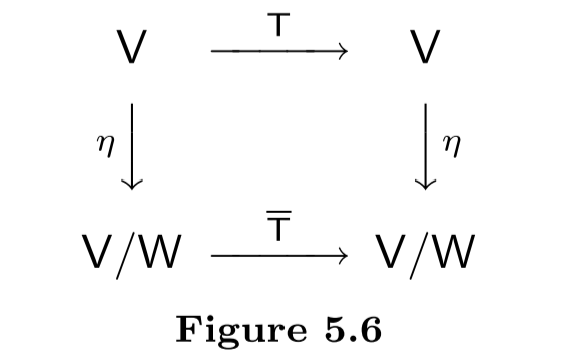
\includegraphics[width=8cm]{images/figure-5-6.png}

\end{exercise}

\begin{proof}
\end{proof}

\begin{exercise} \label{exercise 5.4.28}
Let \(f(t), g(t)\), and \(h(t)\) be the \CPOLY{} of \(\T, \T_W\), and \(\Tover\), respectively.
Prove that \(f(t) = g(t)h(t)\).
Hint: Extend an ordered basis \(\gamma = \{ v_1, v_2, ..., v_k \}\) for \(\W\) to an ordered basis \(\beta = \{ v_1, v_2, ..., v_k, v_{k + 1}, ..., v_n \}\) for \(\V\).
Then show that the \emph{collection of cosets} \(\alpha = \{ v_{k + 1} + \W, v_{k + 2} + \W, ..., v_n + \W \}\) is an ordered basis for \(\V/\W\), and prove that
\[
    [\T]_{\beta} = \begin{pmatrix}
        B_1 & B_2 \\ O B_3
    \end{pmatrix}.
\]
where \(B_1 = [\T_W]_{\gamma}\) and \(B_3 = [\Tover]_{\alpha}\).
\end{exercise}

\begin{proof}
這邊 \(B_1\) equal 的東西感覺有打錯。
\end{proof}

\begin{exercise} \label{exercise 5.4.29}
Use the hint in \EXEC{5.4.28} to prove that if \(\T\) is diagonalizable, then so is \(\Tover\).
\end{exercise}

\begin{proof}
\end{proof}

\begin{exercise} \label{exercise 5.4.30}
Prove that if both \(\T_W\) and \(\Tover\) are diagonalizable and \emph{have no common} eigenvalues, then \(\T\) is diagonalizable.
\end{exercise}

\begin{proof}
\end{proof}

The results of \THM{5.21} and \EXEC{5.4.28} are useful in devising \emph{methods for computing \CPOLY{}s} \textbf{without the use of determinants}.
This is illustrated in the next exercise.

\begin{exercise} \label{exercise 5.4.31}
Let \(A = \begin{pmatrix} 1 & 1 & -3 \\ 2 & 3 & 4 \\ 1 & 2 & 1 \end{pmatrix}\), let \(\T = \LMTRAN_A\), and let \(\W\) the cyclic subspace of \(\SET{R}^3\) generated by \(e_1\).

\begin{enumerate}
\item Use \THM{5.21} to compute the \CPOLY{} of \(\T_W\).
\item Show that \(\{ e_2 + \W \}\) is a basis for \(\SET{R}^3/\W\), and use this fact to compute the \CPOLY{} of \(\T\).
\item Use the results of (a) and (b) to find the \CPOLY{} of \(A\).
\end{enumerate}
\end{exercise}

\begin{proof}
\end{proof}

Exercises 32 through 39 are concerned with direct sums.

\begin{exercise} \label{exercise 5.4.32}
Let \(\T\) be a linear operator on a vector space \(\V\), and let \(W_1, W_2 , ..., W_k\) be \(\T\)-invariant subspaces of \(\V\).
Prove that \(W_1 + W_2 + ... + W_k\) is also a \(\T\)-invariant subspace of \(\V\).
\end{exercise}

\begin{proof}
\end{proof}

\begin{exercise} \label{exercise 5.4.33}
Give a \emph{direct proof} of \THM{5.24} for the case \(k = 2\).
(This result is used in the proof of \THM{5.23}.)
\end{exercise}

\begin{proof}
\end{proof}

\begin{exercise} \label{exercise 5.4.34}
Prove \THM{5.24}.
\emph{Hint}: Begin with \EXEC{5.4.33} and extend it using mathematical induction on \(k\), the number of subspaces.
\end{exercise}

\begin{proof}
\end{proof}

\begin{exercise} \label{exercise 5.4.35}
Let \(\T\) be a linear operator on a finite-dimensional vector space \(\V\).
Prove that \(\T\) is diagonalizable if and only if \(\V\) is the direct sum of \emph{one-dimensional} \(\T\)-invariant subspaces.
\end{exercise}

\begin{proof}
\end{proof}

\begin{exercise} \label{exercise 5.4.36}
Let \(\T\) be a linear operator on a finite-dimensional vector space \(\V\), and let \(W_1, W_2, ..., W_k\) be \(\T\)-invariant subspaces of \(\V\) such that \(v = W_1 \oplus W_2 \oplus ... \oplus W_k\).
Prove that
\[
    \det(\T) = \det(\T_{W_1}) \cdot \det(\T_{W_2}) \cdot \det(\T_{W_k}).
\]
\end{exercise}

\begin{proof}
\end{proof}

\begin{exercise} \label{exercise 5.4.37}
Let \(\T\) be a linear operator on a finite-dimensional vector space \(\V\), and let \(W_1, W_2, ..., W_k\) be \(\T\)-invariant subspaces of \(\V\) such that \(\V = W_1 \oplus W_2 \oplus ... \oplus W_k\).
Prove that \(\T\) is diagonalizable if and only if \(\T_W\), is diagonalizable for all \(i\).
\end{exercise}

\begin{proof}
\end{proof}

\begin{exercise} \label{exercise 5.4.38}
Let \(\mathcal{C}\) be an arbitrary collection of \emph{diagonalizable} linear operators on a finite-dimensional vector space \(\V\).
Prove that there is an ordered basis \(\beta\) such that \([\T]_{\beta}\) is a diagonal matrix for all \(\T \in \mathcal{C}\), if and only if, the operators of \(\mathcal{C}\) commute under composition.
(This is an extension of \EXEC{5.4.25}.)
Hints for the case that the operator commute:
The result is trivial if each operator has only one eigenvalue.
Otherwise, establish the general result by mathematical induction on \(\dim(\V)\), using the fact that \(\V\) is the direct sum of the eigenspaces of some operator in \(\mathcal{C}\) that has more than one eigenvalue.
\end{exercise}

\begin{proof}
\end{proof}

\begin{exercise} \label{exercise 5.4.39}
Let \(B_1, B_2, ..., B_k\) be square matrices with entries in the same field, and let \(A = B_1 \oplus B_2 \oplus ... \oplus B_k\).
Prove that the \CPOLY{} of \(A\) is the product of the \CPOLY{} of the \(B_i\)'s.
\end{exercise}

\begin{proof}
\end{proof}

\begin{exercise} \label{exercise 5.4.40}
Let
\[
    A = \begin{pmatrix}
        1 & 2 & ... & n \\
        n + 1 & n + 2  & ... & 2n \\
        \vdots & \vdots & & \vdots \\
        n^2 - n + 1 & n^2 - n + 2 & ... & n^2
    \end{pmatrix}.
\]
Find the \CPOLY{} of \(A\).
\emph{Hint}: First prove that \(A\) has rank \(21\) and that \(\spann(\{ (1, 1, ... , 1), (1, 2, ..., n) \})\) is \(\LMTRAN_A\)-invariant.
\end{exercise}

\begin{proof}
\end{proof}

\begin{exercise} \label{exercise 5.4.41}
Let \(A \in M_{n \X n}(\SET{R})\) be the matrix defined by \(A_{ij} = 1\) for all \(i\) and \(j\).
Find the \CPOLY{} of \(A\).
\end{exercise}

\begin{proof}
\end{proof}